%**************************************%
%*    Generated from PreTeXt source   *%
%*    on 2018-05-02T16:55:54-06:00    *%
%*                                    *%
%*   http://mathbook.pugetsound.edu   *%
%*                                    *%
%**************************************%
\documentclass[10pt,]{book}
%% Custom Preamble Entries, early (use latex.preamble.early)
%% Default LaTeX packages
%%   1.  always employed (or nearly so) for some purpose, or
%%   2.  a stylewriter may assume their presence
\usepackage{geometry}
%% Some aspects of the preamble are conditional,
%% the LaTeX engine is one such determinant
\usepackage{ifthen}
\usepackage{ifxetex,ifluatex}
%% Raster graphics inclusion
\usepackage{graphicx}
%% Colored boxes, and much more, though mostly styling
%% skins library provides "enhanced" skin, employing tikzpicture
%% boxes may be configured as "breakable" or "unbreakable"
%% "raster" controls grids of boxes, aka side-by-side
\usepackage{tcolorbox}
\tcbuselibrary{skins}
\tcbuselibrary{breakable}
\tcbuselibrary{raster}
%% xparse allows the construction of more robust commands,
%% this is a necessity for isolating styling and behavior
%% The tcolorbox library of the same name loads the base library
\tcbuselibrary{xparse}
%% Hyperref should be here, but likes to be loaded late
%%
%% Inline math delimiters, \(, \), need to be robust
%% 2016-01-31:  latexrelease.sty  supersedes  fixltx2e.sty
%% If  latexrelease.sty  exists, bugfix is in kernel
%% If not, bugfix is in  fixltx2e.sty
%% See:  https://tug.org/TUGboat/tb36-3/tb114ltnews22.pdf
%% and read "Fewer fragile commands" in distribution's  latexchanges.pdf
\IfFileExists{latexrelease.sty}{}{\usepackage{fixltx2e}}
%% Text height identically 9 inches, text width varies on point size
%% See Bringhurst 2.1.1 on measure for recommendations
%% 75 characters per line (count spaces, punctuation) is target
%% which is the upper limit of Bringhurst's recommendations
\geometry{letterpaper,total={340pt,9.0in}}
%% Custom Page Layout Adjustments (use latex.geometry)
\geometry{papersize={6in,9in}, hmargin={0.85in, 0.5in}, height=7.75in, top=0.75in, twoside, ignoreheadfoot}
%% This LaTeX file may be compiled with pdflatex, xelatex, or lualatex
%% The following provides engine-specific capabilities
%% Generally, xelatex and lualatex will do better languages other than US English
%% You can pick from the conditional if you will only ever use one engine
\ifthenelse{\boolean{xetex} \or \boolean{luatex}}{%
%% begin: xelatex and lualatex-specific configuration
%% fontspec package will make Latin Modern (lmodern) the default font
\ifxetex\usepackage{xltxtra}\fi
\usepackage{fontspec}
%% realscripts is the only part of xltxtra relevant to lualatex 
\ifluatex\usepackage{realscripts}\fi
%% 
%% Extensive support for other languages
\usepackage{polyglossia}
%% Main document language is US English
\setdefaultlanguage{english}
%% Spanish
\setotherlanguage{spanish}
%% Vietnamese
\setotherlanguage{vietnamese}
%% end: xelatex and lualatex-specific configuration
}{%
%% begin: pdflatex-specific configuration
%% translate common Unicode to their LaTeX equivalents
%% Also, fontenc with T1 makes CM-Super the default font
%% (\input{ix-utf8enc.dfu} from the "inputenx" package is possible addition (broken?)
\usepackage[T1]{fontenc}
\usepackage[utf8]{inputenc}
%% end: pdflatex-specific configuration
}
%% Monospace font: Inconsolata (zi4)
%% Sponsored by TUG: http://levien.com/type/myfonts/inconsolata.html
%% See package documentation for excellent instructions
%% One caveat, seem to need full file name to locate OTF files
%% Loads the "upquote" package as needed, so we don't have to
%% Upright quotes might come from the  textcomp  package, which we also use
%% We employ the shapely \ell to match Google Font version
%% pdflatex: "varqu" option produces best upright quotes
%% xelatex,lualatex: add StylisticSet 1 for shapely \ell
%% xelatex,lualatex: add StylisticSet 2 for plain zero
%% xelatex,lualatex: we add StylisticSet 3 for upright quotes
%% 
\ifthenelse{\boolean{xetex} \or \boolean{luatex}}{%
%% begin: xelatex and lualatex-specific monospace font
\usepackage{zi4}
\setmonofont[BoldFont=Inconsolatazi4-Bold.otf,StylisticSet={1,3}]{Inconsolatazi4-Regular.otf}
%% end: xelatex and lualatex-specific monospace font
}{%
%% begin: pdflatex-specific monospace font
%% "varqu" option provides textcomp \textquotedbl glyph
%% "varl"  option provides shapely "ell"
\usepackage[varqu,varl]{zi4}
%% end: pdflatex-specific monospace font
}
%% \mono macro for content of "c" element only
\newcommand{\mono}[1]{\texttt{#1}}
%% Symbols, align environment, bracket-matrix
\usepackage{amsmath}
\usepackage{amssymb}
%% allow page breaks within display mathematics anywhere
%% level 4 is maximally permissive
%% this is exactly the opposite of AMSmath package philosophy
%% there are per-display, and per-equation options to control this
%% split, aligned, gathered, and alignedat are not affected
\allowdisplaybreaks[4]
%% allow more columns to a matrix
%% can make this even bigger by overriding with  latex.preamble.late  processing option
\setcounter{MaxMatrixCols}{30}
%%
%% Color support, xcolor package
%% Always loaded, for: add/delete text, author tools
\PassOptionsToPackage{usenames,dvipsnames,svgnames,table}{xcolor}
\usepackage{xcolor}
%%
%% Semantic Macros
%% To preserve meaning in a LaTeX file
%% Only defined here if required in this document
%% Used for inline definitions of terms
\newcommand{\terminology}[1]{\textbf{#1}}
%% Subdivision Numbering, Chapters, Sections, Subsections, etc
%% Subdivision numbers may be turned off at some level ("depth")
%% A section *always* has depth 1, contrary to us counting from the document root
%% The latex default is 3.  If a larger number is present here, then
%% removing this command may make some cross-references ambiguous
%% The precursor variable $numbering-maxlevel is checked for consistency in the common XSL file
\setcounter{secnumdepth}{1}
%% Environments with amsthm package
%% Theorem-like environments in "plain" style, with or without proof
\usepackage{amsthm}
\theoremstyle{plain}
%% Numbering for Theorems, Conjectures, Examples, Figures, etc
%% Controlled by  numbering.theorems.level  processing parameter
%% Always need a theorem environment to set base numbering scheme
%% even if document has no theorems (but has other environments)
\newtheorem{theorem}{Theorem}[section]
%% Only variants actually used in document appear here
%% Style is like a theorem, and for statements without proofs
%% Numbering: all theorem-like numbered consecutively
%% i.e. Corollary 4.3 follows Theorem 4.2
%% Example-like environments, normal text
%% Numbering is in sync with theorems, etc
\theoremstyle{definition}
\newtheorem{example}[theorem]{Example}
%% Numbering for Projects (independent of others)
%% Controlled by  numbering.projects.level  processing parameter
%% Always need a project environment to set base numbering scheme
%% even if document has no projectss (but has other blocks)
\newtheorem{project}{Project}%% Project-like environments, normal text
\theoremstyle{definition}
\newtheorem{investigation}[project]{Investigate!}
%% begin: assemblage
%% minimally structured content, high visibility presentation
%% One optional argument (title) with default value blank
%% 3mm space below dropped title is increase over 2mm default
\newtcolorbox{assemblage}[1][]
  {breakable, skin=enhanced, arc=2ex, colback=blue!5, colframe=blue!75!black,
   colbacktitle=blue!20, coltitle=black, boxed title style={sharp corners, frame hidden},
   fonttitle=\bfseries, attach boxed title to top left={xshift=4mm,yshift=-3mm}, top=3mm, title={#1}}
%% end: assemblage
%% Localize LaTeX supplied names (possibly none)
\renewcommand*{\proofname}{Proof}
\renewcommand*{\chaptername}{Chapter}
%% Equation Numbering
%% Controlled by  numbering.equations.level  processing parameter
\numberwithin{equation}{chapter}
%% For improved tables
\usepackage{array}
%% Some extra height on each row is desirable, especially with horizontal rules
%% Increment determined experimentally
\setlength{\extrarowheight}{0.2ex}
%% Define variable thickness horizontal rules, full and partial
%% Thicknesses are 0.03, 0.05, 0.08 in the  booktabs  package
\makeatletter
\newcommand{\hrulethin}  {\noalign{\hrule height 0.04em}}
\newcommand{\hrulemedium}{\noalign{\hrule height 0.07em}}
\newcommand{\hrulethick} {\noalign{\hrule height 0.11em}}
%% We preserve a copy of the \setlength package before other
%% packages (extpfeil) get a chance to load packages that redefine it
\let\oldsetlength\setlength
\newlength{\Oldarrayrulewidth}
\newcommand{\crulethin}[1]%
{\noalign{\global\oldsetlength{\Oldarrayrulewidth}{\arrayrulewidth}}%
\noalign{\global\oldsetlength{\arrayrulewidth}{0.04em}}\cline{#1}%
\noalign{\global\oldsetlength{\arrayrulewidth}{\Oldarrayrulewidth}}}%
\newcommand{\crulemedium}[1]%
{\noalign{\global\oldsetlength{\Oldarrayrulewidth}{\arrayrulewidth}}%
\noalign{\global\oldsetlength{\arrayrulewidth}{0.07em}}\cline{#1}%
\noalign{\global\oldsetlength{\arrayrulewidth}{\Oldarrayrulewidth}}}
\newcommand{\crulethick}[1]%
{\noalign{\global\oldsetlength{\Oldarrayrulewidth}{\arrayrulewidth}}%
\noalign{\global\oldsetlength{\arrayrulewidth}{0.11em}}\cline{#1}%
\noalign{\global\oldsetlength{\arrayrulewidth}{\Oldarrayrulewidth}}}
%% Single letter column specifiers defined via array package
\newcolumntype{A}{!{\vrule width 0.04em}}
\newcolumntype{B}{!{\vrule width 0.07em}}
\newcolumntype{C}{!{\vrule width 0.11em}}
\makeatother
%% Footnote Numbering
%% We reset the footnote counter, as given by numbering.footnotes.level
\makeatletter\@addtoreset{footnote}{chapter}\makeatother
%% More flexible list management, esp. for references and exercises
%% But also for specifying labels (i.e. custom order) on nested lists
\usepackage{enumitem}
%% Lists of exercises in their own section, maximum depth 4
\newlist{exerciselist}{description}{4}
\setlist[exerciselist]{leftmargin=0pt,itemsep=1.0ex,topsep=1.0ex,partopsep=0pt,parsep=0pt}
%% Package for tables spanning several pages
\usepackage{longtable}
%% hyperref driver does not need to be specified, it will be detected
\usepackage{hyperref}
%% configure hyperref's  \url  to match listings' inline verbatim
\renewcommand\UrlFont{\small\ttfamily}
%% Hyperlinking active in PDFs, all links solid and blue
\hypersetup{colorlinks=true,linkcolor=blue,citecolor=blue,filecolor=blue,urlcolor=blue}
\hypersetup{pdftitle={Discrete Mathematics}}
%% If you manually remove hyperref, leave in this next command
\providecommand\phantomsection{}
%% Graphics Preamble Entries
\usepackage{tikz, pgfplots}

\usetikzlibrary{positioning,matrix,arrows}

\usetikzlibrary{shapes,decorations,shadows,fadings,patterns}
\usetikzlibrary{decorations.markings}

\usepackage{skak} %for chessboards etc.


\def\circleA{(-.5,0) circle (1)}
\def\circleAlabel{(-1.5,.6) node[above]{$A$}}
\def\circleB{(.5,0) circle (1)}
\def\circleBlabel{(1.5,.6) node[above]{$B$}}
\def\circleC{(0,-1) circle (1)}
\def\circleClabel{(.5,-2) node[right]{$C$}}
\def\twosetbox{(-2,-1.4) rectangle (2,1.4)}
\def\threesetbox{(-2.5,-2.4) rectangle (2.5,1.4)}
\newcommand{\hexbox}[3]{
  \def\x{-cos{30}*\r*#1+cos{30}*#2*\r*2}
  \def\y{-\r*#1-sin{30}*\r*#1}
  \draw (\x,\y) +(90:\r) -- +(30:\r) -- +(-30:\r) -- +(-90:\r) -- +(-150:\r) -- +(150:\r) -- cycle;
  \draw (\x,\y) node{#3};
}

\tikzset{->-/.style={decoration={
  markings,
  mark=at position .5 with {\arrow{>}}},postaction={decorate}}}


%% Imported from https://upload.wikimedia.org/wikipedia/commons/3/32/Blank_US_Map.svg
%% Translated to TikZ using Inkscape 0.48
%% From https://gist.github.com/bordaigorl/fce575813ff943f47505

\tikzset{USA map/.cd,
state/.style={fill, draw=white, ultra thick},
HI/.style={}, AK/.style={}, FL/.style={}, NH/.style={}, MI/.style={}, MI/.style={}, SP/.style={}, VT/.style={}, ME/.style={}, RI/.style={}, NY/.style={}, PA/.style={}, NJ/.style={}, DE/.style={}, MD/.style={}, VA/.style={}, WV/.style={}, OH/.style={}, IN/.style={}, IL/.style={}, CT/.style={}, WI/.style={}, NC/.style={}, DC/.style={}, MA/.style={}, TN/.style={}, AR/.style={}, MO/.style={}, GA/.style={}, SC/.style={}, KY/.style={}, AL/.style={}, LA/.style={}, MS/.style={}, IA/.style={}, MN/.style={}, OK/.style={}, TX/.style={}, NM/.style={}, KS/.style={}, NE/.style={}, SD/.style={}, ND/.style={}, WY/.style={}, MT/.style={}, CO/.style={}, ID/.style={}, UT/.style={}, AZ/.style={}, NV/.style={}, OR/.style={}, WA/.style={}, CA/.style={}}

\tikzset{
every state/.style={USA map/state/.style={#1}},
HI/.style={USA map/HI/.style={#1}}, AK/.style={USA map/AK/.style={#1}}, FL/.style={USA map/FL/.style={#1}}, NH/.style={USA map/NH/.style={#1}}, MI/.style={USA map/MI/.style={#1}}, SP/.style={USA map/SP/.style={#1}}, VT/.style={USA map/VT/.style={#1}}, ME/.style={USA map/ME/.style={#1}}, RI/.style={USA map/RI/.style={#1}}, NY/.style={USA map/NY/.style={#1}}, PA/.style={USA map/PA/.style={#1}}, NJ/.style={USA map/NJ/.style={#1}}, DE/.style={USA map/DE/.style={#1}}, MD/.style={USA map/MD/.style={#1}}, VA/.style={USA map/VA/.style={#1}}, WV/.style={USA map/WV/.style={#1}}, OH/.style={USA map/OH/.style={#1}}, IN/.style={USA map/IN/.style={#1}}, IL/.style={USA map/IL/.style={#1}}, CT/.style={USA map/CT/.style={#1}}, WI/.style={USA map/WI/.style={#1}}, NC/.style={USA map/NC/.style={#1}}, DC/.style={USA map/DC/.style={#1}}, MA/.style={USA map/MA/.style={#1}}, TN/.style={USA map/TN/.style={#1}}, AR/.style={USA map/AR/.style={#1}}, MO/.style={USA map/MO/.style={#1}}, GA/.style={USA map/GA/.style={#1}}, SC/.style={USA map/SC/.style={#1}}, KY/.style={USA map/KY/.style={#1}}, AL/.style={USA map/AL/.style={#1}}, LA/.style={USA map/LA/.style={#1}}, MS/.style={USA map/MS/.style={#1}}, IA/.style={USA map/IA/.style={#1}}, MN/.style={USA map/MN/.style={#1}}, OK/.style={USA map/OK/.style={#1}}, TX/.style={USA map/TX/.style={#1}}, NM/.style={USA map/NM/.style={#1}}, KS/.style={USA map/KS/.style={#1}}, NE/.style={USA map/NE/.style={#1}}, SD/.style={USA map/SD/.style={#1}}, ND/.style={USA map/ND/.style={#1}}, WY/.style={USA map/WY/.style={#1}}, MT/.style={USA map/MT/.style={#1}}, CO/.style={USA map/CO/.style={#1}}, ID/.style={USA map/ID/.style={#1}}, UT/.style={USA map/UT/.style={#1}}, AZ/.style={USA map/AZ/.style={#1}}, NV/.style={USA map/NV/.style={#1}}, OR/.style={USA map/OR/.style={#1}}, WA/.style={USA map/WA/.style={#1}}, CA/.style={USA map/CA/.style={#1}}
}

\newcommand{\USA}[1][]{
    \begin{scope}[y=0.80pt,x=0.80pt,yscale=-1, inner sep=0pt, outer sep=0pt,
    #1
    ]

    % HI
    \path[USA map/state, USA map/HI, local bounding box=HI] (233.0875,519.3095) -- (235.0274,515.7529) -- (237.2907,515.4296) --
      (237.6140,516.2379) -- (235.5124,519.3095) -- (233.0875,519.3095) --
      cycle(243.2722,515.5913) -- (249.4153,518.1778) -- (251.5169,517.8545) --
      (253.1335,513.9747) -- (252.4869,510.5798) -- (248.2837,510.0948) --
      (244.2421,511.8731) -- (243.2722,515.5913) -- cycle(273.9878,525.6143) --
      (277.7060,531.1107) -- (280.1309,530.7874) -- (281.2625,530.3024) --
      (282.7175,531.5957) -- (286.4357,531.4341) -- (287.4057,529.9791) --
      (284.4958,528.2009) -- (282.5558,524.4826) -- (280.4542,520.9261) --
      (274.6344,523.8360) -- (273.9878,525.6143) -- cycle(294.1954,534.5056) --
      (295.4887,532.5657) -- (300.1769,533.5357) -- (300.8236,533.0507) --
      (306.9667,533.6973) -- (306.6434,534.9906) -- (304.0568,536.4456) --
      (299.6919,536.1222) -- (294.1954,534.5056) -- cycle(299.5303,539.6788) --
      (301.4702,543.5587) -- (304.5418,542.4270) -- (304.8651,540.8104) --
      (303.2485,538.7088) -- (299.5303,538.3855) -- (299.5303,539.6788) --
      cycle(306.4817,538.5472) -- (308.7450,535.6373) -- (313.4331,538.0622) --
      (317.7980,539.1938) -- (322.1628,541.9421) -- (322.1628,543.8820) --
      (318.6063,545.6603) -- (313.7565,546.6302) -- (311.3315,545.1753) --
      (306.4817,538.5472) -- cycle(323.1328,554.0666) -- (324.7494,552.7734) --
      (328.1443,554.3900) -- (335.7424,557.9465) -- (339.1373,560.0481) --
      (340.7539,562.4730) -- (342.6938,566.8379) -- (346.7353,569.4245) --
      (346.4120,570.7178) -- (342.5321,573.9510) -- (338.3290,575.4059) --
      (336.8740,574.7593) -- (333.8024,576.5375) -- (331.3775,579.7708) --
      (329.1143,582.6807) -- (327.3360,582.5190) -- (323.7794,579.9324) --
      (323.4561,575.4059) -- (324.1028,572.9810) -- (322.4862,567.3229) --
      (320.3846,565.5446) -- (320.2229,562.9580) -- (322.4862,561.9880) --
      (324.5878,558.9165) -- (325.0727,557.9465) -- (323.4561,556.1682) --
      (323.1328,554.0666) -- cycle;

    % AK
    \path[USA map/state, USA map/AK, local bounding box=AK] (158.0767,453.6750) -- (157.7534,539.0322) -- (159.3700,540.0021) --
      (162.4416,540.1638) -- (163.8965,539.0322) -- (166.4831,539.0322) --
      (166.6447,541.9420) -- (173.5962,548.7318) -- (174.0812,551.3184) --
      (177.4760,549.3785) -- (178.1227,549.2168) -- (178.4460,546.1452) --
      (179.9010,544.5286) -- (181.0326,544.3670) -- (182.9725,542.9120) --
      (186.0441,545.0136) -- (186.6907,547.9235) -- (188.6307,549.0551) --
      (189.7623,551.4801) -- (193.6422,553.2583) -- (197.0371,559.2398) --
      (199.7853,563.1197) -- (202.0486,565.8679) -- (203.5035,569.5861) --
      (208.5150,571.3644) -- (213.6882,573.4660) -- (214.6581,577.8308) --
      (215.1431,580.9024) -- (214.1732,584.2973) -- (212.3949,586.5605) --
      (210.7783,585.7522) -- (209.3233,582.6807) -- (206.5751,581.2257) --
      (204.7968,580.0941) -- (203.9885,580.9024) -- (205.4434,583.6507) --
      (205.6051,587.3689) -- (204.4735,587.8538) -- (202.5335,585.9139) --
      (200.4320,584.6206) -- (200.9169,586.2372) -- (202.2102,588.0155) --
      (201.4019,588.8238) .. controls (201.4019,588.8238) and (200.5936,588.5005) ..
      (200.1086,587.8538) .. controls (199.6236,587.2072) and (198.0070,584.4590) ..
      (198.0070,584.4590) -- (197.0371,582.1957) .. controls (197.0371,582.1957) and
      (196.7137,583.4890) .. (196.0671,583.1657) .. controls (195.4204,582.8423) and
      (194.7738,581.7107) .. (194.7738,581.7107) -- (196.5521,579.7708) --
      (195.0971,578.3158) -- (195.0971,573.3043) -- (194.2888,573.3043) --
      (193.4805,576.6992) -- (192.3489,577.1842) -- (191.3789,573.4660) --
      (190.7323,569.7478) -- (189.9240,569.2628) -- (190.2473,574.9209) --
      (190.2473,576.0526) -- (188.7923,574.7593) -- (185.2358,568.7778) --
      (183.1342,568.2928) -- (182.4876,564.5746) -- (180.8709,561.6647) --
      (179.2543,560.5331) -- (179.2543,558.2698) -- (181.3559,556.9765) --
      (180.8709,556.6532) -- (178.2844,557.2999) -- (174.8895,554.8750) --
      (172.3029,551.9650) -- (167.4531,549.3785) -- (163.4115,546.7919) --
      (164.7048,543.5587) -- (164.7048,541.9421) -- (162.9265,543.5587) --
      (160.0166,544.6903) -- (156.2984,543.5587) -- (150.6403,541.1338) --
      (145.1438,541.1338) -- (144.4972,541.6187) -- (138.0307,537.7389) --
      (135.9291,537.4155) -- (133.1809,531.5957) -- (129.6243,531.9191) --
      (126.0678,533.3740) -- (126.5528,537.9005) -- (127.6844,534.9906) --
      (128.6544,535.3139) -- (127.1994,539.6788) -- (130.4326,536.9306) --
      (131.0793,538.5472) -- (127.1994,542.9120) -- (125.9061,542.5887) --
      (125.4211,540.6488) -- (124.1279,539.8405) -- (122.8346,540.9721) --
      (120.0863,539.1938) -- (117.0148,541.2954) -- (115.2365,543.3970) --
      (111.8416,545.4986) -- (107.1534,545.3369) -- (106.6684,543.2353) --
      (110.3866,542.5887) -- (110.3866,541.2954) -- (108.1234,540.6488) --
      (109.0934,538.2238) -- (111.3566,534.3440) -- (111.3566,532.5657) --
      (111.5183,531.7574) -- (115.8831,529.4941) -- (116.8531,530.7874) --
      (119.6013,530.7874) -- (118.3081,528.2009) -- (114.5898,527.8775) --
      (109.5783,530.6258) -- (107.1534,534.0206) -- (105.3752,536.6072) --
      (104.2435,538.8705) -- (100.0403,540.3254) -- (96.9688,542.9120) --
      (96.6454,544.5286) -- (98.9087,545.4986) -- (99.7170,547.6002) --
      (96.9688,550.8334) -- (90.5023,555.0366) -- (82.7426,559.2398) --
      (80.6410,560.3714) -- (75.3062,561.5031) -- (69.9713,563.7663) --
      (71.7496,565.0596) -- (70.2947,566.5146) -- (69.8097,567.6462) --
      (67.0614,566.6762) -- (63.8282,566.8379) -- (63.0199,569.1011) --
      (62.0499,569.1011) -- (62.3733,566.6762) -- (58.8167,567.9695) --
      (55.9068,568.9395) -- (52.5119,567.6462) -- (49.6020,569.5861) --
      (46.3688,569.5861) -- (44.2672,570.8794) -- (42.6506,571.6877) --
      (40.5490,571.3644) -- (37.9624,570.2328) -- (35.6992,570.8794) --
      (34.7292,571.8494) -- (33.1126,570.7178) -- (33.1126,568.7778) --
      (36.1841,567.4845) -- (42.4889,568.1312) -- (46.8538,566.5146) --
      (48.9554,564.4130) -- (51.8653,563.7663) -- (53.6436,562.9580) --
      (56.3918,563.1197) -- (58.0084,564.4130) -- (58.9784,564.0896) --
      (61.2416,561.3414) -- (64.3132,560.3714) -- (67.7081,559.7248) --
      (69.0014,559.4015) -- (69.6480,559.8864) -- (70.4563,559.8864) --
      (71.7496,556.1682) -- (75.7911,554.7133) -- (77.7311,550.9951) --
      (79.9943,546.4686) -- (81.6110,545.0136) -- (81.9343,542.4270) --
      (80.3177,543.7203) -- (76.9228,544.3670) -- (76.2761,541.9421) --
      (74.9828,541.6187) -- (74.0129,542.5887) -- (73.8512,545.4986) --
      (72.3963,545.3369) -- (70.9413,539.5171) -- (69.6480,540.8104) --
      (68.5164,540.3254) -- (68.1931,538.3855) -- (64.1515,538.5472) --
      (62.0499,539.6788) -- (59.4634,539.3555) -- (60.9183,537.9005) --
      (61.4033,535.3139) -- (60.7566,533.3740) -- (62.2116,532.4040) --
      (63.5049,532.2424) -- (62.8582,530.4641) -- (62.8582,526.0993) --
      (61.8883,525.1293) -- (61.0800,526.5842) -- (54.9368,526.5842) --
      (53.4819,525.2909) -- (52.8352,521.4111) -- (50.7337,517.8545) --
      (50.7337,516.8846) -- (52.8352,516.0763) -- (52.9969,513.9747) --
      (54.1285,512.8430) -- (53.3202,512.3581) -- (52.0269,512.8430) --
      (50.8953,510.0948) -- (51.8653,505.0833) -- (56.3918,501.8501) --
      (58.9784,500.2335) -- (60.9183,496.5153) -- (63.6666,495.2220) --
      (66.2531,496.3536) -- (66.5765,498.7785) -- (69.0014,498.4552) --
      (72.2346,496.0303) -- (73.8512,496.6769) -- (74.8212,497.3236) --
      (76.4378,497.3236) -- (78.7010,496.0303) -- (79.5094,491.6654) .. controls
      (79.5094,491.6654) and (79.8327,488.7555) .. (80.4793,488.2705) .. controls
      (81.1260,487.7855) and (81.4493,487.3006) .. (81.4493,487.3006) --
      (80.3177,485.3606) -- (77.7311,486.1689) -- (74.4978,486.9772) --
      (72.5579,486.4923) -- (69.0014,484.7140) -- (63.9899,484.5523) --
      (60.4333,480.8341) -- (60.9183,476.9542) -- (61.5650,474.5293) --
      (59.4634,472.7511) -- (57.5234,469.0328) -- (58.0084,468.2245) --
      (64.7982,467.7396) -- (66.8998,467.7396) -- (67.8697,468.7095) --
      (68.5164,468.7095) -- (68.3547,467.0929) -- (72.2346,466.4463) --
      (74.8212,466.7696) -- (76.2761,467.9012) -- (74.8212,470.0028) --
      (74.3362,471.4578) -- (77.0844,473.0744) -- (82.0959,474.8526) --
      (83.8742,473.8827) -- (81.6110,469.5178) -- (80.6410,466.2846) --
      (81.6110,465.4763) -- (78.2161,463.5364) -- (77.7311,462.4047) --
      (78.2161,460.7881) -- (77.4078,456.9083) -- (74.4978,452.2201) --
      (72.0729,448.0169) -- (74.9828,446.0769) -- (78.2161,446.0769) --
      (79.9943,446.7236) -- (84.1975,446.5619) -- (87.9157,443.0054) --
      (89.0474,439.9338) -- (92.7656,437.5089) -- (94.3822,438.4789) --
      (97.1304,437.8322) -- (100.8486,435.7306) -- (101.9803,435.5690) --
      (102.9502,436.3773) -- (107.4767,436.2156) -- (110.2250,433.1441) --
      (111.3566,433.1441) -- (114.9132,435.5690) -- (116.8531,437.6706) --
      (116.3681,438.8022) -- (117.0148,439.9338) -- (118.6314,438.3172) --
      (122.5112,438.6405) -- (122.8346,442.3587) -- (124.7745,443.8137) --
      (131.8876,444.4603) -- (138.1924,448.6635) -- (139.6473,447.6936) --
      (144.8205,450.2801) -- (146.9221,449.6335) -- (148.8620,448.8252) --
      (153.7119,450.7651) -- (158.0767,453.6750) -- cycle(42.9739,482.6124) --
      (45.0755,487.9472) -- (44.9138,488.9172) -- (42.0039,488.5938) --
      (40.2257,484.5523) -- (38.4474,483.0974) -- (36.0225,483.0974) --
      (35.8608,480.5108) -- (37.6391,478.0859) -- (38.7707,480.5108) --
      (40.2257,481.9657) -- (42.9739,482.6124) -- cycle(40.3873,516.0763) --
      (44.1055,516.8846) -- (47.8237,517.8545) -- (48.6321,518.8245) --
      (47.0154,522.5427) -- (43.9439,522.3810) -- (40.5490,518.8245) --
      (40.3873,516.0763) -- cycle(19.6947,502.0117) -- (20.8263,504.5983) --
      (21.9580,506.2149) -- (20.8263,507.0232) -- (18.7247,503.9517) --
      (18.7247,502.0117) -- (19.6947,502.0117) -- cycle(5.9535,575.0826) --
      (9.3484,572.8193) -- (12.7433,571.8494) -- (15.3298,572.1727) --
      (15.8148,573.7893) -- (17.7548,574.2743) -- (19.6947,572.3344) --
      (19.3714,570.7178) -- (22.1196,570.0711) -- (25.0295,572.6577) --
      (23.8979,574.4360) -- (19.5330,575.5676) -- (16.7848,575.0826) --
      (13.0666,573.9510) -- (8.7017,575.4059) -- (7.0851,575.7292) --
      (5.9535,575.0826) -- cycle(54.9368,570.5561) -- (56.5535,572.4960) --
      (58.6550,570.8794) -- (57.2001,569.5861) -- (54.9368,570.5561) --
      cycle(57.8467,573.6276) -- (58.9784,571.3644) -- (61.0800,571.6877) --
      (60.2717,573.6276) -- (57.8467,573.6276) -- cycle(81.4493,571.6877) --
      (82.9042,573.4660) -- (83.8742,572.3344) -- (83.0659,570.3944) --
      (81.4493,571.6877) -- cycle(90.1790,559.2398) -- (91.3106,565.0596) --
      (94.2205,565.8679) -- (99.2320,562.9580) -- (103.5969,560.3714) --
      (101.9803,557.9465) -- (102.4652,555.5216) -- (100.3636,556.8149) --
      (97.4538,556.0066) -- (99.0704,554.8750) -- (101.0103,555.6833) --
      (104.8902,553.9050) -- (105.3751,552.4500) -- (102.9502,551.6417) --
      (103.7585,549.7018) -- (101.0103,551.6417) -- (96.3221,555.1983) --
      (91.4723,558.1082) -- (90.1790,559.2398) -- cycle(132.5342,539.3555) --
      (134.9592,537.9005) -- (133.9892,536.1222) -- (132.2109,537.0922) --
      (132.5342,539.3555) -- cycle;

    % FL
    \path[USA map/state, USA map/FL, local bounding box=FL] (759.8167,439.1428) -- (762.0824,446.4614) -- (765.8121,456.2037) --
      (771.1468,465.5800) -- (774.8650,471.8847) -- (779.7149,477.3812) --
      (783.7564,481.0994) -- (785.3730,484.0093) -- (784.2414,485.3025) --
      (783.4330,486.5958) -- (786.3429,494.0322) -- (789.2528,496.9421) --
      (791.8394,502.2769) -- (795.3959,508.0967) -- (799.9224,516.3413) --
      (801.2157,523.9394) -- (801.7007,535.9023) -- (802.3473,537.6805) --
      (802.0240,541.0754) -- (799.5991,542.3687) -- (799.9224,544.3086) --
      (799.2758,546.2485) -- (799.5991,548.6734) -- (800.0841,550.6134) --
      (797.3358,553.8466) -- (794.2643,555.3015) -- (790.3844,555.4632) --
      (788.9295,557.0798) -- (786.5046,558.0497) -- (785.2113,557.5648) --
      (784.0797,556.5948) -- (783.7564,553.6849) -- (782.9481,550.2900) --
      (779.5532,545.1169) -- (775.9967,542.8537) -- (772.1168,542.5303) --
      (771.3085,543.8236) -- (768.2370,539.4588) -- (767.5903,535.9023) --
      (765.0037,531.8608) -- (763.2255,530.7291) -- (761.6089,532.8307) --
      (759.8306,532.5074) -- (757.7290,527.4959) -- (754.8191,523.6161) --
      (751.9092,518.2813) -- (749.3227,515.2097) -- (745.7662,511.4915) --
      (747.8677,509.0666) -- (751.1009,503.5702) -- (750.9393,501.9536) --
      (746.4128,500.9836) -- (744.7962,501.6302) -- (745.1195,502.2769) --
      (747.7061,503.2468) -- (746.2511,507.7733) -- (745.4428,508.2583) --
      (743.6646,504.2168) -- (742.3713,499.3670) -- (742.0480,496.6188) --
      (743.5029,491.9306) -- (743.5029,482.3927) -- (740.4314,478.6745) --
      (739.1381,475.6029) -- (733.9649,474.3096) -- (732.0250,473.6630) --
      (730.4084,471.0764) -- (727.0135,469.4598) -- (725.8819,466.0649) --
      (723.1337,465.0950) -- (720.7088,461.3768) -- (716.5056,459.9219) --
      (713.5957,458.4669) -- (711.0092,458.4669) -- (706.9676,459.2752) --
      (706.8060,461.2151) -- (707.6143,462.1851) -- (707.1293,463.3167) --
      (704.0578,463.1551) -- (700.3396,466.7116) -- (696.7830,468.6515) --
      (692.9032,468.6515) -- (689.6700,469.9448) -- (689.3466,467.1966) --
      (687.7300,465.2566) -- (684.8202,464.1250) -- (683.2036,462.6701) --
      (675.1205,458.7902) -- (667.5225,457.0120) -- (663.1577,457.6586) --
      (657.1762,458.1436) -- (651.1948,460.2452) -- (647.7155,460.8581) --
      (647.4776,452.8084) -- (644.8910,450.8685) -- (643.1128,449.0902) --
      (643.4361,446.0186) -- (653.6207,444.7254) -- (679.1631,441.8155) --
      (685.9529,441.1688) -- (691.3889,441.4491) -- (693.9754,445.3290) --
      (695.4304,446.7839) -- (703.5285,447.2991) -- (714.3483,446.6525) --
      (735.8607,445.3592) -- (741.3064,444.6848) -- (746.4140,444.8893) --
      (746.8408,447.7992) -- (749.0738,448.6075) -- (749.3087,443.9775) --
      (747.7805,439.8046) -- (749.0889,438.3647) -- (754.6436,438.8195) --
      (759.8167,439.1428) -- cycle(772.3621,571.5479) -- (774.7870,570.9012) --
      (776.0803,570.6588) -- (777.5353,568.3147) -- (779.8793,566.6980) --
      (781.1726,567.1830) -- (782.8701,567.5064) -- (783.2742,568.5571) --
      (779.7985,569.7696) -- (775.5953,571.2246) -- (773.2512,572.4370) --
      (772.3621,571.5479) -- cycle(785.8608,566.5364) -- (787.0733,567.5872) --
      (789.8215,565.4856) -- (795.1563,561.2824) -- (798.8745,557.4025) --
      (801.3803,550.7744) -- (802.3502,549.0770) -- (802.5119,545.6821) --
      (801.7844,546.1671) -- (800.8145,548.9962) -- (799.3595,553.6035) --
      (796.1263,558.8575) -- (791.7614,563.0607) -- (788.3666,565.0006) --
      (785.8608,566.5364) -- cycle;

    % NH
    \path[USA map/state, USA map/NH, local bounding box=NH] (880.7990,142.4248) -- (881.6680,141.3483) -- (882.7582,138.0572) --
      (880.2152,137.1438) -- (879.7302,134.0722) -- (875.8503,132.9406) --
      (875.5270,130.1923) -- (868.2523,106.7515) -- (863.6508,92.2085) --
      (862.7538,92.2034) -- (862.1071,93.8200) -- (861.4605,93.3351) --
      (860.4905,92.3651) -- (859.0356,94.3050) -- (858.9871,99.3371) --
      (859.2987,105.0043) -- (861.2386,107.7525) -- (861.2386,111.7941) --
      (857.5204,116.8568) -- (854.9339,117.9885) -- (854.9339,119.1201) --
      (856.0655,120.8984) -- (856.0655,129.4664) -- (855.2572,138.6811) --
      (855.0955,143.5309) -- (856.0655,144.8242) -- (855.9038,149.3507) --
      (855.4188,151.1289) -- (856.3876,151.8382) -- (873.1753,147.4136) --
      (875.3502,146.8112) -- (877.1938,144.0378) -- (880.7990,142.4247) -- cycle;

    % % path57
    % \path[USA map/state, USA map/draw, local bounding box=draw[path57]=ca9a9a9,line width=1.600pt] (211.0000,493.0000) --
    %   (211.0000,548.0000) -- (247.0000,593.0000)(0.0000,425.0000) --
    %   (144.0000,425.0000) -- (211.0000,493.0000) -- (297.0000,493.0000) --
    %   (350.0000,547.0000) -- (350.0000,593.0000);

    \begin{scope}% MI
      % MI-
    \path[USA map/state, USA map/MI, local bounding box=MI] (697.8601,177.2369) -- (694.6269,168.9922)
        -- (692.3636,159.9392) -- (689.9387,156.7060) -- (687.3521,154.9277) --
        (685.7355,156.0594) -- (681.8557,157.8376) -- (679.9158,162.8491) --
        (677.1675,166.5673) -- (676.0359,167.2139) -- (674.5810,166.5673) .. controls
        (674.5810,166.5673) and (671.9944,165.1123) .. (672.1561,164.4657) .. controls
        (672.3177,163.8191) and (672.6410,159.4542) .. (672.6410,159.4542) --
        (676.0359,158.1609) -- (676.8442,154.7661) -- (677.4908,152.1795) --
        (679.9158,150.5629) -- (679.5924,140.5400) -- (677.9758,138.2767) --
        (676.6825,137.4684) -- (675.8742,135.3668) -- (676.6825,134.5585) --
        (678.2991,134.8818) -- (678.4608,133.2652) -- (676.0359,131.0020) --
        (674.7426,128.4154) -- (672.1561,128.4154) -- (667.6296,126.9605) --
        (662.1331,123.5656) -- (659.3849,123.5656) -- (658.7382,124.2123) --
        (657.7683,123.7273) -- (654.6967,121.4640) -- (651.7868,123.2423) --
        (648.8769,125.5055) -- (649.2003,129.0621) -- (650.1702,129.3854) --
        (652.2718,129.8704) -- (652.7568,130.6787) -- (650.1702,131.4870) --
        (647.5837,131.8103) -- (646.1287,133.5886) -- (645.8054,135.6901) --
        (646.1287,137.3067) -- (646.4520,142.8032) -- (642.8955,144.9048) --
        (642.2489,144.7431) -- (642.2489,140.5400) -- (643.5421,138.1151) --
        (644.1888,135.6901) -- (643.3805,134.8818) -- (641.4406,135.6901) --
        (640.4706,139.8933) -- (637.7224,141.0249) -- (635.9441,142.9649) --
        (635.7824,143.9348) -- (636.4291,144.7431) -- (635.7824,147.3297) --
        (633.5192,147.8147) -- (633.5192,148.9463) -- (634.3275,151.3712) --
        (633.1959,157.5143) -- (631.5793,161.5558) -- (632.2259,166.2440) --
        (632.7109,167.3756) -- (631.9026,169.8005) -- (631.5793,170.6088) --
        (631.2560,173.3570) -- (634.8125,179.3385) -- (637.7224,185.8049) --
        (639.1773,190.6547) -- (638.3690,195.3429) -- (637.3991,201.3243) --
        (634.9741,206.4974) -- (634.6508,209.2457) -- (631.3920,212.3308) --
        (635.8006,212.1688) -- (657.2191,209.9055) -- (664.4969,208.9184) --
        (664.5933,210.5848) -- (671.4452,209.3723) -- (681.7433,207.8692) --
        (685.5975,207.4083) -- (685.7356,206.8207) -- (685.8972,205.3658) --
        (687.9988,201.6476) -- (689.9994,199.9098) -- (689.7771,194.8579) --
        (691.3741,193.2609) -- (692.4647,192.9179) -- (692.6870,189.3614) --
        (694.2227,186.3303) -- (695.2735,186.9365) -- (695.4352,187.5832) --
        (696.2435,187.7448) -- (698.1834,186.7749) -- (697.8601,177.2369) -- cycle;

      % SP-
      \path[USA map/state, USA map/SP, local bounding box=SP] (581.6193,82.0590) -- (583.4483,80.0014) --
        (585.6202,79.2012) -- (590.9929,75.3146) -- (593.2791,74.7431) --
        (593.7363,75.2003) -- (588.5923,80.3443) -- (585.2773,82.2876) --
        (583.2197,83.2021) -- (581.6193,82.0590) -- cycle(667.7937,114.1872) --
        (668.4403,116.6929) -- (671.6736,116.8546) -- (672.9668,115.6421) .. controls
        (672.9668,115.6421) and (672.8860,114.1872) .. (672.5627,114.0255) .. controls
        (672.2394,113.8639) and (670.9461,112.1664) .. (670.9461,112.1664) --
        (668.7637,112.4089) -- (667.1470,112.5706) -- (666.8237,113.7022) --
        (667.7937,114.1872) -- cycle(567.4921,111.2132) -- (568.2084,110.6328) --
        (570.9566,109.8245) -- (574.5131,107.5612) -- (574.5131,106.5913) --
        (575.1598,105.9446) -- (581.1412,104.9747) -- (583.5661,103.0347) --
        (587.9310,100.9331) -- (588.0926,99.6399) -- (590.0325,96.7300) --
        (591.8108,95.9217) -- (593.1041,94.1434) -- (595.3673,91.8802) --
        (599.7322,89.4553) -- (604.4203,88.9703) -- (605.5519,90.1019) --
        (605.2286,91.0719) -- (601.5104,92.0418) -- (600.0555,95.1134) --
        (597.7922,95.9217) -- (597.3073,98.3466) -- (594.8824,101.5798) --
        (594.5590,104.1664) -- (595.3673,104.6513) -- (596.3373,103.5197) --
        (599.8938,100.6098) -- (601.1871,101.9031) -- (603.4504,101.9031) --
        (606.6836,102.8731) -- (608.1385,104.0047) -- (609.5934,107.0762) --
        (612.3417,109.8245) -- (616.2215,109.6628) -- (617.6765,108.6928) --
        (619.2931,109.9861) -- (620.9097,110.4711) -- (622.2030,109.6628) --
        (623.3346,109.6628) -- (624.9512,108.6928) -- (628.9927,105.1363) --
        (632.3876,104.0047) -- (639.0157,103.6814) -- (643.5421,101.7414) --
        (646.1287,100.4482) -- (647.5837,100.6098) -- (647.5837,106.2679) --
        (648.0687,106.5913) -- (650.9785,107.3996) -- (652.9185,106.9146) --
        (659.0616,105.2980) -- (660.1932,104.1664) -- (661.6481,104.6513) --
        (661.6481,111.6027) -- (664.8813,114.6743) -- (666.1746,115.3209) --
        (667.4679,116.2909) -- (666.1746,116.6142) -- (665.3663,116.2909) --
        (661.6481,115.8059) -- (659.5465,116.4526) -- (657.2833,116.2909) --
        (654.0501,117.7458) -- (652.2718,117.7458) -- (646.4520,116.4526) --
        (641.2789,116.6142) -- (639.3390,119.2008) -- (632.3876,119.8474) --
        (629.9627,120.6557) -- (628.8311,123.7273) -- (627.5378,124.8589) --
        (627.0528,124.6972) -- (625.5978,123.0806) -- (621.0714,125.5055) --
        (620.4247,125.5055) -- (619.2931,123.8889) -- (618.4848,124.0506) --
        (616.5449,128.4154) -- (615.5749,132.4569) -- (612.3938,139.4577) --
        (611.2170,138.4235) -- (609.8453,137.3922) -- (607.9045,127.1041) --
        (604.3600,125.7341) -- (602.3074,123.4479) -- (590.1871,120.7044) --
        (587.3318,119.6747) -- (579.1014,117.5020) -- (571.2114,116.3589) --
        (567.4921,111.2132) -- cycle;

    \end{scope}
    % VT
    \path[USA map/state, USA map/VT, local bounding box=VT] (844.4842,154.0579) -- (844.8009,148.7123) -- (841.9101,137.9281) --
      (841.2635,137.6048) -- (838.3536,136.3115) -- (839.1619,133.4016) --
      (838.3536,131.3000) -- (835.6536,126.6600) -- (836.6235,122.7802) --
      (835.8152,117.6070) -- (833.3903,111.1406) -- (832.5847,106.2181) --
      (859.0041,99.4863) -- (859.3128,105.0085) -- (861.2291,107.7507) --
      (861.2291,111.7922) -- (857.5219,116.8502) -- (854.9353,117.9929) --
      (854.9243,119.1135) -- (856.2343,120.6326) -- (855.9234,128.7305) --
      (855.3139,137.9894) -- (855.0860,143.5463) -- (856.0560,144.8396) --
      (855.8943,149.4103) -- (855.4093,151.1002) -- (856.4235,151.8274) --
      (848.9860,153.3341) -- (844.4842,154.0579) -- cycle;

    % ME
    \path[USA map/state, USA map/ME, local bounding box=ME] (922.8398,78.8307) -- (924.7797,80.9323) -- (927.0429,84.6505) --
      (927.0429,86.5904) -- (924.9413,91.2786) -- (923.0014,91.9252) --
      (919.6065,94.9968) -- (914.7567,100.4932) .. controls (914.7567,100.4932) and
      (914.1101,100.4932) .. (913.4635,100.4932) .. controls (912.8168,100.4932) and
      (912.4935,98.3916) .. (912.4935,98.3916) -- (910.7152,98.5533) --
      (909.7453,100.0082) -- (907.3204,101.4632) -- (906.3504,102.9181) --
      (907.9670,104.3731) -- (907.4820,105.0197) -- (906.9970,107.7679) --
      (905.0571,107.6063) -- (905.0571,105.9897) -- (904.7338,104.6964) --
      (903.2789,105.0197) -- (901.5006,101.7865) -- (899.3990,103.0798) --
      (900.6923,104.5347) -- (901.0156,105.6664) -- (900.2073,106.9596) --
      (900.5306,110.0312) -- (900.6923,111.6478) -- (899.0757,114.2344) --
      (896.1658,114.7193) -- (895.8425,117.6292) -- (890.5077,120.7008) --
      (889.2144,121.1858) -- (887.5978,119.7308) -- (884.5262,123.2873) --
      (885.4962,126.5206) -- (884.0412,127.8138) -- (883.8796,132.1787) --
      (882.7563,138.4380) -- (880.2941,137.2821) -- (879.8091,134.2105) --
      (875.9292,133.0789) -- (875.6059,130.3306) -- (868.3311,106.8898) --
      (863.6326,92.2501) -- (865.0531,92.1319) -- (866.5669,92.5418) --
      (866.5669,89.9553) -- (867.8752,85.4588) -- (870.4618,80.7706) --
      (871.9167,76.7291) -- (869.9768,74.3042) -- (869.9768,68.3228) --
      (870.7851,67.3528) -- (871.5934,64.6046) -- (871.4317,63.1497) --
      (871.2701,58.2998) -- (873.0483,53.4500) -- (875.9582,44.5587) --
      (878.0598,40.3555) -- (879.3531,40.3555) -- (880.6464,40.5172) --
      (880.6464,41.6488) -- (881.9397,43.9121) -- (884.6879,44.5587) --
      (885.4962,43.7504) -- (885.4962,42.7804) -- (889.5377,39.8705) --
      (891.3160,38.0923) -- (892.7709,38.2539) -- (898.7523,40.6788) --
      (900.6923,41.6488) -- (909.7453,71.5560) -- (915.7267,71.5560) --
      (916.5350,73.4959) -- (916.6967,78.3457) -- (919.6066,80.6090) --
      (920.4149,80.6090) -- (920.5765,80.1240) -- (920.0915,78.9924) --
      (922.8398,78.8307) -- cycle(901.9080,108.9783) -- (903.4438,107.4425) --
      (904.8179,108.4933) -- (905.3837,110.9182) -- (903.6863,111.8073) --
      (901.9080,108.9782) -- cycle(908.6169,103.0776) -- (910.3952,104.9367) ..
      controls (910.3952,104.9367) and (911.6885,105.0175) .. (911.6885,104.6942) ..
      controls (911.6885,104.3709) and (911.9310,102.6735) .. (911.9310,102.6735) --
      (912.8201,101.8652) -- (912.0118,100.0869) -- (909.9911,100.8144) --
      (908.6169,103.0776) -- cycle;

    % RI
    \path[USA map/state, USA map/RI, local bounding box=RI] (874.0700,178.8954) -- (870.3742,163.9394) -- (876.6435,162.0942) --
      (878.8346,164.0214) -- (882.1411,168.3420) -- (884.8290,172.7441) --
      (881.8297,174.3689) -- (880.5364,174.2072) -- (879.4048,175.9855) --
      (876.9799,177.9254) -- (874.0700,178.8954) -- cycle;

    % NY
    \path[USA map/state, USA map/NY, local bounding box=NY] (830.3794,188.7456) -- (829.2478,187.7756) -- (826.6612,187.6140) --
      (824.3980,185.6741) -- (822.7674,179.5449) -- (819.3089,179.6354) --
      (816.8652,176.9272) -- (797.4799,181.3092) -- (754.4781,190.0389) --
      (746.9485,191.2669) -- (746.2103,184.7985) -- (747.6384,183.6731) --
      (748.9317,182.5415) -- (749.9017,180.9249) -- (751.6799,179.7933) --
      (753.6198,178.0150) -- (754.1048,176.3984) -- (756.2064,173.6502) --
      (757.3380,172.6802) -- (757.1764,171.7103) -- (755.8831,168.6387) --
      (754.1048,168.4770) -- (752.1649,162.3339) -- (755.0748,160.5557) --
      (759.4396,159.1007) -- (763.4811,157.8074) -- (766.7143,157.3225) --
      (773.0191,157.1608) -- (774.9590,158.4541) -- (776.5756,158.6158) --
      (778.6772,157.3225) -- (781.2638,156.1908) -- (786.4369,155.7059) --
      (788.5385,153.9276) -- (790.3168,150.6944) -- (791.9334,148.7545) --
      (794.0350,148.7545) -- (795.9749,147.6228) -- (796.1365,145.3596) --
      (794.6816,143.2580) -- (794.3583,141.8031) -- (795.4899,139.7015) --
      (795.4899,138.2465) -- (793.7116,138.2465) -- (791.9334,137.4382) --
      (791.1251,136.3066) -- (790.9634,133.7200) -- (796.7832,128.2236) --
      (797.4298,127.4153) -- (798.8848,124.5054) -- (801.7947,119.9789) --
      (804.5429,116.2607) -- (806.6445,113.8358) -- (809.0596,112.0102) --
      (812.1409,110.7643) -- (817.6374,109.4710) -- (820.8706,109.6326) --
      (825.3971,108.1777) -- (832.9623,106.1065) -- (833.4821,111.0862) --
      (835.9070,117.5526) -- (836.7153,122.7258) -- (835.7453,126.6056) --
      (838.3319,131.1321) -- (839.1402,133.2337) -- (838.3319,136.1436) --
      (841.2418,137.4369) -- (841.8884,137.7602) -- (844.9600,148.7532) --
      (844.4237,153.8128) -- (843.9387,164.6441) -- (844.7470,170.1406) --
      (845.5553,173.6971) -- (847.0103,180.9719) -- (847.0103,189.0549) --
      (845.8787,191.3182) -- (847.7180,193.3109) -- (848.5145,194.9894) --
      (846.5746,196.7676) -- (846.8979,198.0609) -- (848.1912,197.7376) --
      (849.6462,196.4443) -- (851.9094,193.8577) -- (853.0410,193.2111) --
      (854.6576,193.8577) -- (856.9209,194.0194) -- (864.8422,190.1396) --
      (867.7521,187.3913) -- (869.0454,185.9364) -- (873.2486,187.5530) --
      (869.8537,191.1095) -- (865.9739,194.0194) -- (858.8608,199.3542) --
      (856.2742,200.3242) -- (850.4545,202.2641) -- (846.4130,203.3957) --
      (845.2382,202.8628) -- (844.9942,199.1743) -- (845.4792,196.4260) --
      (845.3175,194.3244) -- (842.5040,192.6254) -- (837.9775,191.6555) --
      (834.0976,190.5238) -- (830.3794,188.7456) -- cycle;

    % PA
    \path[USA map/state, USA map/PA, local bounding box=PA] (825.1237,224.6920) -- (826.4321,224.4211) -- (828.7616,223.1678) --
      (829.9735,220.6847) -- (831.5901,218.4215) -- (834.8233,215.3499) --
      (834.8233,214.5416) -- (832.3984,212.9250) -- (828.8419,210.5001) --
      (827.8719,207.9135) -- (825.1237,207.5902) -- (824.9620,206.4586) --
      (824.1537,203.7103) -- (826.4170,202.5787) -- (826.5787,200.1538) --
      (825.2854,198.8605) -- (825.4470,197.2439) -- (827.3870,194.1724) --
      (827.3870,191.1008) -- (830.0846,188.4549) -- (829.1643,187.7799) --
      (826.6402,187.5870) -- (824.3457,185.6471) -- (822.7958,179.5310) --
      (819.2912,179.6316) -- (816.8360,176.9282) -- (798.7450,181.1260) --
      (755.7432,189.8557) -- (746.8519,191.3106) -- (746.2312,184.7892) --
      (740.8687,189.8569) -- (739.5754,190.3419) -- (735.3731,193.3508) --
      (738.2839,212.4882) -- (740.7655,222.2176) -- (744.3373,241.4791) --
      (747.6066,240.8414) -- (759.5502,239.3389) -- (797.4768,231.6737) --
      (812.3531,228.8504) -- (820.6534,227.2280) -- (820.9205,226.9895) --
      (823.0221,225.3729) -- (825.1237,224.6920) -- cycle;

    % NJ
    \path[USA map/state, USA map/NJ, local bounding box=NJ] (829.6794,188.4602) -- (827.3569,191.1944) -- (827.3569,194.2660) --
      (825.4169,197.3375) -- (825.2553,198.9542) -- (826.5486,200.2474) --
      (826.3869,202.6724) -- (824.1237,203.8040) -- (824.9320,206.5522) --
      (825.0936,207.6838) -- (827.8419,208.0072) -- (828.8118,210.5937) --
      (832.3684,213.0187) -- (834.7933,214.6353) -- (834.7933,215.4436) --
      (831.8101,218.1401) -- (830.1934,220.4034) -- (828.7385,223.1516) --
      (826.4752,224.4449) -- (826.0128,226.0474) -- (825.7703,227.2598) --
      (825.1611,229.8666) -- (826.2533,232.1108) -- (829.4865,235.0206) --
      (834.3364,237.2839) -- (838.3779,237.9305) -- (838.5395,239.3855) --
      (837.7312,240.3554) -- (838.0545,243.1037) -- (838.8628,243.1037) --
      (840.9644,240.6788) -- (841.7727,235.8289) -- (844.5210,231.7874) --
      (847.5925,225.3210) -- (848.7241,219.8246) -- (848.0775,218.6929) --
      (847.9158,209.3166) -- (846.2992,205.9218) -- (845.1676,206.7301) --
      (842.4194,207.0534) -- (841.9344,206.5684) -- (843.0660,205.5984) --
      (845.1676,203.6585) -- (845.2307,202.5647) -- (844.8463,199.1308) --
      (845.4197,196.3826) -- (845.3022,194.4136) -- (842.4947,192.6632) --
      (837.4025,191.4875) -- (833.2651,190.1059) -- (829.6795,188.4602) -- cycle;

    % DE
    \path[USA map/state, USA map/DE, local bounding box=DE] (825.6261,228.2791) -- (825.9944,226.1322) -- (826.3695,224.4412) --
      (824.7465,224.8389) -- (823.1310,225.3065) -- (820.9248,227.0708) --
      (822.6449,232.1137) -- (824.9081,237.7718) -- (827.0097,247.4714) --
      (828.6263,253.7762) -- (833.6378,253.6145) -- (839.7799,252.4339) --
      (837.5157,245.0476) -- (836.5457,245.5326) -- (832.9892,243.1077) --
      (831.2109,238.4195) -- (829.2710,234.8630) -- (826.1239,231.9927) --
      (825.2597,229.8946) -- (825.6261,228.2791) -- cycle;

    % MD
    \path[USA map/state, USA map/MD, local bounding box=MD] (839.7917,252.4148) -- (833.7832,253.6186) -- (828.6403,253.7361) --
      (826.7967,246.8137) -- (824.8719,237.6444) -- (822.2993,231.4560) --
      (821.0109,227.0576) -- (813.5049,228.6800) -- (798.6287,231.5033) --
      (761.1773,239.0542) -- (762.3086,244.0659) -- (763.2785,249.7240) --
      (763.6018,249.4007) -- (765.7034,246.9758) -- (767.9667,244.3581) --
      (770.3916,243.7425) -- (771.8466,242.2876) -- (773.6248,239.7010) --
      (774.9181,240.3477) -- (777.8280,240.0243) -- (780.4146,237.9228) --
      (782.4215,236.4695) -- (784.2667,235.9845) -- (785.9110,237.1145) --
      (788.8209,238.5694) -- (790.7609,240.3477) -- (791.9733,241.8835) --
      (796.0957,243.5809) -- (796.0957,246.4908) -- (801.5921,247.7841) --
      (802.7366,248.3260) -- (804.1485,246.2977) -- (807.0304,248.2679) --
      (805.7523,250.7498) -- (804.9870,254.7355) -- (803.2087,257.3220) --
      (803.2087,259.4236) -- (803.8554,261.2019) -- (808.9193,262.5576) --
      (813.2304,262.4959) -- (816.3020,263.4659) -- (818.4035,263.7892) --
      (819.3735,261.6876) -- (817.9186,259.5860) -- (817.9186,257.8077) --
      (815.4937,255.7062) -- (813.3921,250.2097) -- (814.6854,244.8749) --
      (814.5237,242.7733) -- (813.2304,241.4800) .. controls (813.2304,241.4800) and
      (814.6854,239.8634) .. (814.6854,239.2168) .. controls (814.6854,238.5701) and
      (815.1703,237.1152) .. (815.1703,237.1152) -- (817.1103,235.8219) --
      (819.0502,234.2053) -- (819.5352,235.1753) -- (818.0802,236.7919) --
      (816.7869,240.5101) -- (817.1103,241.6417) -- (818.8885,241.9650) --
      (819.3735,247.4615) -- (817.2719,248.4314) -- (817.5952,251.9880) --
      (818.0802,251.8263) -- (819.2118,249.8864) -- (820.8285,251.6646) --
      (819.2118,252.9579) -- (818.8885,256.3528) -- (821.4751,259.7477) --
      (825.3549,260.2327) -- (826.9716,259.4244) -- (830.2081,263.6073) --
      (831.5665,264.1436) -- (838.2201,261.3466) -- (840.2277,257.3228) --
      (839.7917,252.4148) -- cycle(823.8222,261.4435) -- (824.9538,263.9492) --
      (825.1155,265.7275) -- (826.2471,267.5866) .. controls (826.2471,267.5866) and
      (827.1362,266.6975) .. (827.1362,266.3741) .. controls (827.1362,266.0508) and
      (826.4087,263.3026) .. (826.4087,263.3026) -- (825.6813,260.9585) --
      (823.8222,261.4435) -- cycle;

    % VA
    \path[USA map/state, USA map/VA, local bounding box=VA] (831.6389,266.0689) -- (831.4949,264.1219) -- (837.9484,261.5720) --
      (837.1780,264.7899) -- (834.2580,268.5690) -- (833.8399,273.1548) --
      (834.3017,276.5452) -- (832.4737,281.5234) -- (830.3094,283.4395) --
      (828.8391,278.7987) -- (829.2850,273.3496) -- (830.8720,269.1665) --
      (831.6389,266.0689) -- cycle(834.9790,294.3703) -- (776.8049,306.9457) --
      (739.3779,312.2248) -- (732.6996,311.8496) -- (730.1143,313.7760) --
      (722.7752,313.9967) -- (714.3931,314.9743) -- (703.4781,316.5890) --
      (713.9475,310.9778) -- (713.9344,308.9028) -- (715.4545,306.7567) --
      (726.0083,295.2553) -- (729.9550,299.7327) -- (733.7380,300.6967) --
      (736.2815,299.5564) -- (738.5187,298.2452) -- (741.0553,299.5887) --
      (744.9695,298.1610) -- (746.8462,293.6046) -- (749.4471,294.1447) --
      (752.3024,292.0134) -- (754.1016,292.5070) -- (756.9288,288.8304) --
      (757.2771,286.7473) -- (756.3134,285.4718) -- (757.3162,283.6051) --
      (762.5905,271.3280) -- (763.2072,265.5929) -- (764.4361,265.0694) --
      (766.6147,267.5122) -- (770.5505,267.2111) -- (772.4797,259.6374) --
      (775.2737,259.0766) -- (776.3235,256.3355) -- (778.9033,253.9886) --
      (781.6751,248.2934) -- (781.7600,243.2259) -- (791.5815,247.0487) .. controls
      (792.2624,247.3891) and (792.4144,241.9996) .. (792.4144,241.9996) --
      (796.0670,243.5979) -- (796.1353,246.5361) -- (801.9195,247.8355) --
      (804.0525,249.0117) -- (805.7124,251.0674) -- (805.0578,254.7161) --
      (803.1104,257.3071) -- (803.2202,259.3662) -- (803.8092,261.2191) --
      (808.7880,262.4875) -- (813.2392,262.5274) -- (816.3081,263.4860) --
      (818.2516,263.7953) -- (818.9664,266.8838) -- (822.1568,267.2863) --
      (823.0249,268.4863) -- (822.5854,273.1764) -- (823.9601,274.2790) --
      (823.4812,276.2094) -- (824.7106,276.9991) -- (824.4888,278.3837) --
      (821.7948,278.2888) -- (821.8838,279.9044) -- (824.1648,281.4472) --
      (824.2863,282.8591) -- (826.0594,284.6445) -- (826.5512,287.1686) --
      (823.9982,288.5499) -- (825.5704,290.0442) -- (831.3714,288.3584) --
      (834.9790,294.3703) -- cycle;

    % WV
    \path[USA map/state, USA map/WV, local bounding box=WV] (761.1855,238.9673) -- (762.2975,243.9118) -- (763.3810,249.9432) --
      (765.5113,247.3628) -- (767.7745,244.2913) -- (770.3129,243.6757) --
      (771.7678,242.2208) -- (773.5461,239.6342) -- (774.9911,240.2808) --
      (777.9010,239.9575) -- (780.4875,237.8559) -- (782.4944,236.4027) --
      (784.3397,235.9177) -- (785.6436,236.9342) -- (789.2868,238.7558) --
      (791.2268,240.5341) -- (792.6009,241.8273) -- (791.8392,247.3823) --
      (786.0042,244.8411) -- (781.7590,243.2190) -- (781.6579,248.3975) --
      (778.9102,253.9342) -- (776.3802,256.3609) -- (775.1881,259.1102) --
      (772.5445,259.6103) -- (771.6467,263.2122) -- (770.6034,267.1619) --
      (766.6352,267.5026) -- (764.3115,265.0638) -- (763.2403,265.6232) --
      (762.6076,271.0929) -- (761.2574,274.6274) -- (756.2990,285.5823) --
      (757.1956,286.7430) -- (756.9898,288.6516) -- (754.1811,292.5360) --
      (752.3726,291.9918) -- (749.4045,294.1515) -- (746.8622,293.5793) --
      (744.8629,298.1349) .. controls (744.8629,298.1349) and (741.6036,299.5651) ..
      (740.9400,299.5026) .. controls (740.7795,299.4875) and (738.4709,298.2535) ..
      (738.4709,298.2535) -- (736.1344,299.6329) -- (733.7246,300.6773) --
      (729.9799,299.7881) -- (728.8585,298.6199) -- (726.6663,295.5965) --
      (723.5237,293.6084) -- (721.8121,289.9851) -- (717.5273,286.5169) --
      (716.8806,284.2537) -- (714.2940,282.7987) -- (713.4857,281.1821) --
      (713.2432,275.9282) -- (715.4257,275.8474) -- (717.3656,275.0391) --
      (717.5273,272.2908) -- (719.1439,270.8359) -- (719.3055,265.8244) --
      (720.2755,261.9445) -- (721.5688,261.2979) -- (722.8620,262.4295) --
      (723.3470,264.2078) -- (725.1253,263.2378) -- (725.6103,261.6212) --
      (724.4787,259.8430) -- (724.4787,257.4180) -- (725.4486,256.1248) --
      (727.7119,252.7299) -- (729.0052,251.2749) -- (731.1068,251.7599) --
      (733.3700,250.1433) -- (736.4415,246.7484) -- (738.7048,242.8686) --
      (739.0281,237.2105) -- (739.5131,232.1990) -- (739.5131,227.5108) --
      (738.3815,224.4393) -- (739.3514,222.9843) -- (740.6349,221.6910) --
      (744.1262,241.5181) -- (748.7572,240.7670) -- (761.1855,238.9673) -- cycle;

    % OH
    \path[USA map/state, USA map/OH, local bounding box=OH] (735.3250,193.3283) -- (729.2314,197.3817) -- (725.3516,199.6449) --
      (721.9567,203.3631) -- (717.9152,207.2430) -- (714.6820,208.0513) --
      (711.7721,208.5362) -- (706.2756,211.1228) -- (704.1741,211.2845) --
      (700.7792,208.2129) -- (695.6061,208.8596) -- (693.0195,207.4046) --
      (690.6384,206.0538) -- (685.7459,206.7572) -- (675.5612,208.3738) --
      (664.3544,210.5585) -- (665.6477,225.1888) -- (667.4259,238.9300) --
      (670.0125,262.3708) -- (670.5783,267.2020) -- (674.7007,267.0729) --
      (677.1256,266.2646) -- (680.4894,267.7678) -- (682.5598,272.1326) --
      (687.6988,272.1155) -- (689.5905,274.2342) -- (691.3517,274.1689) --
      (693.8901,272.8274) -- (696.3943,273.1989) -- (701.8155,273.6816) --
      (703.5425,271.5489) -- (705.8882,270.2557) -- (707.9587,269.5748) --
      (708.6053,272.3230) -- (710.3836,273.2930) -- (713.8593,275.6371) --
      (716.0417,275.5563) -- (717.3748,275.0638) -- (717.5595,272.3023) --
      (719.1449,270.8473) -- (719.2441,266.0546) .. controls (719.2441,266.0546) and
      (720.2680,261.9455) .. (720.2680,261.9455) -- (721.5673,261.3442) --
      (722.8887,262.4920) -- (723.4268,264.1890) -- (725.1459,263.1516) --
      (725.5849,261.6908) -- (724.4682,259.7878) -- (724.5345,257.4733) --
      (725.2835,256.4010) -- (727.4363,253.0946) -- (728.4865,251.5512) --
      (730.5881,252.0362) -- (732.8513,250.4196) -- (735.9229,247.0247) --
      (738.6944,242.9460) -- (739.0147,237.8905) -- (739.4997,232.8790) --
      (739.3229,227.5721) -- (738.3681,224.6773) -- (738.7193,223.4875) --
      (740.5237,221.7374) -- (738.2349,212.6901) -- (735.3250,193.3283) -- cycle;

    % IN
    \path[USA map/state, USA map/IN, local bounding box=IN] (619.5695,299.9713) -- (619.6348,297.1127) -- (620.1198,292.5862) --
      (622.3831,289.6764) -- (624.1613,285.7965) -- (626.7479,281.5933) --
      (626.2629,275.7735) -- (624.4847,273.0253) -- (624.1613,269.7921) --
      (624.9697,264.2956) -- (624.4847,257.3442) -- (623.1914,241.3398) --
      (621.8981,225.9820) -- (620.9276,214.2620) -- (623.9987,215.1515) --
      (625.4536,216.1215) -- (626.5853,215.7982) -- (628.6868,213.8582) --
      (631.5164,212.2413) -- (636.6092,212.0792) -- (658.5951,209.8160) --
      (664.1708,209.2828) -- (665.6740,225.2390) -- (669.9253,262.0806) --
      (670.5238,267.8521) -- (670.1523,270.1154) -- (671.3802,271.9108) --
      (671.4766,273.2833) -- (668.9554,274.8828) -- (665.4159,276.4341) --
      (662.2138,276.9844) -- (661.6153,281.8514) -- (657.0406,285.1638) --
      (654.2442,289.1743) -- (654.5675,291.5510) -- (653.9862,293.0852) --
      (650.6597,293.0852) -- (649.0742,291.4686) -- (646.5809,292.7308) --
      (643.8979,294.2339) -- (644.0596,297.2884) -- (642.8658,297.5464) --
      (642.3979,296.5283) -- (640.2311,295.0251) -- (636.9807,296.3666) --
      (635.4294,299.3729) -- (633.9916,298.5646) -- (632.5366,296.9651) --
      (628.0723,297.4500) -- (622.4795,298.4200) -- (619.5696,299.9713) -- cycle;

    % IL
    \path[USA map/state, USA map/IL, local bounding box=IL] (619.5415,300.3424) -- (619.5727,297.1127) -- (620.1400,292.4668) --
      (622.4726,289.5509) -- (624.3392,285.4751) -- (626.5722,281.4798) --
      (626.2007,276.2274) -- (624.1955,272.6848) -- (624.0991,269.3382) --
      (624.7940,264.0687) -- (623.9686,256.8903) -- (622.9022,241.1128) --
      (621.6089,226.0955) -- (620.6867,214.4563) -- (620.4141,213.5349) --
      (619.6058,210.9483) -- (618.3126,207.2301) -- (616.6960,205.4519) --
      (615.2410,202.8653) -- (615.0074,197.3764) -- (569.2110,199.9746) --
      (569.4396,202.3466) -- (571.7259,203.0324) -- (572.6403,204.1755) --
      (573.0976,206.0045) -- (576.9842,209.4339) -- (577.6701,211.7201) --
      (576.9842,215.1494) -- (575.1552,218.8074) -- (574.4693,221.3222) --
      (572.1831,223.1512) -- (570.3541,223.8371) -- (565.0958,225.2088) --
      (564.4099,227.0378) -- (563.7241,229.0954) -- (564.4099,230.4672) --
      (566.2389,232.0675) -- (566.0103,236.1827) -- (564.1813,237.7831) --
      (563.4954,239.3834) -- (563.4954,242.1269) -- (561.6665,242.5841) --
      (560.0661,243.7273) -- (559.8375,245.0990) -- (560.0661,247.1566) --
      (558.3514,248.4712) -- (557.3226,251.2718) -- (557.7799,254.9298) --
      (560.0661,262.2457) -- (567.3820,269.7902) -- (572.8690,273.4482) --
      (572.6403,277.7920) -- (573.5548,279.1638) -- (579.9563,279.6210) --
      (582.6997,280.9928) -- (582.0139,284.6507) -- (579.7277,290.5949) --
      (579.0418,293.7956) -- (581.3280,297.6822) -- (587.7294,302.9405) --
      (592.3019,303.6264) -- (594.3595,308.6561) -- (596.4171,311.8568) --
      (595.5026,314.8289) -- (597.1030,318.9441) -- (598.9319,321.0017) --
      (600.3460,320.1210) -- (601.2536,318.0462) -- (603.4667,316.2990) --
      (605.5982,315.6846) -- (608.2007,316.8644) -- (611.8277,318.2401) --
      (613.0167,317.9419) -- (613.2165,315.6834) -- (611.9292,313.2717) --
      (612.2334,310.8949) -- (614.0718,309.5475) -- (617.0944,308.7372) --
      (618.3553,308.2787) -- (617.7427,306.8918) -- (616.9513,304.5374) --
      (618.3839,303.5565) -- (619.5414,300.3424) -- cycle;

    % CT
    \path[USA map/state, USA map/CT, local bounding box=CT] (874.0683,178.8629) -- (870.3909,163.9841) -- (865.6721,164.9044) --
      (844.4433,169.6475) -- (845.4435,172.8731) -- (846.8984,180.1479) --
      (847.0752,189.1148) -- (845.8552,191.2897) -- (847.7760,193.2220) --
      (852.0475,189.3164) -- (855.6040,186.0832) -- (857.5439,183.9816) --
      (858.3523,184.6282) -- (861.1005,183.1733) -- (866.2736,182.0417) --
      (874.0683,178.8629) -- cycle;

    % WI
    \path[USA map/state, USA map/WI, local bounding box=WI] (615.0659,197.3687) -- (614.9992,194.2112) -- (613.8201,189.6847) --
      (613.1734,183.5417) -- (612.0418,181.1167) -- (613.0118,178.0452) --
      (613.8201,175.1353) -- (615.2750,172.5487) -- (614.6284,169.1539) --
      (613.9817,165.5973) -- (614.4667,163.8191) -- (616.4066,161.3942) --
      (616.5683,158.6459) -- (615.7600,157.3526) -- (616.4066,154.7661) --
      (615.9541,150.5954) -- (618.7024,144.9373) -- (621.6122,138.1475) --
      (621.7739,135.8843) -- (621.4506,134.9143) -- (620.6423,135.3993) --
      (616.4391,141.7041) -- (613.6909,145.7456) -- (611.7510,147.5238) --
      (610.9427,149.7871) -- (608.9877,150.5954) -- (607.8561,152.5353) --
      (606.4011,152.2120) -- (606.2395,150.4337) -- (607.5328,148.0088) --
      (609.6343,143.3207) -- (611.4126,141.7040) -- (612.4034,139.3462) --
      (609.8430,137.4449) -- (607.8682,127.0779) -- (604.3207,125.7359) --
      (602.3744,123.4276) -- (590.2447,120.7059) -- (587.3688,119.6939) --
      (579.1557,117.5266) -- (571.2378,116.3678) -- (567.4726,111.2372) --
      (566.7222,111.7912) -- (565.5243,111.6295) -- (564.8777,110.4979) --
      (563.5437,110.7944) -- (562.4120,110.9561) -- (560.6338,111.9261) --
      (559.6638,111.2794) -- (560.3105,109.3395) -- (562.2504,106.2679) --
      (563.3820,105.1363) -- (561.4421,103.6814) -- (559.3405,104.4897) --
      (556.4306,106.4296) -- (548.9942,109.6628) -- (546.0843,110.3094) --
      (543.1745,109.8245) -- (542.1927,108.9462) -- (540.0760,111.7814) --
      (539.8474,114.5249) -- (539.8474,122.9839) -- (538.7043,124.5843) --
      (533.4460,128.4708) -- (531.1597,134.4150) -- (531.6170,134.6437) --
      (534.1318,136.7013) -- (534.8177,139.9020) -- (532.9887,143.1027) --
      (532.9887,146.9893) -- (533.4460,153.6193) -- (536.4181,156.5914) --
      (539.8474,156.5914) -- (541.6764,159.7922) -- (545.1057,160.2494) --
      (548.9923,165.9650) -- (556.0796,170.0802) -- (558.1372,172.8236) --
      (559.0517,180.2539) -- (559.7376,183.5689) -- (562.0238,185.1693) --
      (562.2524,186.5410) -- (560.1948,189.9703) -- (560.4234,193.1711) --
      (562.9383,197.0576) -- (565.4531,198.2007) -- (568.4252,198.6580) --
      (569.7676,200.0381) -- (615.0659,197.3687) -- cycle;

    % NC
    \path[USA map/state, USA map/NC, local bounding box=NC] (834.9815,294.3155) -- (837.0665,299.2329) -- (840.6231,305.6993) --
      (843.0480,308.1242) -- (843.6946,310.3875) -- (841.2697,310.5491) --
      (842.0780,311.1958) -- (841.7547,315.3989) -- (839.1681,316.6922) --
      (838.5215,318.7938) -- (837.2282,321.7037) -- (833.5100,323.3203) --
      (831.0851,322.9970) -- (829.6301,322.8353) -- (828.0135,321.5420) --
      (828.3369,322.8353) -- (828.3369,323.8053) -- (830.2768,323.8053) --
      (831.0851,325.0986) -- (829.1452,331.4033) -- (833.3483,331.4033) --
      (833.9950,333.0199) -- (836.2582,330.7567) -- (837.5515,330.2717) --
      (835.6116,333.8282) -- (832.5400,338.6781) -- (831.2468,338.6781) --
      (830.1151,338.1931) -- (827.3669,338.8397) -- (822.1938,341.2646) --
      (815.7273,346.5994) -- (812.3325,351.2876) -- (810.3926,357.7540) --
      (809.9076,360.1789) -- (805.2194,360.6639) -- (799.7663,362.0005) --
      (789.8199,353.7980) -- (777.2103,346.2000) -- (774.3004,345.3916) --
      (761.6909,346.8466) -- (757.4145,347.5967) -- (755.7979,344.3635) --
      (752.8275,342.2468) -- (736.3381,342.7318) -- (729.0634,343.5401) --
      (720.0104,348.0666) -- (713.8673,350.6532) -- (692.6897,353.2398) --
      (693.1898,349.1854) -- (694.9681,347.7305) -- (697.7163,347.0838) --
      (698.3630,343.3656) -- (702.5661,340.6174) -- (706.4460,339.1624) --
      (710.6492,335.6059) -- (715.0140,333.5043) -- (715.6606,330.4328) --
      (719.5405,326.5529) -- (720.1871,326.3913) .. controls (720.1871,326.3913) and
      (720.1871,327.5229) .. (720.9955,327.5229) .. controls (721.8038,327.5229) and
      (722.9354,327.8462) .. (722.9354,327.8462) -- (725.1986,324.2897) --
      (727.3002,323.6430) -- (729.5635,323.9664) -- (731.1801,320.4098) --
      (734.0900,317.8232) -- (734.5750,315.7217) -- (734.7625,312.0735) --
      (739.0390,312.0510) -- (746.2375,311.1952) -- (761.9948,308.9427) --
      (777.1308,306.8562) -- (798.7713,302.1368) -- (818.7546,297.8782) --
      (829.9316,295.4724) -- (834.9815,294.3156) -- cycle(839.2520,327.5221) --
      (841.8386,325.0164) -- (844.9909,322.4298) -- (846.5267,321.7831) --
      (846.6884,319.7624) -- (846.0417,313.6193) -- (844.5868,311.2752) --
      (843.9401,309.4161) -- (844.6676,309.1736) -- (847.4159,314.6701) --
      (847.8200,319.1157) -- (847.6584,322.5106) -- (844.2635,324.0464) --
      (841.4344,326.4713) -- (840.3028,327.6838) -- (839.2520,327.5221) -- cycle;

    % DC
    \path[USA map/state, USA map/DC, local bounding box=DC] (805.8194,250.8438) -- (803.9612,249.0197) -- (802.7285,248.3334) --
      (804.1715,246.3109) -- (807.0606,248.2594) -- (805.8194,250.8438) -- cycle;

    % MA
    \path[USA map/state, USA map/MA, local bounding box=MA] (899.6235,173.2539) -- (901.7954,172.5681) -- (902.2527,170.8534) --
      (903.2815,170.9677) -- (904.3103,173.2539) -- (903.0529,173.7112) --
      (899.1662,173.8255) -- (899.6235,173.2539) -- cycle(890.2499,174.0541) --
      (892.5362,171.4250) -- (894.1365,171.4250) -- (895.9655,172.9110) --
      (893.5650,173.9398) -- (891.3931,174.9686) -- (890.2499,174.0541) --
      cycle(855.4508,152.0659) -- (873.0977,147.4253) -- (875.3609,146.7786) --
      (877.2750,143.9829) -- (881.0118,142.3196) -- (883.9010,146.7324) --
      (881.4761,151.9056) -- (881.1528,153.3605) -- (883.0927,155.9471) --
      (884.2244,155.1388) -- (886.0026,155.1388) -- (888.2659,157.7253) --
      (892.1457,163.7068) -- (895.7023,164.1918) -- (897.9655,163.2218) --
      (899.7438,161.4435) -- (898.9355,158.6953) -- (896.8339,157.0787) --
      (895.3789,157.8870) -- (894.4090,156.5937) -- (894.8939,156.1087) --
      (896.9955,155.9471) -- (898.7738,156.7554) -- (900.7137,159.1803) --
      (901.6837,162.0902) -- (902.0070,164.5151) -- (897.8038,165.9700) --
      (893.9240,167.9099) -- (890.0441,172.4364) -- (888.1042,173.8914) --
      (888.1042,172.9214) -- (890.5291,171.4665) -- (891.0141,169.6882) --
      (890.2058,166.6167) -- (887.2959,168.0716) -- (886.4876,169.5266) --
      (886.9726,171.7898) -- (884.9063,172.7902) -- (882.1591,168.2631) --
      (878.7642,163.8983) -- (876.6937,162.0858) -- (870.1604,163.9620) --
      (865.0681,165.0128) -- (844.3929,169.6050) -- (843.7252,164.8371) --
      (844.3718,154.2484) -- (848.6611,153.3592) -- (855.4508,152.0659) -- cycle;

    % TN
    \path[USA map/state, USA map/TN, local bounding box=TN] (696.6779,318.2541) -- (644.7848,323.2656) -- (629.0252,325.0439) --
      (624.4040,325.5566) -- (620.5357,325.5289) -- (620.3147,329.6297) --
      (612.1293,329.8937) -- (605.1779,330.5403) -- (597.0871,330.4165) --
      (595.6733,337.4894) -- (593.9771,342.9694) -- (590.6839,345.7202) --
      (589.3352,350.1013) -- (589.0118,352.6879) -- (584.9703,354.9511) --
      (586.4253,358.5076) -- (585.4553,362.8725) -- (584.4869,363.6621) --
      (692.6455,353.2546) -- (693.0487,349.2996) -- (694.8595,347.8093) --
      (697.6936,347.0598) -- (698.3656,343.3428) -- (702.4642,340.6379) --
      (706.5111,339.1438) -- (710.5947,335.5735) -- (715.0308,333.5480) --
      (715.5520,330.4807) -- (719.6166,326.4957) -- (720.1674,326.3815) .. controls
      (720.1674,326.3815) and (720.1986,327.5132) .. (721.0070,327.5132) .. controls
      (721.8153,327.5132) and (722.9469,327.8677) .. (722.9469,327.8677) --
      (725.2101,324.2799) -- (727.2805,323.6333) -- (729.5556,323.9285) --
      (731.1539,320.3956) -- (734.1092,317.7517) -- (734.5308,315.8126) --
      (734.8398,312.1015) -- (732.6932,311.9017) -- (730.0916,313.9300) --
      (723.0983,313.9591) -- (704.7390,316.3460) -- (696.6779,318.2542) -- cycle;

    % AR
    \path[USA map/state, USA map/AR, local bounding box=AR] (593.8248,343.0530) -- (589.8449,343.7697) -- (584.7327,343.1356) --
      (585.1534,341.5336) -- (588.1332,338.9669) -- (589.0766,335.3106) --
      (587.2476,332.3385) -- (508.8300,334.8534) -- (510.4304,341.7121) --
      (510.4304,349.9425) -- (511.8021,360.9165) -- (512.0307,398.7534) --
      (514.3170,400.6967) -- (517.2891,399.3250) -- (520.0325,400.4681) --
      (520.7129,407.0414) -- (576.3341,405.9008) -- (577.4798,403.8104) --
      (577.1932,400.2609) -- (575.3675,397.2888) -- (576.9662,395.8036) --
      (575.3675,393.2921) -- (576.0517,390.7822) -- (577.4201,385.1768) --
      (579.9383,383.1142) -- (579.2524,380.8296) -- (582.9104,375.4578) --
      (585.6539,374.0894) -- (585.5404,372.5959) -- (585.1949,370.7702) --
      (588.0519,365.1715) -- (590.4549,363.9149) -- (590.8391,360.4873) --
      (592.6097,359.2456) -- (589.4662,358.7613) -- (588.1248,354.7509) --
      (590.9288,352.3742) -- (591.4791,350.3550) -- (592.7586,346.3083) --
      (593.8248,343.0530) -- cycle;

    % MO
    \path[USA map/state, USA map/MO, local bounding box=MO] (558.4402,248.1132) -- (555.9203,245.0259) -- (554.7772,242.7397) --
      (490.4200,245.1402) -- (488.1337,245.2545) -- (489.3912,247.7694) --
      (489.1626,250.0556) -- (491.6774,253.9422) -- (494.7638,258.0574) --
      (497.8502,260.8009) -- (500.0114,261.0295) -- (501.5082,261.9440) --
      (501.5082,264.9161) -- (499.6792,266.5164) -- (499.2219,268.8027) --
      (501.2795,272.2320) -- (503.7944,275.2041) -- (506.3092,277.0331) --
      (507.6810,288.6928) -- (507.9951,324.7650) -- (508.2237,329.4518) --
      (508.6810,334.8353) -- (531.1140,333.9685) -- (554.3200,333.2826) --
      (575.1246,332.4816) -- (586.7794,332.2513) -- (588.9488,335.6773) --
      (588.2646,338.9848) -- (585.1773,341.3878) -- (584.6050,343.2252) --
      (589.9834,343.6824) -- (593.8784,342.9966) -- (595.5956,337.5029) --
      (596.2470,331.6461) -- (598.3450,329.0910) -- (600.9411,327.6041) --
      (600.9925,324.5538) -- (602.0085,322.6174) -- (600.3143,320.0736) --
      (598.9833,321.0579) -- (596.9907,318.8306) -- (595.7057,314.0716) --
      (596.5067,311.5534) -- (594.5626,308.1258) -- (592.7319,303.5500) --
      (587.9325,302.7506) -- (580.9637,297.1519) -- (579.2449,293.0383) --
      (580.0442,289.8376) -- (582.1035,283.7799) -- (582.5624,280.9163) --
      (580.6133,279.8850) -- (573.7579,279.0873) -- (572.7299,277.3752) --
      (572.6181,273.1448) -- (567.1312,269.7138) -- (560.1557,261.9423) --
      (557.8695,254.6264) -- (557.6392,250.4011) -- (558.4402,248.1132) -- cycle;

    % GA
    \path[USA map/state, USA map/GA, local bounding box=GA] (672.2923,355.5518) -- (672.2923,357.7342) -- (672.4539,359.8358) --
      (673.1006,363.2307) -- (676.4955,371.1521) -- (678.9204,381.0134) --
      (680.3753,387.1565) -- (681.9919,392.0063) -- (683.4469,398.9577) --
      (685.5485,405.2625) -- (688.1350,408.6574) -- (688.6200,412.0522) --
      (690.5599,412.8605) -- (690.7216,414.9621) -- (688.9433,419.8119) --
      (688.4584,423.0452) -- (688.2967,424.9851) -- (689.9133,429.3499) --
      (690.2366,434.6847) -- (689.4283,437.1096) -- (690.0750,437.9179) --
      (691.5299,438.7262) -- (691.7346,441.9443) -- (693.9676,445.2939) --
      (696.2181,447.4559) -- (704.1395,447.6176) -- (714.9592,446.9709) --
      (736.4716,445.6777) -- (741.9173,445.0033) -- (746.4946,445.0310) --
      (746.6562,447.9409) -- (749.2428,448.7492) -- (749.5661,444.3843) --
      (747.9495,439.8578) -- (749.0811,438.2412) -- (754.9009,439.0495) --
      (759.8783,439.3673) -- (759.1029,433.0685) -- (761.3661,423.0456) --
      (762.8211,418.8424) -- (762.3361,416.2558) -- (765.6705,410.0115) --
      (765.1602,408.6599) -- (763.2468,409.3644) -- (760.6602,408.0711) --
      (760.0136,405.9695) -- (758.7203,402.4130) -- (756.4571,400.3114) --
      (753.8705,399.6648) -- (752.2539,394.8150) -- (749.3289,388.4800) --
      (745.1257,386.5400) -- (743.0241,384.6001) -- (741.7308,382.0135) --
      (739.6292,380.0736) -- (737.3660,378.7803) -- (735.1027,375.8704) --
      (732.0312,373.6072) -- (727.5047,371.8289) -- (727.0197,370.3740) --
      (724.5948,367.4641) -- (724.1098,366.0091) -- (720.7149,361.0386) --
      (717.1951,361.1378) -- (713.4401,358.7817) -- (712.0219,357.4884) --
      (711.6985,355.7102) -- (712.5693,353.7702) -- (714.7960,352.6601) --
      (714.1620,350.5629) -- (672.2923,355.5518) -- cycle;

    % SC
    \path[USA map/state, USA map/SC, local bounding box=SC] (764.9433,408.1649) -- (763.1662,409.1344) -- (760.5796,407.8411) --
      (759.9330,405.7395) -- (758.6397,402.1830) -- (756.3765,400.0814) --
      (753.7899,399.4347) -- (752.1733,394.5849) -- (749.4251,388.6035) --
      (745.2219,386.6635) -- (743.1203,384.7236) -- (741.8270,382.1370) --
      (739.7254,380.1971) -- (737.4622,378.9038) -- (735.1989,375.9939) --
      (732.1274,373.7307) -- (727.6009,371.9524) -- (727.1159,370.4975) --
      (724.6910,367.5876) -- (724.2060,366.1326) -- (720.8111,360.9595) --
      (717.4162,361.1211) -- (713.3747,358.6962) -- (712.0814,357.4029) --
      (711.7581,355.6247) -- (712.5664,353.6848) -- (714.8297,352.7148) --
      (714.3189,350.4257) -- (720.0870,348.0891) -- (729.2025,343.5001) --
      (736.9772,342.6918) -- (753.0916,342.2693) -- (755.7298,344.1468) --
      (757.4089,347.5050) -- (761.7113,346.8950) -- (774.3208,345.4400) --
      (777.2307,346.2484) -- (789.8402,353.8464) -- (799.9483,361.9681) --
      (794.5272,367.4264) -- (791.9406,373.5695) -- (791.4556,379.8743) --
      (789.8390,380.6826) -- (788.7074,383.4308) -- (786.2825,384.0775) --
      (784.1809,387.6340) -- (781.4327,390.3822) -- (779.1694,393.7771) --
      (777.5528,394.5854) -- (773.9963,397.9803) -- (771.0864,398.1419) --
      (772.0564,401.3751) -- (767.0449,406.8716) -- (764.9433,408.1649) -- cycle;

    % KY
    \path[USA map/state, USA map/KY, local bounding box=KY] (725.9944,295.2707) -- (723.7011,297.6724) -- (720.1229,301.6664) --
      (715.1983,307.1311) -- (713.9826,308.8469) -- (713.9201,310.9484) --
      (709.5402,313.1125) -- (703.8821,316.5074) -- (696.6502,318.3063) --
      (644.7823,323.2051) -- (629.0228,324.9834) -- (624.4016,325.4961) --
      (620.5332,325.4684) -- (620.3063,329.6887) -- (612.1269,329.8332) --
      (605.1755,330.4799) -- (597.1880,330.4197) -- (598.3958,329.0996) --
      (600.8953,327.5587) -- (601.1239,324.3580) -- (602.0384,322.5290) --
      (600.4316,319.9901) -- (601.2334,318.0833) -- (603.4967,316.3051) --
      (605.5983,315.6584) -- (608.3465,316.9517) -- (611.9030,318.2450) --
      (613.0347,317.9217) -- (613.1963,315.6584) -- (611.9030,313.2335) --
      (612.2264,310.9702) -- (614.1663,309.5153) -- (616.7529,308.8687) --
      (618.3695,308.2220) -- (617.5612,306.4437) -- (616.9145,304.5038) --
      (618.4211,303.5080) .. controls (618.4241,303.4709) and (619.6751,299.9857) ..
      (619.6594,299.8502) -- (622.7127,298.3715) -- (628.0324,297.4016) --
      (632.5265,296.9166) -- (633.9189,298.5440) -- (635.4472,299.4148) --
      (637.0380,296.3066) -- (640.2250,295.0240) -- (642.4301,296.5080) --
      (642.8407,297.5071) -- (644.0142,297.2430) -- (643.8525,294.2901) --
      (646.9834,292.5409) -- (649.1315,291.4674) -- (650.6609,293.1283) --
      (653.9790,293.0841) -- (654.5663,291.5128) -- (654.1988,289.2496) --
      (656.7994,285.2511) -- (661.5759,281.8132) -- (662.2819,276.9773) --
      (665.2069,276.5214) -- (668.9983,274.8757) -- (671.4417,273.1675) --
      (671.2433,271.6025) -- (670.1009,270.1476) -- (670.6667,267.1527) --
      (674.8516,267.0352) -- (677.1515,266.2894) -- (680.4989,267.7185) --
      (682.5530,272.0833) -- (687.6853,272.0941) -- (689.7363,274.3023) --
      (691.3517,274.1546) -- (693.9534,272.8765) -- (699.1905,273.4498) --
      (701.7654,273.6673) -- (703.4530,271.6111) -- (706.0709,270.1852) --
      (707.9527,269.4781) -- (708.5993,272.3147) -- (710.6428,273.3731) --
      (713.2855,275.4556) -- (713.4030,281.1288) -- (714.2113,282.7012) --
      (716.8010,284.2575) -- (717.5727,286.5520) -- (721.7325,289.9890) --
      (723.5379,293.6122) -- (725.9944,295.2707) -- cycle;

    % AL
    \path[USA map/state, USA map/AL, local bounding box=AL] (631.3065,460.4157) -- (629.8159,446.0942) -- (627.0676,427.3416) --
      (627.2293,413.2771) -- (628.0376,382.2382) -- (627.8759,365.5872) --
      (628.0410,359.1681) -- (672.5255,355.5487) -- (672.3777,357.7311) --
      (672.5394,359.8327) -- (673.1860,363.2276) -- (676.5809,371.1489) --
      (679.0058,381.0102) -- (680.4607,387.1534) -- (682.0773,392.0032) --
      (683.5323,398.9546) -- (685.6339,405.2593) -- (688.2205,408.6542) --
      (688.7054,412.0491) -- (690.6454,412.8574) -- (690.8070,414.9590) --
      (689.0287,419.8088) -- (688.5438,423.0420) -- (688.3821,424.9820) --
      (689.9987,429.3468) -- (690.3220,434.6816) -- (689.5137,437.1065) --
      (690.1604,437.9148) -- (691.6153,438.7231) -- (691.9435,441.6119) --
      (686.3458,441.2584) -- (679.5561,441.9050) -- (654.0137,444.8149) --
      (643.6021,446.2217) -- (643.3807,449.0991) -- (645.1590,450.8774) --
      (647.7456,452.8173) -- (648.3264,460.7527) -- (642.7844,463.3256) --
      (640.0361,463.0023) -- (642.7844,461.0624) -- (642.7844,460.0924) --
      (639.7128,454.1110) -- (637.4496,453.4643) -- (635.9946,457.8291) --
      (634.7013,460.5774) -- (634.0547,460.4157) -- (631.3065,460.4157) -- cycle;

    % LA
    \path[USA map/state, USA map/LA, local bounding box=LA] (607.9671,459.1612) -- (604.6824,455.9951) -- (605.6924,450.4949) --
      (605.0310,449.6018) -- (595.7693,450.6084) -- (570.7410,451.0673) --
      (570.0568,448.6726) -- (570.9696,440.2169) -- (574.2855,434.2711) --
      (579.3169,425.5800) -- (578.7428,423.1820) -- (579.9994,422.5012) --
      (580.4583,420.5487) -- (578.1721,418.4927) -- (578.0603,416.5503) --
      (576.2296,412.2048) -- (576.0826,405.8662) -- (520.6088,406.7902) --
      (520.6374,416.3637) -- (521.3233,425.7373) -- (522.0091,429.6238) --
      (524.5240,433.7390) -- (525.4385,438.7688) -- (529.7823,444.2557) --
      (530.0109,447.4564) -- (530.6968,448.1423) -- (530.0109,456.6013) --
      (527.0388,461.6310) -- (528.6392,463.6886) -- (527.9533,466.2035) --
      (527.2675,473.5194) -- (525.8957,476.7201) -- (526.0182,480.3365) --
      (530.7047,478.8164) -- (542.8180,479.0234) -- (553.1643,482.5799) --
      (559.6307,483.7116) -- (563.3489,482.2566) -- (566.5821,483.3882) --
      (569.8153,484.3582) -- (570.6236,482.2566) -- (567.3904,481.1250) --
      (564.8038,481.6100) -- (562.0556,479.9934) .. controls (562.0556,479.9934) and
      (562.2173,478.7001) .. (562.8639,478.5384) .. controls (563.5105,478.3768) and
      (565.9355,477.5685) .. (565.9355,477.5685) -- (567.7137,479.0234) --
      (569.4920,478.0534) -- (572.7252,478.7001) -- (574.1801,481.1250) --
      (574.5035,483.3882) -- (579.0299,483.7116) -- (580.8082,485.4898) --
      (579.9999,487.1064) -- (578.7066,487.9147) -- (580.3232,489.5313) --
      (588.7296,493.0879) -- (592.2861,491.7946) -- (593.2561,489.3697) --
      (595.8426,488.7230) -- (597.6209,487.2681) -- (598.9142,488.2381) --
      (599.7225,491.1479) -- (597.4592,491.9562) -- (598.1059,492.6029) --
      (601.5008,491.3096) -- (603.7640,487.9147) -- (604.5723,487.4298) --
      (602.4707,487.1064) -- (603.2790,485.4898) -- (603.1174,484.0349) --
      (605.2189,483.5499) -- (606.3506,482.2566) -- (606.9972,483.0649) .. controls
      (606.9972,483.0649) and (606.8355,486.1365) .. (607.6439,486.1365) .. controls
      (608.4522,486.1365) and (611.8470,486.7831) .. (611.8470,486.7831) --
      (615.8885,488.7230) -- (616.8585,490.1780) -- (619.7684,490.1780) --
      (620.9000,491.1479) -- (623.1633,488.0764) -- (623.1633,486.6214) --
      (621.8700,486.6214) -- (618.4751,483.8732) -- (612.6553,483.0649) --
      (609.4221,480.8017) -- (610.5537,478.0534) -- (612.8170,478.3768) --
      (612.9786,477.7301) -- (611.2004,476.7602) -- (611.2004,476.2752) --
      (614.4336,476.2752) -- (616.2119,473.2036) -- (614.9186,471.2637) --
      (614.5953,468.5155) -- (613.1403,468.6771) -- (611.2004,470.7787) --
      (610.5537,473.3653) -- (607.4822,472.7186) -- (606.5122,470.9404) --
      (608.2905,469.0005) -- (610.1938,465.5548) -- (609.1327,463.1426) --
      (607.9671,459.1612) -- cycle;

    % MS
    \path[USA map/state, USA map/MS, local bounding box=MS] (631.5588,459.3446) -- (631.3046,460.6007) -- (626.1314,460.6007) --
      (624.6765,459.7924) -- (622.5749,459.4691) -- (615.7851,461.4090) --
      (614.0069,460.6007) -- (611.4203,464.8039) -- (610.3178,465.5819) --
      (609.1939,463.0939) -- (608.0508,459.2074) -- (604.6215,456.0066) --
      (605.7646,450.4621) -- (605.0787,449.5476) -- (603.2498,449.7762) --
      (595.3318,450.6496) -- (570.7853,451.0230) -- (570.0156,448.7976) --
      (570.8890,440.4208) -- (574.0058,434.7480) -- (579.2329,425.6031) --
      (578.7871,423.1705) -- (580.0240,422.5142) -- (580.4599,420.5948) --
      (578.1424,418.5158) -- (578.0273,416.3743) -- (576.1915,412.2532) --
      (576.0825,406.2905) -- (577.4101,403.8095) -- (577.1868,400.3937) --
      (575.4173,397.3111) -- (576.9437,395.8289) -- (575.3731,393.3294) --
      (575.8303,391.6772) -- (577.4077,385.1508) -- (579.8937,383.1145) --
      (579.2520,380.7475) -- (582.9100,375.4450) -- (585.7419,374.0885) --
      (585.5209,372.4134) -- (585.2328,370.7323) -- (588.1088,365.1646) --
      (590.4545,363.9331) -- (590.6062,363.0401) -- (627.9496,359.1589) --
      (628.1345,365.4422) -- (628.2962,382.0933) -- (627.4879,413.1322) --
      (627.3262,427.1966) -- (630.0744,445.9493) -- (631.5588,459.3446) -- cycle;

    % IA
    \path[USA map/state, USA map/IA, local bounding box=IA] (569.1915,199.5843) -- (569.4559,202.3705) -- (571.6796,202.9478) --
      (572.6336,204.1731) -- (573.1336,206.0285) -- (576.9264,209.3871) --
      (577.6123,211.7786) -- (576.9380,215.2031) -- (575.3556,218.4351) --
      (574.5563,221.1768) -- (572.3836,222.7789) -- (570.6680,223.3513) --
      (565.0890,225.2115) -- (563.6976,229.0602) -- (564.4262,230.4319) --
      (566.2667,232.1145) -- (565.9838,236.1508) -- (564.2206,237.6887) --
      (563.4492,239.3318) -- (563.5764,242.1081) -- (561.6901,242.5654) --
      (560.0647,243.6703) -- (559.7859,245.0229) -- (560.0647,247.1378) --
      (558.5137,248.2539) -- (556.0431,245.1206) -- (554.7806,242.6707) --
      (489.0447,245.1856) -- (488.1267,245.3510) -- (486.0743,240.8351) --
      (485.8457,234.2050) -- (484.2453,230.0898) -- (483.5595,224.8315) --
      (481.2732,221.1735) -- (480.3588,216.3724) -- (477.6153,208.8279) --
      (476.4722,203.4552) -- (475.1004,201.2833) -- (473.5001,198.5399) --
      (475.4541,193.6960) -- (476.8258,187.9805) -- (474.0823,185.9229) --
      (473.6251,183.1794) -- (474.5396,180.6645) -- (476.2542,180.6645) --
      (558.9082,179.3951) -- (559.7425,183.5782) -- (561.9947,185.1392) --
      (562.2514,186.5622) -- (560.2219,189.9516) -- (560.4123,193.1571) --
      (562.9271,196.9553) -- (565.4539,198.2489) -- (568.5332,198.7519) --
      (569.1915,199.5843) -- cycle;

    % MN
    \path[USA map/state, USA map/MN, local bounding box=MN] (475.2378,128.8244) -- (474.7806,120.3653) -- (472.9516,113.0494) --
      (471.1226,99.5607) -- (470.6654,89.7299) -- (468.8364,86.3006) --
      (467.2360,81.2709) -- (467.2360,70.9829) -- (467.9219,67.0963) --
      (466.1009,61.6446) -- (496.2334,61.6799) -- (496.5567,53.4352) --
      (497.2033,53.2735) -- (499.4666,53.7585) -- (501.4065,54.5668) --
      (502.2148,60.0633) -- (503.6697,66.2064) -- (505.2863,67.8230) --
      (510.1362,67.8230) -- (510.4595,69.2779) -- (516.7642,69.6012) --
      (516.7642,71.7028) -- (521.6141,71.7028) -- (521.9374,70.4095) --
      (523.0690,69.2779) -- (525.3322,68.6313) -- (526.6255,69.6012) --
      (529.5354,69.6012) -- (533.4153,72.1878) -- (538.7501,74.6127) --
      (541.1750,75.0977) -- (541.6599,74.1277) -- (543.1149,73.6428) --
      (543.5999,76.5526) -- (546.1864,77.8459) -- (546.6714,77.3609) --
      (547.9647,77.5226) -- (547.9647,79.6242) -- (550.5513,80.5942) --
      (553.6228,80.5942) -- (555.2394,79.7859) -- (558.4726,76.5526) --
      (561.0592,76.0677) -- (561.8675,77.8459) -- (562.3525,79.1392) --
      (563.3224,79.1392) -- (564.2924,78.3309) -- (573.1837,78.0076) --
      (574.9620,81.0791) -- (575.6086,81.0791) -- (576.3223,79.9949) --
      (580.7622,79.6242) -- (580.1501,81.9037) -- (576.2113,83.7408) --
      (566.9656,87.8019) -- (562.1908,89.8088) -- (559.1193,92.3954) --
      (556.6944,95.9519) -- (554.4311,99.8318) -- (552.6529,100.6401) --
      (548.1264,105.6515) -- (546.8331,105.8132) -- (542.5053,108.5703) --
      (540.0424,111.7754) -- (539.8138,114.9668) -- (539.9082,123.0102) --
      (538.5322,124.6989) -- (533.4506,128.4589) -- (531.2205,134.4413) --
      (534.0923,136.6750) -- (534.7722,139.9020) -- (532.9169,143.1409) --
      (533.0877,146.8889) -- (533.4566,153.6193) -- (536.4848,156.6213) --
      (539.8138,156.6213) -- (541.7050,159.7539) -- (545.0841,160.2572) --
      (548.9433,165.9287) -- (556.0306,170.0454) -- (558.1737,172.9205) --
      (558.8449,179.3600) -- (477.6334,180.5048) -- (477.2955,144.8280) --
      (476.8382,141.8559) -- (472.7230,138.4265) -- (471.5799,136.5976) --
      (471.5799,134.9972) -- (473.6375,133.3968) -- (475.0092,132.0251) --
      (475.2379,128.8244) -- cycle;

    % OK
    \path[USA map/state, USA map/OK, local bounding box=OK] (380.3431,320.8215) -- (363.6589,319.5482) -- (362.7787,330.5006) --
      (383.2441,331.6575) -- (415.2997,332.9611) -- (412.9651,357.3797) --
      (412.5078,375.2123) -- (412.7364,376.8126) -- (417.0803,380.4706) --
      (419.1379,381.6137) -- (419.8237,381.3851) -- (420.5096,379.3275) --
      (421.8813,381.1565) -- (423.9389,381.1565) -- (423.9389,379.7847) --
      (426.6824,381.1565) -- (426.2252,385.0430) -- (430.3404,385.2717) --
      (432.8552,386.4148) -- (436.9704,387.1007) -- (439.4853,388.9296) --
      (441.7715,386.8720) -- (445.2009,387.5579) -- (447.7157,390.9872) --
      (448.6302,390.9872) -- (448.6302,393.2735) -- (450.9164,393.9593) --
      (453.2026,391.6731) -- (455.0316,392.3590) -- (457.5465,392.3590) --
      (458.4610,394.8738) -- (464.7620,396.9528) -- (466.1338,396.2669) --
      (467.9628,392.1517) -- (469.1059,392.1517) -- (470.2490,394.2093) --
      (474.3642,394.8952) -- (478.0221,396.2669) -- (480.9942,397.1814) --
      (482.8232,396.2669) -- (483.5091,393.7521) -- (487.8529,393.7521) --
      (489.9105,394.6666) -- (492.6540,392.6090) -- (493.7971,392.6090) --
      (494.4830,394.2093) -- (498.5982,394.2093) -- (500.1985,392.1517) --
      (502.0275,392.6090) -- (504.0851,395.1238) -- (507.2858,396.9528) --
      (510.4866,397.8673) -- (512.4277,398.9862) -- (512.0386,361.7692) --
      (510.6668,350.7952) -- (510.5063,341.9229) -- (509.0665,335.3852) --
      (508.2883,328.2055) -- (508.2202,324.3893) -- (496.0833,324.7081) --
      (449.6733,324.2508) -- (404.6344,322.1932) -- (380.3432,320.8215) -- cycle;

    % TX
    \path[USA map/state, USA map/TX, local bounding box=TX] (361.4642,330.5736) -- (384.1550,331.6595) -- (415.2477,332.8026) --
      (412.9131,356.2584) -- (412.6163,374.4120) -- (412.6844,376.4938) --
      (417.0283,380.3122) -- (419.0149,381.7593) -- (420.1991,381.1997) --
      (420.5725,379.3819) -- (421.7128,381.1856) -- (423.8245,381.2295) --
      (423.8215,379.7824) -- (425.4914,380.7496) -- (426.6301,381.1585) --
      (426.2708,385.1261) -- (430.3590,385.2197) -- (433.2843,386.4168) --
      (437.2391,386.9422) -- (439.6205,389.0212) -- (441.7446,386.9450) --
      (445.4695,387.5599) -- (447.6904,390.7849) -- (448.7654,391.1058) --
      (448.6049,393.0711) -- (450.8185,393.8634) -- (453.1487,391.8086) --
      (455.2817,392.4235) -- (457.5111,392.4590) -- (458.4441,394.8944) --
      (464.7722,397.0089) -- (466.3653,396.2420) -- (467.8547,392.0643) --
      (468.1955,392.0643) -- (469.1020,392.1458) -- (470.3310,394.2145) --
      (474.2609,394.8798) -- (477.5979,396.0026) -- (481.0235,397.1986) --
      (482.8641,396.2236) -- (483.5779,393.7088) -- (488.0311,393.7530) --
      (489.8398,394.6837) -- (492.6391,392.5772) -- (493.7427,392.6214) --
      (494.5937,394.2265) -- (498.6485,394.2265) -- (500.1673,392.1979) --
      (502.0347,392.6051) -- (503.9807,395.0084) -- (507.5013,397.0526) --
      (510.3601,397.8624) -- (511.8737,398.6622) -- (514.3204,400.6595) --
      (517.3634,399.3317) -- (520.0545,400.4706) -- (520.6183,406.5766) --
      (520.5785,416.2787) -- (521.2644,425.8127) -- (521.9666,429.4179) --
      (524.6419,433.8377) -- (525.5401,438.7884) -- (529.7560,444.3265) --
      (529.9520,447.4714) -- (530.6984,448.2572) -- (529.9683,456.6373) --
      (527.0962,461.6438) -- (528.6292,463.7967) -- (527.9991,466.1348) --
      (527.3296,473.5391) -- (525.8252,476.8771) -- (526.1201,480.3794) --
      (520.4552,481.9646) -- (510.5940,486.4911) -- (509.6240,488.4310) --
      (507.0374,490.3710) -- (504.9358,491.8259) -- (503.6425,492.6342) --
      (497.9844,497.9690) -- (495.2362,500.0706) -- (489.9014,503.3038) --
      (484.2433,505.7287) -- (477.9385,509.1236) -- (476.1603,510.5785) --
      (470.3405,514.1350) -- (466.9456,514.7817) -- (463.0658,520.2781) --
      (459.0243,520.6015) -- (458.0543,522.5414) -- (460.3176,524.4813) --
      (458.8626,529.9778) -- (457.5693,534.5043) -- (456.4377,538.3841) --
      (455.6294,542.9106) -- (456.4377,545.3355) -- (458.2160,552.2869) --
      (459.1859,558.4300) -- (460.9642,561.1782) -- (459.9942,562.6332) --
      (456.9227,564.5731) -- (451.2646,560.6933) -- (445.7681,559.5616) --
      (444.4748,560.0466) -- (441.2416,559.4000) -- (437.0384,556.3284) --
      (431.8653,555.1968) -- (424.2673,551.8019) -- (422.1657,547.9221) --
      (420.8724,541.4557) -- (417.6392,539.5157) -- (416.9925,537.2525) --
      (417.6392,536.6059) -- (417.9625,533.2110) -- (416.6692,532.5643) --
      (416.0226,531.5944) -- (417.3159,527.2295) -- (415.6993,524.9663) --
      (412.4660,523.6730) -- (409.0712,519.3082) -- (405.5146,512.6801) --
      (401.3115,510.0935) -- (401.4731,508.1536) -- (396.1383,495.8674) --
      (395.3300,491.6642) -- (393.5518,489.7243) -- (393.3901,488.2694) --
      (387.4087,482.9346) -- (384.8221,479.8630) -- (384.8221,478.7314) --
      (382.2355,476.6298) -- (375.4458,475.4982) -- (368.0094,474.8516) --
      (364.9379,472.5883) -- (360.4114,474.3666) -- (356.8548,475.8215) --
      (354.5916,479.0547) -- (353.6216,482.7729) -- (349.2568,488.9160) --
      (346.8319,491.3409) -- (344.2453,490.3710) -- (342.4671,489.2393) --
      (340.5271,488.5927) -- (336.6473,486.3295) -- (336.6473,485.6828) --
      (334.8690,483.7429) -- (329.6959,481.6413) -- (322.2595,473.8816) --
      (319.9963,469.1934) -- (319.9963,461.1104) -- (316.7631,454.6440) --
      (316.2781,451.8958) -- (314.6615,450.9258) -- (313.5298,448.8242) --
      (308.5184,446.7226) -- (307.2251,445.1060) -- (300.1120,437.1847) --
      (298.8187,433.9515) -- (294.1306,431.6882) -- (292.6756,427.3233) --
      (290.0890,424.4135) -- (288.1491,423.9285) -- (287.4999,419.2509) --
      (295.5018,419.9368) -- (324.5368,422.6802) -- (353.5718,424.2806) --
      (355.8054,404.8187) -- (359.6919,349.2637) -- (361.2923,330.5164) --
      (362.6641,330.5450)(461.6934,560.2077) -- (461.1276,553.0947) --
      (458.3794,545.9007) -- (457.8135,538.8685) -- (459.3493,530.6238) --
      (462.6634,523.7532) -- (466.1391,518.3375) -- (469.2915,514.7810) --
      (469.9381,515.0235) -- (465.1691,521.6516) -- (460.8043,528.1989) --
      (458.7835,534.8270) -- (458.4602,540.0001) -- (459.3493,546.1432) --
      (461.9359,553.3372) -- (462.4209,558.5103) -- (462.5825,559.9653) --
      (461.6934,560.2077) -- cycle;

    % NM
    \path[USA map/state, USA map/NM, local bounding box=NM] (288.1526,424.0131) -- (287.3771,419.2650) -- (296.0209,419.7904) --
      (326.1927,422.7363) -- (353.4608,424.4262) -- (355.6761,405.7188) --
      (359.5335,349.8428) -- (361.2711,330.4536) -- (362.8428,330.5821) --
      (363.6683,319.4187) -- (259.6638,308.7828) -- (242.1664,429.2176) --
      (257.6271,431.2067) -- (258.9204,421.1838) -- (288.1525,424.0131) -- cycle;

    % KS
    \path[USA map/state, USA map/KS, local bounding box=KS] (507.8806,324.3803) -- (495.2623,324.5847) -- (449.1732,324.1275) --
      (404.6158,322.0699) -- (379.9860,320.8124) -- (383.8798,256.2175) --
      (405.9633,256.8926) -- (446.2524,257.7340) -- (490.5536,258.7216) --
      (495.6493,258.7216) -- (497.8337,260.8840) -- (499.8513,260.8626) --
      (501.4916,261.8751) -- (501.4291,264.8843) -- (499.6001,266.6097) --
      (499.2679,268.8419) -- (501.1110,272.2442) -- (504.0633,275.4393) --
      (506.3907,277.0537) -- (507.6915,288.2945) -- (507.8806,324.3803) -- cycle;

    % NE
    \path[USA map/state, USA map/NE, local bounding box=NE] (486.0979,240.7006) -- (489.3285,247.7205) -- (489.1999,250.0230) --
      (492.6591,255.5169) -- (495.3784,258.6692) -- (490.3289,258.6692) --
      (446.8463,257.7305) -- (406.0595,256.8402) -- (383.8072,256.0564) --
      (384.8800,234.7285) -- (352.5618,231.8083) -- (356.9056,187.7984) --
      (372.4519,188.8272) -- (392.5707,189.9703) -- (410.4033,191.1134) --
      (434.1801,192.2566) -- (444.9253,191.7993) -- (446.9829,194.0855) --
      (451.7840,197.0576) -- (452.9271,197.9721) -- (457.2709,196.6004) --
      (461.1575,196.1431) -- (463.9010,195.9145) -- (465.7300,197.2863) --
      (469.7874,198.8866) -- (472.7595,200.4870) -- (473.2167,202.0873) --
      (474.1312,204.1449) -- (475.9602,204.1449) -- (476.7582,204.1911) --
      (477.6524,208.8730) -- (480.5727,217.3409) -- (481.1452,221.0976) --
      (483.6687,224.8718) -- (484.2383,229.9860) -- (485.8455,234.2263) --
      (486.0979,240.7006) -- cycle;

    % SD
    \path[USA map/state, USA map/SD, local bounding box=SD] (476.4469,204.0247) -- (476.3995,203.4438) -- (473.5038,198.5983) --
      (475.3640,193.8862) -- (476.8567,187.9997) -- (474.0748,185.9200) --
      (473.6897,183.1765) -- (474.4821,180.6222) -- (477.6706,180.6374) --
      (477.5475,175.6312) -- (477.2142,145.4570) -- (476.5965,141.6894) --
      (472.5242,138.3585) -- (471.5415,136.6815) -- (471.4790,135.0727) --
      (473.5012,133.5433) -- (475.0334,131.8776) -- (475.2783,129.2208) --
      (417.0212,127.6205) -- (362.2220,124.1714) -- (356.8968,187.8626) --
      (371.4870,188.7664) -- (391.4369,189.9720) -- (409.1799,190.9006) --
      (432.9567,192.2042) -- (444.9394,191.7795) -- (446.9057,194.0247) --
      (452.1003,197.2781) -- (452.8642,198.0008) -- (457.4057,196.5480) --
      (463.9462,195.9331) -- (465.6215,197.2694) -- (469.8260,198.8655) --
      (472.7711,200.5013) -- (473.1701,201.9851) -- (474.2096,204.2260) --
      (476.4469,204.0246) -- cycle;

    % ND
    \path[USA map/state, USA map/ND, local bounding box=ND] (475.3053,128.9185) -- (474.6904,120.4848) -- (473.0134,113.6689) --
      (471.1219,100.6446) -- (470.6647,89.6576) -- (468.9252,86.5805) --
      (467.1686,81.3861) -- (467.1998,70.9418) -- (467.8232,67.1177) --
      (465.9891,61.6500) -- (437.3468,61.0859) -- (418.7559,60.4393) --
      (392.2436,59.1460) -- (369.2972,57.0121) -- (362.3040,124.1890) --
      (417.2362,127.5326) -- (475.3052,128.9185) -- cycle;

    % WY
    \path[USA map/state, USA map/WY, local bounding box=WY] (360.3767,143.2759) -- (253.6341,129.8188) -- (239.5506,218.2768) --
      (352.8152,231.8623) -- (360.3767,143.2759) -- cycle;

    % MT
    \path[USA map/state, USA map/MT, local bounding box=MT] (369.2095,56.9691) -- (338.5352,54.1613) -- (309.2746,50.6048) --
      (280.0141,46.5633) -- (247.6820,41.2285) -- (229.2527,37.8336) --
      (196.5291,30.9009) -- (192.0500,52.2484) -- (195.4794,59.7929) --
      (194.1076,64.3654) -- (195.9366,68.9378) -- (199.1374,70.3096) --
      (203.7582,81.0790) -- (206.4533,84.2555) -- (206.9105,85.3987) --
      (210.3399,86.5418) -- (210.7971,88.5994) -- (203.7098,106.2033) --
      (203.7098,108.7182) -- (206.2247,111.9189) -- (207.1391,111.9189) --
      (211.9402,108.9468) -- (212.6261,107.8037) -- (214.2264,108.4896) --
      (213.9978,113.7479) -- (216.7413,126.3221) -- (219.7134,128.8370) --
      (220.6279,129.5228) -- (222.4569,131.8091) -- (221.9996,135.2384) --
      (222.6855,138.6677) -- (223.8286,139.5822) -- (226.1148,137.2960) --
      (228.8583,137.2960) -- (232.0590,138.8964) -- (234.5739,137.9819) --
      (238.6891,137.9819) -- (242.3470,139.5822) -- (245.0905,139.1250) --
      (245.5477,136.1529) -- (248.5198,135.4670) -- (249.8916,136.8388) --
      (250.3488,140.0395) -- (251.7747,140.8741) -- (253.6616,129.8394) --
      (360.4073,143.2683) -- (369.2095,56.9691) -- cycle;

    % CO
    \path[USA map/state, USA map/CO, local bounding box=CO] (380.0324,320.9646) -- (384.9357,234.6396) -- (271.5471,221.9956) --
      (259.3333,309.9348) -- (380.0324,320.9646) -- cycle;

    % ID
    \path[USA map/state, USA map/ID, local bounding box=ID] (148.4788,176.4839) -- (157.2497,141.2632) -- (158.6214,137.0337) --
      (161.1363,131.0895) -- (159.8788,128.8033) -- (157.3640,128.9176) --
      (156.5638,127.8888) -- (157.0211,126.7457) -- (157.3640,123.6593) --
      (161.8221,118.1723) -- (163.6511,117.7151) -- (164.7942,116.5720) --
      (165.3658,113.3713) -- (166.2803,112.6854) -- (170.1668,106.8555) --
      (174.0534,102.5117) -- (174.2821,98.7394) -- (170.8527,96.1103) --
      (169.3172,91.7093) -- (182.9421,28.3676) -- (196.4597,30.8957) --
      (192.0516,52.2787) -- (195.6119,59.7641) -- (194.0308,64.4249) --
      (196.0007,69.0661) -- (199.1389,70.3213) -- (202.9742,79.8779) --
      (206.4869,84.3151) -- (206.9942,85.4582) -- (210.3351,86.6013) --
      (210.7040,88.6984) -- (203.7330,106.0745) -- (203.5678,108.6404) --
      (206.1989,111.9621) -- (207.1040,111.9132) -- (212.0153,108.8876) --
      (212.6927,107.7926) -- (214.2550,108.4515) -- (213.9766,113.8052) --
      (216.7158,126.3879) -- (220.6337,129.5658) -- (222.3148,131.7313) --
      (221.5982,135.8151) -- (222.6644,138.6226) -- (223.7261,139.7138) --
      (226.2054,137.3624) -- (229.0535,137.4113) -- (231.9728,138.7465) --
      (234.7528,138.0646) -- (238.5471,137.9041) -- (242.5260,139.5045) --
      (245.2694,139.2077) -- (245.7662,136.1704) -- (248.6988,135.4056) --
      (249.9589,136.9215) -- (250.3999,139.8664) -- (251.8242,141.0797) --
      (243.4382,194.6883) .. controls (243.4382,194.6883) and (155.4722,177.9877) ..
      (148.4788,176.4840) -- cycle;

    % UT
    \path[USA map/state, USA map/UT, local bounding box=UT] (259.4984,310.1051) -- (175.7493,298.2328) -- (196.3369,185.6915) --
      (243.1173,194.4366) -- (241.6325,205.0670) -- (239.3208,218.2397) --
      (247.1285,219.1681) -- (263.5350,220.9729) -- (271.7460,221.8285) --
      (259.4984,310.1051) -- cycle;

    % AZ
    \path[USA map/state, USA map/AZ, local bounding box=AZ] (144.9112,382.6291) -- (142.2842,384.7874) -- (141.9609,386.2424) --
      (142.4459,387.2123) -- (161.3601,397.8819) -- (173.4847,405.4800) --
      (188.1958,414.0480) -- (205.0084,424.0709) -- (217.2946,426.4958) --
      (242.2458,429.2007) -- (259.5014,310.0737) -- (175.7658,298.1564) --
      (172.6734,314.5689) -- (171.0671,314.5842) -- (169.3524,317.2133) --
      (166.8376,317.0990) -- (165.5802,314.3556) -- (162.8367,314.0126) --
      (161.9222,312.8695) -- (161.0077,312.8695) -- (160.0932,313.4411) --
      (158.1499,314.4699) -- (158.0356,321.4429) -- (157.8070,323.1575) --
      (157.2354,335.7318) -- (155.7494,337.9037) -- (155.1778,341.2187) --
      (157.9213,346.1341) -- (159.1787,351.9640) -- (159.9789,352.9928) --
      (161.0077,353.5643) -- (160.8934,355.8505) -- (159.2930,357.2223) --
      (155.8637,358.9370) -- (153.9204,360.8803) -- (152.4344,364.5382) --
      (151.8628,369.4536) -- (149.0050,372.1971) -- (146.9474,372.8829) --
      (147.0831,373.7128) -- (146.6259,375.4275) -- (147.0831,376.2277) --
      (150.7411,376.7992) -- (150.1695,379.5427) -- (148.6835,381.7146) --
      (144.9112,382.6291) -- cycle;

    % NV
    \path[USA map/state, USA map/NV, local bounding box=NV] (196.3927,185.5755) -- (172.7538,314.3983) -- (170.9216,314.7474) --
      (169.3488,317.1536) -- (166.9759,317.1643) -- (165.5039,314.4208) --
      (162.8855,314.0424) -- (162.1145,312.9348) -- (161.0767,312.8808) --
      (158.2983,314.5251) -- (157.9881,321.3106) -- (157.6260,327.0877) --
      (157.2774,335.6805) -- (155.8303,337.7697) -- (153.3914,336.6957) --
      (84.3115,232.4945) -- (103.3006,164.9096) -- (196.3927,185.5756) -- cycle;

    % OR
    \path[USA map/state, USA map/OR, local bounding box=OR] (148.7218,175.5315) -- (157.5715,140.7300) -- (158.6223,136.5005) --
      (160.9767,130.8773) -- (160.3612,129.7144) -- (157.8463,129.6682) --
      (156.5647,127.9975) -- (157.0220,126.5334) -- (157.5254,123.2865) --
      (161.9835,117.7996) -- (163.8125,116.7004) -- (164.9556,115.5573) --
      (166.4417,111.9917) -- (170.4887,106.3223) -- (174.0543,102.4599) --
      (174.2830,99.0086) -- (171.0141,96.5399) -- (169.2307,91.8973) --
      (156.5669,88.2853) -- (141.4778,84.7417) -- (126.0458,84.8560) --
      (125.5886,83.4842) -- (120.1016,85.5418) -- (115.6435,84.9703) --
      (113.2430,83.3699) -- (111.9855,84.0558) -- (107.2988,83.8272) --
      (105.5841,82.4554) -- (100.3258,80.3978) -- (99.5256,80.5121) --
      (95.1818,79.0261) -- (93.2385,80.8551) -- (87.0657,80.5121) --
      (81.1215,76.3969) -- (81.8073,75.5968) -- (82.0360,67.8236) --
      (79.7497,63.9370) -- (75.6345,63.3654) -- (74.9487,60.8506) --
      (72.5947,60.3840) -- (66.7962,62.4428) -- (64.5330,68.9092) --
      (61.2998,78.9322) -- (58.0665,85.3986) -- (53.0551,99.4631) --
      (46.5887,113.0425) -- (38.5056,125.6521) -- (36.5657,128.5619) --
      (35.7574,137.1299) -- (36.1435,149.2102) -- (148.7218,175.5315) -- cycle;

    % WA
    \path[USA map/state, USA map/WA, local bounding box=WA] (102.0732,7.6118) -- (106.4381,9.0667) -- (116.1377,11.8149) --
      (124.7057,13.7549) -- (144.7516,19.4130) -- (167.7074,25.0711) --
      (182.9305,28.2783) -- (169.2981,91.8641) -- (156.8531,88.3388) --
      (141.3451,84.7681) -- (126.1158,84.8013) -- (125.6603,83.4566) --
      (120.0611,85.6359) -- (115.4656,84.8992) -- (113.3187,83.3151) --
      (112.0054,83.9731) -- (107.2698,83.8329) -- (105.5714,82.4832) --
      (100.3084,80.3709) -- (99.5734,80.5178) -- (95.1843,78.9934) --
      (93.2910,80.8108) -- (87.0251,80.5120) -- (81.0994,76.3863) --
      (81.8784,75.4536) -- (81.9996,67.7761) -- (79.7176,63.9364) --
      (75.6024,63.3294) -- (74.9250,60.8188) -- (72.6494,60.3618) --
      (69.0945,61.5924) -- (66.8313,58.3732) -- (67.1546,55.4633) --
      (69.9028,55.1400) -- (71.5194,51.0984) -- (68.9328,49.9668) --
      (69.0945,46.2486) -- (73.4593,45.6020) -- (70.7111,42.8538) --
      (69.2562,35.7407) -- (69.9028,32.8308) -- (69.9028,24.9094) --
      (68.1245,21.6762) -- (70.3878,12.2999) -- (72.4894,12.7849) --
      (74.9143,15.6948) -- (77.6625,18.2814) -- (80.8957,20.2213) --
      (85.4222,22.3229) -- (88.4938,22.9695) -- (91.4036,24.4245) --
      (94.7985,25.3944) -- (97.0618,25.2328) -- (97.0618,22.8079) --
      (98.3550,21.6762) -- (100.4566,20.3830) -- (100.7800,21.5146) --
      (101.1033,23.2928) -- (98.8400,23.7778) -- (98.5167,25.8794) --
      (100.2950,27.3344) -- (101.4266,29.7593) -- (102.0732,31.6992) --
      (103.5282,31.5375) -- (103.6898,30.2442) -- (102.7199,28.9510) --
      (102.2349,25.7177) -- (103.0432,23.9395) -- (102.3966,22.4845) --
      (102.3966,20.2213) -- (104.1748,16.6648) -- (103.0432,14.0782) --
      (100.6183,9.2284) -- (100.9416,8.4201) -- (102.0732,7.6118) --
      cycle(92.6165,13.5907) -- (94.6373,13.4291) -- (95.1223,14.8032) --
      (96.6581,13.1866) -- (99.0022,13.1866) -- (99.8105,14.7224) --
      (98.2747,16.4198) -- (98.9213,17.2281) -- (98.1939,19.2489) --
      (96.8197,19.6530) .. controls (96.8197,19.6530) and (95.9306,19.7339) ..
      (95.9306,19.4105) .. controls (95.9306,19.0872) and (97.3856,16.8240) ..
      (97.3856,16.8240) -- (95.6881,16.2581) -- (95.3648,17.7131) --
      (94.6373,18.3597) -- (93.1015,16.0965) -- (92.6165,13.5907) -- cycle;

    % CA
    \path[USA map/state, USA map/CA, local bounding box=CA] (144.6944,382.1981) -- (148.6345,381.7095) -- (150.1206,379.6981) --
      (150.6651,376.7570) -- (147.1136,376.1669) -- (146.5994,375.4986) --
      (147.0769,373.4663) -- (146.9176,372.8767) -- (148.8402,372.2571) --
      (151.8830,369.4244) -- (152.4645,364.4293) -- (153.8444,361.0272) --
      (155.7877,358.8609) -- (159.3066,357.2712) -- (160.9610,355.6664) --
      (161.0297,353.5576) -- (160.0363,352.9776) -- (159.0132,351.9048) --
      (157.8580,346.0564) -- (155.1728,341.2263) -- (155.7386,337.7213) --
      (153.3190,336.6920) -- (84.2577,232.5136) -- (103.1598,164.9121) --
      (36.0799,149.2141) -- (34.5730,153.9474) -- (34.4114,161.3838) --
      (29.2382,173.1850) -- (26.1667,175.7715) -- (25.8434,176.9032) --
      (24.0651,177.7115) -- (22.6102,181.9146) -- (21.8019,185.1478) --
      (24.5501,189.3510) -- (26.1667,193.5542) -- (27.2983,197.1107) --
      (26.9750,203.5771) -- (25.1967,206.6487) -- (24.5501,212.4685) --
      (23.5801,216.1867) -- (25.3584,220.0665) -- (28.1066,224.5930) --
      (30.3699,229.4428) -- (31.6632,233.4843) -- (31.3398,236.7175) --
      (31.0165,237.2025) -- (31.0165,239.3041) -- (36.6746,245.6089) --
      (36.1896,248.0338) -- (35.5430,250.2970) -- (34.8964,252.2369) --
      (35.0580,260.4816) -- (37.1596,264.1998) -- (39.0995,266.7864) --
      (41.8478,267.2714) -- (42.8177,270.0196) -- (41.6861,273.5761) --
      (39.5845,275.1927) -- (38.4529,275.1927) -- (37.6446,279.0726) --
      (38.1296,281.9825) -- (41.3628,286.3473) -- (42.9794,291.6821) --
      (44.4343,296.3702) -- (45.7276,299.4418) -- (49.1225,305.2616) --
      (50.5774,307.8481) -- (51.0624,310.7580) -- (52.6790,311.7280) --
      (52.6790,314.1529) -- (51.8707,316.0928) -- (50.0924,323.2059) --
      (49.6075,325.1458) -- (52.0324,327.8940) -- (56.2355,328.3790) --
      (60.7620,330.1573) -- (64.6419,332.2589) -- (67.5518,332.2589) --
      (70.4617,335.3304) -- (73.0482,340.1802) -- (74.1799,342.4435) --
      (78.0597,344.5451) -- (82.9095,345.3534) -- (84.3645,347.4550) --
      (85.0111,350.6882) -- (83.5562,351.3348) -- (83.8795,352.3048) --
      (87.1127,353.1131) -- (89.8609,353.2747) -- (93.0208,351.5879) --
      (96.9007,355.7911) -- (97.7090,358.0543) -- (100.2955,362.2575) --
      (100.6189,365.4907) -- (100.6189,374.8670) -- (101.1038,376.6453) --
      (111.1268,378.1002) -- (130.8494,380.8484) -- (144.6944,382.1981) --
      cycle(56.5592,338.4814) -- (57.8525,340.0172) -- (57.6908,341.3105) --
      (54.4576,341.2297) -- (53.8918,340.0173) -- (53.2452,338.5623) --
      (56.5592,338.4815) -- cycle(58.4992,338.4814) -- (59.7116,337.8348) --
      (63.2682,339.9364) -- (66.3397,341.1488) -- (65.4506,341.7955) --
      (60.9241,341.5530) -- (59.3075,339.9364) -- (58.4992,338.4814) --
      cycle(79.1918,358.2849) -- (80.9700,360.6290) -- (81.7783,361.5990) --
      (83.3141,362.1648) -- (83.8799,360.7098) -- (82.9100,358.9316) --
      (80.2426,356.9108) -- (79.1918,357.0725) -- (79.1918,358.2849) --
      cycle(77.7368,366.9338) -- (79.5151,370.0862) -- (80.7275,372.0261) --
      (79.2726,372.2686) -- (77.9793,371.0562) .. controls (77.9793,371.0562) and
      (77.2518,369.6012) .. (77.2518,369.1970) .. controls (77.2518,368.7929) and
      (77.2518,367.0146) .. (77.2518,367.0146) -- (77.7368,366.9338) -- cycle;


    \end{scope}
}
%% If tikz has been loaded, replace ampersand with \amp macro
\ifdefined\tikzset
    \tikzset{ampersand replacement = \amp}
\fi
%% tcolorbox styles for sidebyside layout
\tcbset{ sbsstyle/.style={raster equal height=rows,raster force size=false} }
\tcbset{ sbsheadingstyle/.style={size=minimal,halign=center,fontupper=\bfseries,colback=white} }
\tcbset{ sbspanelstyle/.style={size=minimal,colback=white} }
\tcbset{ sbscaptionstyle/.style={size=minimal,halign=center,colback=white} }
%% Enviroments for side-by-side and components
%% Necessary to use \NewTColorBox for boxes of the panels
\NewDocumentEnvironment{sidebyside}{mmmm}
  {\begin{figure}\begin{tcbraster}
    [sbsstyle,raster columns=#1,
    raster left skip=#2\linewidth,raster right skip=#3\linewidth,raster column skip=#4\linewidth]}
  {\end{tcbraster}\end{figure}}
\NewTColorBox{sbsheading}{m}{sbsheadingstyle,width=#1\linewidth}
\NewTColorBox{sbspanel}{mO{top}}{sbspanelstyle,width=#1\linewidth,valign=#2}
\NewTColorBox{sbscaption}{m}{sbscaptionstyle,width=#1\linewidth}
%% extpfeil package for certain extensible arrows,
%% as also provided by MathJax extension of the same name
%% NB: this package loads mtools, which loads calc, which redefines
%%     \setlength, so it can be removed if it seems to be in the 
%%     way and your math does not use:
%%     
%%     \xtwoheadrightarrow, \xtwoheadleftarrow, \xmapsto, \xlongequal, \xtofrom
%%     
%%     we have had to be extra careful with variable thickness
%%     lines in tables, and so also load this package late
\usepackage{extpfeil}
%% Custom Preamble Entries, late (use latex.preamble.late)
%This should load all the style information that mbx does not.
%%%  This is a set of styles to include in the preamble of the generated latex code for the book Discrete Mathematics: an Open Introduction.


\usepackage{bold-extra}
\usepackage{marvosym} %for stop signs.
\usepackage{textcomp}
\usepackage{multicol}


% % FONT OPTIONS (pick one group to uncomment):

%newpx is my current favorite.  This should work on a TEXLive distribution, but on MiKTeX it initially gave me problems.  Running the update wizard to update MiKTeX then showed ``newpx'' as an available package (only since 8/11/15).  Perhaps just synchronizing in the package manager would do the same thing.  Even then, needed to run initexmf --mkmaps from the command line.
%You could always uncomment all of these to use the default computer modern font.
\usepackage[utf8]{inputenc}
\usepackage[T1]{fontenc}
\usepackage{newpxtext}
\usepackage[vvarbb,cmintegrals,cmbraces,bigdelims]{newpxmath}
\usepackage[scr=rsfso]{mathalfa}% \mathscr is fancier than \mathcal
\linespread{1.04}         % adds more leading (space between lines)
% quantifiers look strange, so change those back to normal:
	\DeclareSymbolFont{mysymbols}{OMS}{cmsy}{b}{n} %note we make the figures bold to better match newpx.  Replace the ``b'' with an ``m'' to undo this.
	%\SetSymbolFont{mysymbols}  {bold}{OMS}{cmsy}{b}{n}
	%\DeclareSymbolFont{myoperators}   {OT1}{cmr} {m}{n}
	%\SetSymbolFont{myoperators}{bold}{OT1}{cmr} {bx}{n}
	\DeclareMathSymbol{\forall}{\mathord}{mysymbols}{"38}
	\DeclareMathSymbol{\exists}{\mathord}{mysymbols}{"39}
	%\DeclareMathSymbol{\pm}{\mathbin}{mysymbols}{"06}
	%\DeclareMathSymbol{+}{\mathbin}{myoperators}{"2B}
	%\DeclareMathSymbol{-}{\mathbin}{mysymbols}{"00}
	%\DeclareMathSymbol{=}{\mathrel}{myoperators}{"3D}



%\usepackage[T1]{fontenc}
%\usepackage{newtxtext,newtxmath}


%\usepackage[bitstream-charter]{mathdesign}
%\usepackage[T1]{fontenc}

%\usepackage[proportional,space,scaled=1.064]{erewhon}
%\usepackage[erewhon,vvarbb,bigdelims]{newtxmath}
%\usepackage[T1]{fontenc}
%\renewcommand*\oldstylenums[1]{\textosf{#1}}





% % % % % % Other packages % % % % % % % %

\usepackage{docmute}
\usepackage{pdfpages}

\usepackage{svg}

\usepackage[framemethod=tikz]{mdframed}



% % % % % % % % % % % % % %  END OF PACKAGES  % % % % % % % % % % % % % % % % % % %

%%%%%%%%%%%%%%%%%%%%%%%%%%%%%%%%%%%%%%%%%%%%%%%%%%%%%%%%%%%%%%%%%%%%%%%%
%%%%%%%%%%%%%%%%%  Nicely styled environments: %%%%%%%%%%%%%%%%%%%%%%%%%
%%%%%%%%%%%%%%%%%%%%%%%%%%%%%%%%%%%%%%%%%%%%%%%%%%%%%%%%%%%%%%%%%%%%%%%%

%create a mdframe style for examples:
\mdfdefinestyle{examplestyle}{%
	leftmargin=1.5ex, %left/right margins for oneside
	rightmargin=1.5ex,
	outermargin=1.5ex, %inner/outer margins for twoside
	innermargin=1.5ex,
	innertopmargin=0pt,
	innerbottommargin=1.5ex,
	skipbelow=1.5em,
	roundcorner=0pt,
	topline=false,
	rightline=false,
  frametitleaboveskip=2pt,
	frametitlebelowskip=2pt,
	needspace=3em,
}

%Create indented ``example'' environment:
\mdtheorem[style=examplestyle]{mdexample}[theorem]{Example}

%Redefine ``example'' to call the new mdexample, and put a paragraph break after it.
\renewenvironment{example}{%
\mdexample
}{%
\endmdexample\par
}


% \LetLtxMacro\mdexample\oldexample
% \let\endmdexample\endoldexample
%
% \newenvironment{mdexample}{%
% \oldexample
% }{%
% \endoldexample\par
% }

%Create ``investigation'' environment for in-text worksheet type problems:
\renewenvironment{investigation}{%
\mdfsetup{%
	frametitle={\colorbox{white}{\large\space\space \textit{Investigate!} \space} },
	frametitlealignment=\centering,
	frametitleaboveskip=-1.5ex,
	frametitlebelowskip=0pt,
	frametitlealignment={\hspace*{2pt}},
	innerbottommargin=2em,
	innermargin=1ex,
	outermargin=1ex,
	leftmargin=1ex,
	rightmargin=1ex,
%	topline=false,
%	bottomline=false,
	linecolor=green!50!black,
	linewidth=1pt,
	skipabove=2em,
	skipbelow=2em,
	roundcorner=15pt,
	needspace=4em,
}
\vskip 1em
\begin{mdframed}
}{%
\end{mdframed}\vspace{-4em} \begin{center}\colorbox{white}{ \space\space\quad {\LARGE \color{red} \Stopsign} \quad \textbf{Attempt the above activity before proceeding} \quad {\LARGE\color{red} \Stopsign}\quad\space\space }  \end{center}\par
}


% redefine the assemblage environment for minor tweaking %
\renewenvironment{assemblage}[1]{%
	\mdfsetup{%
	frametitle={\colorbox{blue!20}{\space#1\space}},
	% frametitlealignment={\hspace*{1ex}},
	frametitleaboveskip=-1.5ex,
	frametitlebelowskip=1ex,
	skipabove=2ex,
	skipbelow=1em,
	roundcorner=1pt,
	leftmargin=3pt,
	rightmargin=3pt,
	backgroundcolor=blue!5,
	linecolor=blue!30,
	linewidth=1.5pt,
	innertopmargin=-.5ex,
	innerbottommargin=1.15em,
	needspace=2em,
}
\begin{mdframed}\par\medskip
}{%
\end{mdframed}\par
}

%%%%%%%%%%%%%%%%%  End environments %%%%%%%%%%%%%%%%%%%%%%%%%%



% use QED to end proofs:
\renewcommand{\qedsymbol}{\textsc{qed}}


%%%%%%%% Set description list spacing the way I want %%%%%%%%%%%%%%%
\setlist[description]{style=nextline, leftmargin=3em}


%%%%%%% Set chapters to start at 0 %%%%%%%%%%%%%%%%%%%%%%%%%%%
\setcounter{chapter}{-1}


%Fix widows and orphans (single lines at top/bottom of page):
\clubpenalty=10000
\widowpenalty=10000
\raggedbottom



%%%%%%%%%%%%%%%%%%%%%%%%%%%%%%%%%%%%%%%%%%
%%%%%%%  Headers and footers %%%%%%%%%%%%%
%%%%%%%%%%%%%%%%%%%%%%%%%%%%%%%%%%%%%%%%%%

\usepackage{fancyhdr}
\pagestyle{fancy}
\renewcommand{\chaptermark}[1]{\markboth{\thechapter.\ #1}{}} %Removes word "chapter" from the \leftmark.

\fancyhead{} % clear header fields
\fancyhead[LE]{{\footnotesize \textsl{\thepage}}~~ \textsc{\scriptsize \nouppercase{\leftmark}}}
\fancyhead[RO]{\textsc{\scriptsize \nouppercase{\rightmark}} ~~ {\footnotesize \textsl{\thepage}}  }
\fancyfoot{}





%%%%%%%%%%%%%%%%%%%%%%%%%%%%%%%%%%%%%%%%%%
%%%%%%%    Chapter headings  %%%%%%%%%%%%%
%%%%%%%%%%%%%%%%%%%%%%%%%%%%%%%%%%%%%%%%%%

\usepackage[bf,sc,center,outermarks]{titlesec}


%%%%% FIX FOR BUG IN TITLESEC %%%%%%%%%%%
\usepackage{etoolbox}

\makeatletter
\patchcmd{\ttlh@hang}{\parindent\z@}{\parindent\z@\leavevmode}{}{}
\patchcmd{\ttlh@hang}{\noindent}{}{}{}
\makeatother
%%%%% END FIX %%%%%%%%%%%%%%%%%%%%%%%%%%%%


\titleformat{\chapter}[display]
	{\Large\filcenter}
	{\rule[4pt]{.3\textwidth}{2pt} \hspace{2ex} \large\textsc{\chaptertitlename} \thechapter \hspace{3ex} \rule[4pt]{0.3\textwidth}{2pt} }
	{1pc}
	{\titlerule\vspace{1ex}\huge\textsc}
	[\vspace{.75ex}\titlerule]
\titlespacing*{\chapter}{0pt}{-2em}{2em}

\titleformat{\paragraph}[block]
  {\normalfont\bfseries\filcenter}
  {\theparagraph}
  {}
  {\textsc}
%%%%%%%%%  End chapter/sectio headings %%%%%%%%%%%%%%%%%

%%% End of File.


%% Begin: Author-provided packages
%% (From  docinfo/latex-preamble/package  elements)
%% End: Author-provided packages
%% Begin: Author-provided macros
%% (From  docinfo/macros  element)
%% Plus three from MBX for XML characters
\renewcommand{\d}{\displaystyle}
\newcommand{\N}{\mathbb N}
\newcommand{\B}{\mathbf B}
\newcommand{\Z}{\mathbb Z}
\newcommand{\Q}{\mathbb Q}
\newcommand{\R}{\mathbb R}
\newcommand{\C}{\mathbb C}
\newcommand{\U}{\mathcal U}
\newcommand{\pow}{\mathcal P}
\newcommand{\inv}{^{-1}}
\newcommand{\st}{:}
\renewcommand{\iff}{\leftrightarrow}
\newcommand{\Iff}{\Leftrightarrow}
\newcommand{\imp}{\rightarrow}
\newcommand{\Imp}{\Rightarrow}
\newcommand{\isom}{\cong}

\renewcommand{\bar}{\overline}
\newcommand{\card}[1]{\left| #1 \right|}
\newcommand{\twoline}[2]{\begin{pmatrix}#1 \\ #2 \end{pmatrix}}

\newcommand{\vtx}[2]{node[fill,circle,inner sep=0pt, minimum size=4pt,label=#1:#2]{}}
\newcommand{\va}[1]{\vtx{above}{#1}}
\newcommand{\vb}[1]{\vtx{below}{#1}}
\newcommand{\vr}[1]{\vtx{right}{#1}}
\newcommand{\vl}[1]{\vtx{left}{#1}}
\renewcommand{\v}{\vtx{above}{}}
\newcommand{\lt}{<}
\newcommand{\gt}{>}
\newcommand{\amp}{&}
%% End: Author-provided macros
%% Title page information for book
\title{Discrete Mathematics\\
{\large An Open Introduction}}
\author{Oscar Levin\\
School of Mathematical Science\\
University of Northern Colorado
}
\date{May 2, 2018}
\begin{document}
\frontmatter
%% no half-title
%% No adcard
%% begin: title page
%% my custom page.



\thispagestyle{empty}


%~
%\tikz[remember picture, overlay] \node  at (current page.center){\includegraphics[width=\paperwidth,height=\paperheight]{images/titlebg}};


~
\vskip 1.75in

\begin{center}

\resizebox{.6\linewidth}{!}{\scshape Discrete}

\vskip -1ex

\resizebox{.9\linewidth}{!}{\scshape Mathematics}


\vskip 2em
\tikz[scale=0.55,yscale=.2]{\draw (0,0) rectangle (1,1);
\draw (1.4,0) rectangle (3.4, 1) (3.8,0) rectangle (4.8,1) (4.8,0) rectangle (5.8,1); \draw (6.2,0) rectangle (8.2,1) (8.2,0) rectangle (9.2,1) (9.6,0) rectangle (10.6,1) (10.6,0) rectangle (12.6,1) (13,0) rectangle (14,1) (14,0) rectangle (15,1) (15,0) rectangle (16,1);
}

\vskip 2em

\resizebox{.75\linewidth}{!}{\scshape An Open Introduction}


%\tikz[scale=0.55]{\draw (0,0) rectangle (1,1);
%\draw (1.4,0) rectangle (3.4, 1) (3.8,0) rectangle (4.8,1) (4.8,0) rectangle (5.8,1); \draw (6.2,0) rectangle (8.2,1) (8.2,0) rectangle (9.2,1) (9.6,0) rectangle (10.6,1) (10.6,0) rectangle (12.6,1) (13,0) rectangle (14,1) (14,0) rectangle (15,1) (15,0) rectangle (16,1);
%}

\vskip 1.5in

\resizebox{.35\linewidth}{!}{\scshape Oscar Levin}

\vskip .5in

\resizebox{.2\linewidth}{!}{\scshape 3rd Edition}

\end{center}


%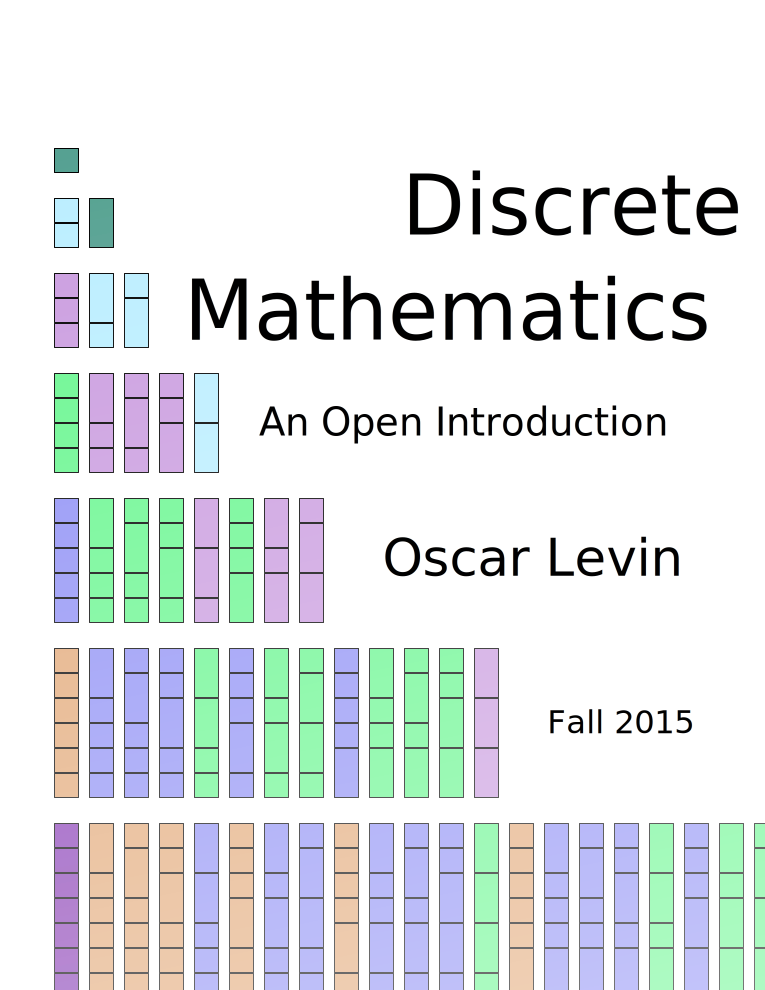
\includepdf[pages=-,pagecommand={\thispagestyle{empty}}]{frontmatter/cover2}
%
%

\clearpage






%\addtocontents{toc}{\protect\thispagestyle{plain}}

%% end: title page
%% begin: copyright-page
\thispagestyle{empty}
\vskip 3em

\noindent Oscar Levin \\ School of Mathematical Science \\ University of Northern Colorado \\ Greely, Co 80639 \\ \nolinkurl{oscar.levin@unco.edu} \\ \url{http://math.oscarlevin.com/}

\vfill
\vfill

\noindent\textcopyright ~ 2013-2016 by Oscar Levin

\vskip 3em

\noindent\includegraphics[scale=.5]{frontmatter/by-sa}\\
This work is licensed under the Creative Commons Attribution-ShareAlike 4.0 International License. To view a copy of this license, visit \url{http://creativecommons.org/licenses/by-sa/4.0/}.

\vskip 3em

\noindent Fall 2015 Edition
\vskip 1em
\noindent ISBN-10: 1516921186\\
\noindent ISBN-13: 978-1516921188
\vfill

\noindent A current version can always be found for free at \url{http://discretetext.oscarlevin.com/}
\vskip 2em

\noindent Cover image: \emph{Tiling with Fibonacci and Pascal}.
\clearpage

\vskip 2em
%% end:   copyright-page
%% begin: dedication-page
\cleardoublepage
\thispagestyle{empty}
\vspace*{\stretch{1}}
\begin{flushright}\large%
For Madeline and Teagan%
\end{flushright}
\vspace*{\stretch{2}}
\clearpage
%% end:   dedication-page
%% begin: obverse-dedication-page (empty)
\thispagestyle{empty}
\null%
\clearpage
%% end:   obverse-dedication-page
%% begin: acknowledgement
\chapter*{Acknowledgements}\label{acknowledgement-1}
\addcontentsline{toc}{chapter}{Acknowledgements}
\hypertarget{p-2}{}%
This book would not exist if not for ``Discrete and Combinatorial Mathematics'' by Richard Grassl and Tabitha Mingus. It is the book I learned discrete math out of, and taught out of the semester before I began writing this text. I wanted to maintain the inquiry based feel of their book but update, expand and rearrange some of the material.  Some of the best exposition and exercises here were graciously donated from this source.%
\par
\hypertarget{p-3}{}%
Thanks to Alees Seehausen who co-taught the Discrete Mathematics course with me in 2015 and helped develop many of the \emph{Investigate!} activities and other problems currently used in the text. She also offered many suggestions for improvement of the expository text, for which I am quite grateful. Thanks also to Katie Morrison and Nate Eldredge for their suggestions after using parts of this text in their class.%
\par
\hypertarget{p-4}{}%
While odds are that there are still errors and typos in the current book, there are many fewer thanks to the work of Michelle Morgan over the summer of 2016.%
\par
\hypertarget{p-5}{}%
The book is now available in an interactive online format, and this is entirely thanks to the work of Rob Beezer and David Farmer along with the rest of the participants of the \href{https://groups.google.com/forum/\#!forum/pretext-support}{pretext-support group}.%
\par
\hypertarget{p-6}{}%
Finally, a thank you to the numerous students who have pointed out typos and made suggestions over the years and a thanks in advance to those who will do so in the future.%
%% end:   acknowledgement
%% begin: preface
\chapter*{Preface}\label{preface}
\addcontentsline{toc}{chapter}{Preface}
\hypertarget{p-7}{}%
This text aims to give an introduction to select topics in discrete mathematics at a level appropriate for first or second year undergraduate math majors, especially those who intend to teach middle and high school mathematics. The book began as a set of notes for the Discrete Mathematics course at the University of Northern Colorado. This course serves both as a survey of the topics in discrete math and as the ``bridge'' course for math majors, as UNC does not offer a separate ``introduction to proofs'' course. Most students who take the course plan to teach, although there are a handful of students who will go on to graduate school or study applied math or computer science. For these students the current text hopefully is still of interest, but the intent is not to provide a solid mathematical foundation for computer science, unlike the majority of textbooks on the subject.%
\par
\hypertarget{p-8}{}%
Another difference between this text and most other discrete math books is that this book is intended to be used in a class taught using problem oriented or inquiry based methods. When I teach the class, I will assign sections for reading \emph{after} first introducing them in class by using a mix of group work and class discussion on a few interesting problems. The text is meant to consolidate what we \emph{discover} in class and serve as a reference for students as they master the concepts and techniques covered in the unit. None-the-less, every attempt has been made to make the text sufficient for self study as well, in a way that hopefully mimics an inquiry based classroom.%
\par
\hypertarget{p-9}{}%
The topics covered in this text were chosen to match the needs of the students I teach at UNC. The main areas of study are combinatorics, sequences, logic and proofs, and graph theory, in that order. Induction is covered at the end of the chapter on sequences. Most discrete books put logic first as a preliminary, which certainly has its advantages. However, I wanted to discuss logic and proofs together, and found that doing both of these before anything else was overwhelming for my students given that they didn't yet have context of other problems in the subject. Also, after spending a couple weeks on proofs, we would hardly use that at all when covering combinatorics, so much of the progress we made was quickly lost.  Instead, there is a short introduction section on mathematical statements, which should provide enough common language to discuss the logical content of combinatorics and sequences.%
\par
\hypertarget{p-10}{}%
Depending on the speed of the class, it might be possible to include additional material. In past semesters I have included generating functions (after sequences) and some basic number theory (either after the logic and proofs chapter or at the very end of the course). These additional topics are covered in the last chapter.%
\par
\hypertarget{p-11}{}%
While I (currently) believe this selection and order of topics is optimal, you should feel free to skip around to what interests you. There are occasionally examples and exercises that rely on earlier material, but I have tried to keep these to a minimum and usually can either be skipped or understood without too much additional study. If you are an instructor, feel free to edit the \LaTeX{} or Mathbook XML source to fit your needs.%
\typeout{************************************************}
\typeout{Paragraphs  Previous and future editions}
\typeout{************************************************}
\paragraph[{Previous and future editions}]{Previous and future editions}\hypertarget{pref_editions}{}
\hypertarget{p-12}{}%
This current 2nd edition brings a few major improvements, as well as \emph{lots} of minor corrections.  The highlights include: \leavevmode%
\begin{itemize}[label=\textbullet]
\item{}Some of the material from chapter 3 (on logic) is now part of an introduction section on mathematical statements.%
\item{}Content from the section on counting functions (previously 1.7) is now integrated with the rest of chapter 1.%
\item{}To accommodate instructors, some of the solutions to exercises were removed, and the more involved ``homework'' problems were integrated in the main exercises. New exercises and examples were added.  Currently there are about 360 exercises of which roughly 2/3 have solutions or answers.%
\item{}Behind the scenes, the source of the text transitioned from \LaTeX{} to Mathbook XML, which allows for conversion to \LaTeX{} as well as the creation of an interactive online version.%
\end{itemize}
%
\par
\hypertarget{p-13}{}%
The previous \emph{Fall 2015 edition} was essentially the first edition of the book. I had previously compiled many of the sections in a book format for easy distribution, but those were mostly just lecture notes and exercises (there was no index or Investigate problems; very little in the way of consistent formatting).%
\par
\hypertarget{p-14}{}%
My intent is to compile a new edition prior to each fall semester which incorporate additions and corrections suggested by instructors and students who use the text the previous semesters. Thus I encourage you to send along any suggestions and comments as you have them.%
\par\hfill\begin{tabular}{l@{}}
Oscar Levin, Ph.D.\\
University of Northern Colorado, 2016
\end{tabular}\\\par
%% end:   preface
%% begin: preface
\chapter*{How to use this book}\label{preface-2}
\addcontentsline{toc}{chapter}{How to use this book}
\hypertarget{p-15}{}%
In addition to expository text, this book has a few features designed to encourage you to interact with the mathematics.%
\typeout{************************************************}
\typeout{Paragraphs  \emph{Investigate!} activities}
\typeout{************************************************}
\paragraph[{\emph{Investigate!} activities}]{\emph{Investigate!} activities}\hypertarget{paragraphs-2}{}
\hypertarget{p-16}{}%
Sprinkled throughout the sections (usually at the very beginning of a topic) you will find activities designed to get you acquainted with the topic soon to be discussed. These are similar (sometimes identical) to group activities I give students to introduce material. You really should spend some time thinking about, or even working through, these problems before reading the section. By priming yourself to the types of issues involved in the material you are about to read, you will better understand what is to come. There are no solutions provided for these problems, but don't worry if you can't solve them or are not confident in your answers. My hope is that you will take this frustration with you while you read the proceeding section. By the time you are done with the section, things should be much clearer.%
\typeout{************************************************}
\typeout{Paragraphs  Examples}
\typeout{************************************************}
\paragraph[{Examples}]{Examples}\hypertarget{paragraphs-3}{}
\hypertarget{p-17}{}%
I have tried to include the ``correct'' number of examples. For those examples which include \emph{problems}, full solutions are included. Before reading the solution, try to at least have an understanding of what the problem is asking. Unlike some textbooks, the examples are not meant to be all inclusive for problems you will see in the exercises. They should not be used as a blueprint for solving other problems. Instead, use the examples to deepen our understanding of the concepts and techniques discussed in each section. Then use this understanding to solve the exercises at the end of each section.%
\typeout{************************************************}
\typeout{Paragraphs  Exercises}
\typeout{************************************************}
\paragraph[{Exercises}]{Exercises}\hypertarget{paragraphs-4}{}
\hypertarget{p-18}{}%
You get good at math through practice. Each section concludes with a small number of exercises meant to solidify concepts and basic skills presented in that section. At the end of each chapter, a larger collection of similar exercises is included (as a sort of ``chapter review'') which might bridge material of different sections in that chapter. Many exercise have a hint, answer or full solution (which in the pdf version of the text can be found by clicking on the exercises number\textemdash{}clicking on the solution number will bring you back to the exercise). Readers are encouraged to try these exercises before looking at the solution. When I teach with this book, I assign these exercises as practice and then use them, or similar problems, on quizzes and exams.  There are also problems without answers to challenge yourself (or to be assigned as homework).%
%% end:   preface
%% begin: table of contents
%% Adjust Table of Contents
\setcounter{tocdepth}{2}
\renewcommand*\contentsname{Contents}
\tableofcontents
%% end:   table of contents
\mainmatter
\typeout{************************************************}
\typeout{Chapter 0 Introduction and Preliminaries}
\typeout{************************************************}
\chapter[{Introduction and Preliminaries}]{Introduction and Preliminaries}\label{ch_intro}
\hypertarget{p-19}{}%
Welcome to Discrete Mathematics. If this is your first time encountering the subject, you will probably find discrete mathematics quite different from other math subjects. You might not even know what discrete math is! Hopefully this short introduction will shed some light on what the subject is about and what you can expect as you move forward in your studies.%
\typeout{************************************************}
\typeout{Section 0.1 What is Discrete Mathematics?}
\typeout{************************************************}
\section[{What is Discrete Mathematics?}]{What is Discrete Mathematics?}\label{sec_intro-intro}
\begin{quote}\hypertarget{blockquote-1}{}
\hypertarget{p-20}{}%
dis\textperiodcentered{}crete / dis'krët.%
\par
\hypertarget{p-21}{}%
\emph{Adjective}: Individually separate and distinct.%
\par
\hypertarget{p-22}{}%
\emph{Synonyms}: separate - detached - distinct - abstract.%
\end{quote}
\hypertarget{p-23}{}%
Defining \emph{discrete mathematics} is hard because defining \emph{mathematics} is hard. What is mathematics? The study of numbers? In part, but you also study functions and lines and triangles and parallelepipeds and vectors and \textellipsis{}. Or perhaps you want to say that mathematics is a collection of tools that allow you to solve problems. What sort of problems? Okay, those that involve numbers, functions, lines, triangles, \textellipsis{}. Whatever your conception of what mathematics is, try applying the concept of ``discrete'' to it, as defined above. Some math fundamentally deals with \emph{stuff} that is individually separate and distinct.%
\par
\hypertarget{p-24}{}%
In an algebra or calculus class, you might have found a particular set of numbers (maybe the set of numbers in the range of a function). You would represent this set as an interval: \([0,\infty)\) is the range of \(f(x) = x^2\) since the set of outputs of the function are all real numbers 0 and greater. This set of numbers is NOT discrete. The numbers in the set are not separated by much at all. In fact, take any two numbers in the set and there are infinitely many more between them which are also in the set. Discrete math could still ask about the range of a function, but the set would not be an interval. Consider the function which gives the number of children of each person reading this. What is the range? I'm guessing it is something like \(\{0, 1, 2, 3\}\). Maybe 4 is in there too. But certainly there is nobody reading this that has 1.32419 children. This set \emph{is} discrete because the elements are separate. Also notice that the inputs to the function are a discrete set as each input is an individual person. You would not consider fractional inputs (we don't care about anything \(2/3\) between a pair of readers).%
\par
\hypertarget{p-25}{}%
One way to get a feel for the subject is to consider the types of problems you solve in discrete math. Here are a few simple examples:%
\begin{investigation}[]\label{investigation-1}
\hypertarget{p-26}{}%
\emph{Note: Throughout the text you will see \emph{Investigate!} activities like this one. Answer the questions in these as best you can to give yourself a feel for what is coming next.}%
\par
\hypertarget{p-27}{}%
%
\begin{enumerate}
\item\hypertarget{li-5}{}\hypertarget{p-28}{}%
The most popular mathematician in the world is throwing a party for all of his friends. As a way to kick things off, they decide that everyone should shake hands. Assuming all 10 people at the party each shake hands with every other person (but not themselves, obviously) exactly once, how many handshakes take place?%
\item\hypertarget{li-6}{}\hypertarget{p-29}{}%
At the warm-up event for Oscar's All Star Hot Dog Eating Contest, Al ate one hot dog. Bob then showed him up by eating three hot dogs. Not to be outdone, Carl ate five. This continued with each contestant eating two more hot dogs than the previous contestant. How many hot dogs did Zeno (the 26th and final contestant) eat? How many hot dogs were eaten all together?%
\item\hypertarget{li-7}{}\hypertarget{p-30}{}%
After excavating for weeks, you finally arrive at the burial chamber. The room is empty except for two large chests. On each is carved a message (strangely in English):%
\begin{sidebyside}{1}{0.1}{0.1}{0}
\begin{sbspanel}{0.8}
\resizebox{\linewidth}{!}{{
\begin{tikzpicture}
          \node[shape=rectangle, draw=brown, thick, fill=brown!20!white, inner sep=5mm, minimum height=3cm, minimum width=3.5cm, text width=3.5cm, align=center] (a) { If this chest is empty, then the other chest's message is true.};
          \node[shape=rectangle, draw=brown, thick, fill=brown!20!white, inner sep=5mm, minimum height=3cm, minimum width=3.5cm, text width=3.5cm, align=center, right=of a] {
               This chest is filled with treasure or the other chest contains deadly scorpions.
              };
      \end{tikzpicture}
}
}
\end{sbspanel}
\end{sidebyside}
\par
\hypertarget{p-31}{}%
You know exactly one of these messages is true. What should you do?%
\item\hypertarget{li-8}{}\hypertarget{p-32}{}%
Back in the days of yore, five small towns decided they wanted to build roads directly connecting each pair of towns. While the towns had plenty of money to build roads as long and as winding as they wished, it was very important that the roads not intersect with each other (as stop signs had not yet been invented). Also, tunnels and bridges were not allowed. Is it possible for each of these towns to build a road to each of the four other towns without creating any intersections?%
\end{enumerate}
%
\end{investigation}
\hypertarget{p-33}{}%
One reason it is difficult to define discrete math is that it is a very broad description which encapsulates a large number of subjects. In this course we will study four main topics: \terminology{combinatorics} (the theory of ways things \emph{combine}; in particular, how to count these ways), \terminology{sequences}, \terminology{symbolic logic}, and \terminology{graph theory}. However, there are other topics that belong under the discrete umbrella, including computer science, abstract algebra, number theory, game theory, probability, and geometry (some of these, particularly the last two, have both discrete and non-discrete variants).%
\par
\hypertarget{p-34}{}%
Ultimately the best way to learn what discrete math is about is to \emph{do} it. Let's get started! Before we can begin answering more complicated (and fun) problems, we must lay down some foundation. We start by reviewing mathematical statements, sets, and functions in the framework of discrete mathematics.%
\typeout{************************************************}
\typeout{Section 0.2 Mathematical Statements}
\typeout{************************************************}
\section[{Mathematical Statements}]{Mathematical Statements}\label{sec_intro-statements}
\begin{investigation}[]\label{investigation-2}
\hypertarget{p-35}{}%
While walking through a fictional forest, you encounter three trolls guarding a bridge. Each is either a \emph{knight}, who always tells the truth, or a \emph{knave}, who always lies. The trolls will not let you pass until you correctly identify each as either a knight or a knave. Each troll makes a single statement:%
\begin{quote}\hypertarget{blockquote-2}{}
\hypertarget{p-36}{}%
Troll 1: If I am a knave, then there are exactly two knights here.%
\par
\hypertarget{p-37}{}%
Troll 2: Troll 1 is lying.%
\par
\hypertarget{p-38}{}%
Troll 3: Either we are all knaves or at least one of us is a knight.%
\end{quote}
\hypertarget{p-39}{}%
Which troll is which? \index{self reference|see{reference, self}} \index{reference, self|see{self reference}}%
\end{investigation}
\hypertarget{p-40}{}%
In order to \emph{do} mathematics, we must be able to \emph{talk} and \emph{write} about mathematics. Perhaps your experience with mathematics so far has mostly involved finding answers to problems. As we embark towards more advanced and abstract mathematics, writing will play a more prominent role in the mathematical process.%
\par
\hypertarget{p-41}{}%
Communication in mathematics requires more precision than many other subjects, and thus we should take a few pages here to consider the basic building blocks: \emph{mathematical statements}.%
\typeout{************************************************}
\typeout{Subsection  Atomic and Molecular Statements}
\typeout{************************************************}
\subsection[{Atomic and Molecular Statements}]{Atomic and Molecular Statements}\label{atomic-molecular-statements}
\hypertarget{p-42}{}%
A \terminology{statement}\index{statement} is any declarative sentence which is either true or false. A statement is \terminology{atomic} if it cannot be divided into smaller statements, otherwise it is called \terminology{molecular}.%
\begin{example}[]\label{example-1}
\hypertarget{p-43}{}%
These are statements (in fact, \emph{atomic} statements): \leavevmode%
\begin{itemize}[label=\textbullet]
\item{}\hypertarget{p-44}{}%
Telephone numbers in the USA have 10 digits.%
\item{}\hypertarget{p-45}{}%
The moon is made of cheese.%
\item{}\hypertarget{p-46}{}%
42 is a perfect square.%
\item{}\hypertarget{p-47}{}%
Every even number greater than 2 can be expressed as the sum of two primes.%
\item{}\hypertarget{p-48}{}%
\(3+7 = 12\)%
\end{itemize}
 And these are not statements: \leavevmode%
\begin{itemize}[label=\textbullet]
\item{}\hypertarget{p-49}{}%
Would you like some cake?%
\item{}\hypertarget{p-50}{}%
The sum of two squares.%
\item{}\(1+3+5+7+\cdots+2n+1\).%
\item{}\hypertarget{p-51}{}%
Go to your room!%
\item{}\hypertarget{p-52}{}%
\(3+x = 12\)%
\end{itemize}
%
\end{example}
\hypertarget{p-53}{}%
The reason the sentence ``\(3 + x = 12\)'' is not a statement is that it contains a variable. Depending on what \(x\) is, the sentence is either true or false, but right now it is neither. One way to make the \emph{sentence} into a \emph{statement} is to specify the value of the variable in some way. This could be done by specifying a specific substitution, for example, ``\(3+x = 12\) where \(x = 9\),'' which is a true statement.  Or you could \emph{capture} the free variable by \emph{quantifying} over it, as in, ``for all values of \(x\), \(3+x = 12\),'' which is false. We will discuss quantifiers in more detail at the end of this section.%
\par
\hypertarget{p-54}{}%
You can build more complicated (molecular) statements out of simpler (atomic or molecular) ones using \terminology{logical connectives} \index{connectives}. For example, this is a molecular statement:%
\begin{quote}\hypertarget{blockquote-3}{}
\hypertarget{p-55}{}%
Telephone numbers in the USA have 10 digits and 42 is a perfect square.%
\end{quote}
\hypertarget{p-56}{}%
Note that we can break this down into two smaller statements. The two shorter statements are \emph{connected} by an ``and.'' We will consider 5 connectives: ``and'' (Sam is a man and Chris is a woman), ``or'' (Sam is a man or Chris is a woman), ``if\textellipsis{}, then\textellipsis{}'' (if Sam is a man, then Chris is a woman), ``if and only if'' (Sam is a man if and only if Chris is a woman), and ``not'' (Sam is not a man). The first four are called \terminology{binary connectives} (because they connect two statements) while ``not'' is an example of a \terminology{unary connective} (since it applies to a single statement).%
\par
\hypertarget{p-57}{}%
These molecular statements are of course still statements, so they must be either true or false.  The absolutely key observation here is that which \terminology{truth value} \index{truth value} the molecular statement achieves is completely determined by the type of connective and the truth values of the parts. We do not need to know what the parts actually say, only whether those parts are true or false. So to analyze logical connectives, it is enough to consider \terminology{propositional variables} (sometimes called \emph{sentential} variables), usually capital letters in the middle of the alphabet: \(P, Q, R, S, \ldots\).  We think of these as standing in for (usually atomic) statements, but there are only two \emph{values} the variables can achieve: true or false.\footnote{In computer programing, we should call such variables \terminology{Boolean variables}.\label{fn-1}} \label{notation-1}
 We also have symbols for the logical connectives: \(\wedge\), \(\vee\), \(\imp\), \(\iff\), \(\neg\).%
\begin{assemblage}[Logical Connectives]\label{assemblage-1}
\hypertarget{p-58}{}%
%
\begin{itemize}[label=\textbullet]
\item{}\(P \wedge Q\) is read ``\(P\) and \(Q\),'' and called a \terminology{conjunction}. \index{conjunction} \index{connectives!and}\label{notation-2}
%
\item{}\(P \vee Q\) is read ``\(P\) or \(Q\),'' and called a \terminology{disjunction}. \index{disjunction} \index{connectives!or}\label{notation-3}
%
\item{}\(P \imp Q\) is read ``if \(P\) then \(Q\),'' and called an \terminology{implication} or \terminology{conditional}. \index{implication} \index{conditional} \index{connectives!implies} \index{if\textellipsis{}, then\textellipsis{}}%
\item{}\(P \iff Q\) is read ``\(P\) if and only if \(Q\),'' and called a \terminology{biconditional}. \index{biconditional} \index{connectives!if and only if} \index{if and only if}%
\item{}\(\neg P\) is read ``not \(P\),'' and called a \terminology{negation}. \index{negation} \index{connectives!not}\label{notation-4}
%
\end{itemize}
%
\end{assemblage}
\hypertarget{p-59}{}%
The \terminology{truth value} of a statement is determined by the truth value(s) of its part(s), depending on the connectives:%
\begin{assemblage}[Truth Conditions for Connectives]\label{assemblage-2}
\hypertarget{p-60}{}%
%
\begin{itemize}[label=\textbullet]
\item{}\(P \wedge Q\) is true when both \(P\) and \(Q\) are true%
\item{}\(P \vee Q\) is true when \(P\) or \(Q\) or both are true.%
\item{}\(P \imp Q\) is true when \(P\) is false or \(Q\) is true or both.%
\item{}\(P \iff Q\) is true when \(P\) and \(Q\) are both true, or both false.%
\item{}\(\neg P\) is true when \(P\) is false.%
\end{itemize}
%
\end{assemblage}
\hypertarget{p-61}{}%
Note that for us, \emph{or} is the \terminology{inclusive or} \index{inclusive or} (and not the sometimes used \emph{exclusive or}) meaning that \(P \vee Q\) is in fact true when both \(P\) and \(Q\) are true. As for the other connectives, ``and'' behaves as you would expect, as does negation. The biconditional (if and only if) might seem a little strange, but you should think of this as saying the two parts of the statements are \emph{equivalent} in that they have the same truth value. This leaves only the conditional \(P \imp Q\) which has a slightly different meaning in mathematics than it does in ordinary usage. However, implications are so common and useful in mathematics, that we must develop fluency with their use, and as such, they deserve their own subsection.%
\typeout{************************************************}
\typeout{Subsection  Implications}
\typeout{************************************************}
\subsection[{Implications}]{Implications}\label{subsec_implications}
\begin{assemblage}[Implications]\label{assemblage-3}
\hypertarget{p-62}{}%
An \terminology{implication} or \terminology{conditional} is a molecular statement of the form%
\begin{equation*}
P \imp Q
\end{equation*}
where \(P\) and \(Q\) are statements.  We say that %
\begin{itemize}[label=\textbullet]
\item{}\(P\) is the \terminology{hypothesis} (or \terminology{antecedent}).%
\item{}\(Q\) is the \terminology{conclusion} (or \terminology{consequent}).%
\end{itemize}
%
\par
\hypertarget{p-63}{}%
An implication is \emph{true} provided \(P\) is false or  \(Q\) is true (or both), and \emph{false} otherwise.  In particular, the only way for \(P \imp Q\) to be false is for \(P\) to be true \emph{and} \(Q\) to be false.%
\end{assemblage}
\hypertarget{p-64}{}%
Easily the most common type of statement in mathematics is the implication. Even statements that do not at first look like they have this form conceal an implication at their heart. Consider the \emph{Pythagorean Theorem}. Many a college freshman would quote this theorem as ``\(a^2 + b^2 = c^2\).'' This is absolutely not correct. For one thing, that is not a statement since it has three variables in it. Perhaps they imply that this should be true for any values of the variables?  So \(1^2 + 5^2 = 2^2\)??? How can we fix this? Well, the equation is true as long as \(a\) and \(b\) are the legs or a right triangle and \(c\) is the hypotenuse. In other words:%
\begin{quote}\hypertarget{blockquote-4}{}
\hypertarget{p-65}{}%
\emph{If} \(a\) and \(b\) are the legs of a right triangle with hypotenuse \(c\), \emph{then} \(a^2 + b^2 = c^2\).%
\end{quote}
\hypertarget{p-66}{}%
This is a reasonable way to think about implications: our claim is that the conclusion (``then'' part) is true, but on the assumption that the hypothesis (``if'' part) is true. We make no claim about the conclusion in situations when the hypothesis is false.\footnote{However, note that in the case of the Pythagorean Theorem, it is also the case that \emph{if} \(a^2 + b^2 = c^2\), \emph{then} \(a\) and \(b\) are the legs of a right triangle with hypotenuse \(c\).  So we could have also expressed this theorem as a biconditional: ``\(a\) and \(b\) are the legs of a right triangle with hypotenuse \(c\) \emph{if and only if} \(a^2 + b^2 = c^2\).''\label{fn-2}}%
\par
\hypertarget{p-67}{}%
Still, it is important to remember that an implication is a statement, and therefore is either true or false. The truth value of the implication is determined by the truth values of its two parts. To agree with the usage above, we say that an implication is true either when the hypothesis is false, or when the conclusion is true. This leaves only one way for an implication to be false: when the hypothesis is true and the conclusion is false.%
\begin{example}[]\label{example-2}
\hypertarget{p-68}{}%
Consider the statement:%
\begin{quote}\hypertarget{blockquote-5}{}
\hypertarget{p-69}{}%
If Bob gets a 90 on the final, then Bob will pass the class.%
\end{quote}
\hypertarget{p-70}{}%
This is definitely an implication: \(P\) is the statement ``Bob gets a 90 on the final,'' and \(Q\) is the statement ``Bob will pass the class.''%
\par
\hypertarget{p-71}{}%
Suppose I made that statement to Bob. In what circumstances would it be fair to call me a liar? What if Bob really did get a 90 on the final, and he did pass the class? Then I have not lied; my statement is true. However, if Bob did get a 90 on the final and did not pass the class, then I lied, making the statement false. The tricky case is this: what if Bob did not get a 90 on the final? Maybe he passes the class, maybe he doesn't. Did I lie in either case? I think not. In these last two cases, \(P\) was false, and the statement \(P \imp Q\) was true. In the first case, \(Q\) was true, and so was \(P \imp Q\). So \(P \imp Q\) is true when either \(P\) is false or \(Q\) is true.%
\end{example}
\hypertarget{p-72}{}%
Just to be clear, although we sometimes read \(P \imp Q\) as ``\(P\) \emph{implies} \(Q\)'', we are not insisting that there is some causal relationship between the statements \(P\) and \(Q\). In particular, if you claim that \(P \imp Q\) is \emph{false}, you are not saying that \(P\) does not imply \(Q\), but rather that \(P\) is true and \(Q\) is false.%
\begin{example}[]\label{example-3}
\hypertarget{p-73}{}%
Decide which of the following statements are true and which are false. Briefly explain. \leavevmode%
\begin{enumerate}
\item\hypertarget{li-31}{}\hypertarget{p-74}{}%
If \(1=1\), then most horses have 4 legs.%
\item\hypertarget{li-32}{}\hypertarget{p-75}{}%
If \(0=1\), then \(1=1\).%
\item\hypertarget{li-33}{}\hypertarget{p-76}{}%
If 8 is a prime number, then the 7624th digit of \(\pi\) is an 8.%
\item\hypertarget{li-34}{}\hypertarget{p-77}{}%
If the 7624th digit of \(\pi\) is an 8, then \(2+2 = 4\).%
\end{enumerate}
%
\par\smallskip%
\noindent\textbf{Solution.}\hypertarget{solution-1}{}\quad%
\hypertarget{p-78}{}%
All four of the statements are true. Remember, the only way for an implication to be false is for the \emph{if} part to be true and the \emph{then} part to be false. \leavevmode%
\begin{enumerate}
\item\hypertarget{li-35}{}\hypertarget{p-79}{}%
Here both the hypothesis and the conclusion are true, so the implication is true. It does not matter that there is no meaningful connection between the true mathematical fact and the fact about horses.%
\item\hypertarget{li-36}{}\hypertarget{p-80}{}%
Here the hypothesis is false and the conclusion is true, so the implication is true.%
\item\hypertarget{li-37}{}\hypertarget{p-81}{}%
I have no idea what the 7624th digit of \(\pi\) is, but this does not matter. Since the hypothesis is false, the implication is automatically true.%
\item\hypertarget{li-38}{}\hypertarget{p-82}{}%
Similarly here, regardless of the truth value of the hypothesis, the conclusion is true, making the implication true.%
\end{enumerate}
%
\end{example}
\hypertarget{p-83}{}%
It is important to understand the conditions under which an implication is true not only to decide whether a mathematical statement is true, but in order to \emph{prove} that it is. Proofs might seem scary (especially if you have had a bad high school geometry experience) but all we are really doing is explaining (very carefully) why a statement is true. If you understand the truth conditions for an implication, you already have the outline for a proof.%
\begin{assemblage}[Direct Proofs of Implications]\label{assemblage-4}
\hypertarget{p-84}{}%
To prove an implication \(P \imp Q\), it is enough to assume \(P\), and from it, deduce \(Q\).%
\end{assemblage}
\hypertarget{p-85}{}%
Perhaps a better way to say this is that to prove a statement of the form \(P \imp Q\) directly, you must explain why \(Q\) is true, but you \emph{get to} assume \(P\) is true first.  After all, you only care about whether \(Q\) is true in the case that \(P\) is as well.%
\par
\hypertarget{p-86}{}%
There are other techniques to prove statements (implications and others) that we will encounter throughout our studies, and new proof techniques are discovered all the time. Direct proof is the easiest and most elegant style of proof and has the advantage that such a proof often does a great job of explaining \emph{why} the statement is true.%
\begin{example}[]\label{example-4}
\hypertarget{p-87}{}%
Prove: If two numbers \(a\) and \(b\) are even, then their sum \(a+b\) is even.%
\par\smallskip%
\noindent\textbf{Solution.}\hypertarget{solution-2}{}\quad%
\begin{proof}\hypertarget{proof-1}{}
\hypertarget{p-88}{}%
Suppose the numbers \(a\) and \(b\) are even. This means that  \(a = 2k\) and \(b=2j\) for some integers \(k\) and \(j\). The sum is then \(a+b = 2k+2j = 2(k+j)\). Since \(k+j\) is an integer, this means that \(a+b\) is even.%
\end{proof}
\hypertarget{p-89}{}%
Notice that since we get to assume the hypothesis of the implication we immediately have a place to start. The proof proceeds essentially by repeatedly asking and answering, ``what does that mean?''  Eventually, we conclude that the means the conclusion.%
\end{example}
\hypertarget{p-90}{}%
This sort of argument shows up outside of math as well. If you ever found yourself starting an argument with ``hypothetically, let's assume \textellipsis{},'' then you have attempted a direct proof of your desired conclusion.%
\par
\hypertarget{p-91}{}%
An implication is a way of expressing a relationship between two statements.  It is often interesting to ask whether there are other relationships between the statements.  Here we introduce some common language to address this question.%
\begin{assemblage}[Converse and Contrapositive]\label{assemblage-5}
\hypertarget{p-92}{}%
%
\begin{itemize}[label=\textbullet]
\item{}\hypertarget{p-93}{}%
The \terminology{converse} \index{converse} of an implication \(P \imp Q\) is the implication \(Q \imp P\). The converse is NOT logically equivalent to the original implication.  That is, whether the converse of an implication is true is independent of the truth of the implication.%
\item{}\hypertarget{p-94}{}%
The \terminology{contrapositive} \index{contrapositive} of an implication \(P \imp Q\) is the statement \(\neg Q \imp \neg P\). An implication and its contrapositive are logically equivalent (they are either both true or both false).%
\end{itemize}
%
\end{assemblage}
\hypertarget{p-95}{}%
Mathematics is overflowing with examples of true implications which have a false converse. If a number greater than 2 is prime, then that number is odd. However, just because a number is odd does not mean it is prime. If a shape is a square, then it is a rectangle. But it is false that if a shape is a rectangle, then it is a square. While this happens often, it does not always happen. For example, the Pythagorean theorem has a true converse: if\(a^2 + b^2 = c^2\), then the triangle with sides \(a\), \(b\), and \(c\) is a \emph{right} triangle. Whenever you encounter an implication in mathematics, it is always reasonable to ask whether the converse is true.%
\par
\hypertarget{p-96}{}%
The contrapositive, on the other hand, always has the same truth value as its original implication. This can be very helpful in deciding whether an implication is true: often it is easier to analyze the contrapositive.%
\begin{example}[]\label{example-5}
\hypertarget{p-97}{}%
True or false: If you draw any nine playing cards from a regular deck, then you will have at least three cards all of the same suit. Is the converse true?%
\par\smallskip%
\noindent\textbf{Solution.}\hypertarget{solution-3}{}\quad%
\hypertarget{p-98}{}%
True. The original implication is a little hard to analyze because there are so many different combinations of nine cards. But consider the contrapositive: If you \emph{don't} have at least three cards all of the same suit, then you don't have nine cards. It is easy to see why this is true: you can at most have two cards of each of the four suits, for a total of eight cards (or fewer).%
\par
\hypertarget{p-99}{}%
The converse: If you have at least three cards all of the same suit, then you have nine cards. This is false. You could have three spades and nothing else. Note that to demonstrate that the converse (an implication) is false, we provided an example where the hypothesis is true (you do have three cards of the same suit), but where the conclusion is false (you do not have nine cards).%
\end{example}
\hypertarget{p-100}{}%
Understanding converses and contrapositives can help understand implications and their truth values:%
\begin{example}[]\label{example-6}
\hypertarget{p-101}{}%
Suppose I tell Sue that if she gets a 93\% on her final, then she will get an A in the class. Assuming that what I said is true, what can you conclude in the following cases:%
\par
\hypertarget{p-102}{}%
\leavevmode%
\begin{enumerate}
\item\hypertarget{li-41}{}\hypertarget{p-103}{}%
Sue gets a 93\% on her final.%
\item\hypertarget{li-42}{}\hypertarget{p-104}{}%
Sue gets an A in the class.%
\item\hypertarget{li-43}{}\hypertarget{p-105}{}%
Sue does not get a 93\% on her final.%
\item\hypertarget{li-44}{}\hypertarget{p-106}{}%
Sue does not get an A in the class.%
\end{enumerate}
%
\par\smallskip%
\noindent\textbf{Solution.}\hypertarget{solution-4}{}\quad%
\hypertarget{p-107}{}%
Note first that whenever \(P \imp Q\) and \(P\) are both true statements, \(Q\) must be true as well. For this problem, take \(P\) to mean ``Sue gets a 93\% on her final'' and \(Q\) to mean ``Sue will get an A in the class.''%
\par
\hypertarget{p-108}{}%
\leavevmode%
\begin{enumerate}
\item\hypertarget{li-45}{}\hypertarget{p-109}{}%
We have \(P \imp Q\) and \(P\), so \(Q\) follows. Sue gets an A.%
\item\hypertarget{li-46}{}\hypertarget{p-110}{}%
You cannot conclude anything. Sue could have gotten the A because she did extra credit for example. Notice that we do not know that if Sue gets an \(A\), then she gets a 93\% on her final. That is the converse of the original implication, so it might or might not be true.%
\item\hypertarget{li-47}{}\hypertarget{p-111}{}%
The contrapositive of the converse of \(P \imp Q\) is \(\neg P \imp \neg Q\), which states that if Sue does not get a 93\% on the final, then she will not get an A in the class. But this does not follow from the original implication. Again, we can conclude nothing. Sue could have done extra credit.%
\item\hypertarget{li-48}{}\hypertarget{p-112}{}%
What would happen if Sue does not get an A but \emph{did} get a 93\% on the final? Then \(P\) would be true and \(Q\) would be false. This makes the implication \(P \imp Q\) false! It must be that Sue did not get a 93\% on the final. Notice now we have the implication \(\neg Q \imp \neg P\) which is the contrapositive of \(P \imp Q\). Since \(P \imp Q\) is assumed to be true, we know \(\neg Q \imp \neg P\) is true as well.%
\end{enumerate}
%
\end{example}
\hypertarget{p-113}{}%
As we said above, an implication is not logically equivalent to its converse, but it is possible that both the implication and its converse are true. In this case, when both \(P \imp Q\) and \(Q \imp P\) are true, we say that \(P\) and \(Q\) are equivalent and write \(P \iff Q\). This is the biconditional we mentioned earlier.%
\begin{assemblage}[If and only if]\label{assemblage-6}
\begin{quote}\hypertarget{blockquote-6}{}
\hypertarget{p-114}{}%
\(P \iff Q\) is logically equivalent to \((P \imp Q) \wedge (Q \imp P)\).%
\end{quote}
\hypertarget{p-115}{}%
Example: Given an integer \(n\), it is true that \(n\) is even if and only if \(n^2\) is even. That is, if \(n\) is even, then \(n^2\) is even, as well as the converse: if \(n^2\) is even, then \(n\) is even.%
\end{assemblage}
\hypertarget{p-116}{}%
You can think of ``if and only if'' statements as having two parts: an implication and its converse. We might say one is the ``if'' part, and the other is the ``only if'' part. We also sometimes say that ``if and only if'' statements have two directions: a forward direction \((P \imp Q)\) and a backwards direction (\(P \leftarrow Q\), which is really just sloppy notation for \(Q \imp P\)).%
\par
\hypertarget{p-117}{}%
Let's think a little about which part is which. Is \(P \imp Q\) the ``if'' part or the ``only if'' part? Consider an example.%
\begin{example}[]\label{example-7}
\hypertarget{p-118}{}%
Suppose it is true that I sing if and only if I'm in the shower. We know this means both that if I sing, then I'm in the shower, and also the converse, that if I'm in the shower, then I sing. Let \(P\) be the statement, ``I sing,'' and \(Q\) be, ``I'm in the shower.'' So \(P \imp Q\) is the statement ``if I sing, then I'm in the shower.'' Which part of the if and only if statement is this?%
\par
\hypertarget{p-119}{}%
What we are really asking for is the meaning of ``I sing \emph{if} I'm in the shower'' and ``I sing \emph{only if} I'm in the shower.'' When is the first one (the ``if'' part) \emph{false}? When I am in the shower but not singing. That is the same condition on being false as the statement ``if I'm in the shower, then I sing.'' So the ``if'' part is \(Q \imp P\). On the other hand, to say, ``I sing only if I'm in the shower'' is equivalent to saying ``if I sing, then I'm in the shower,'' so the ``only if'' part is \(P \imp Q\).%
\end{example}
\hypertarget{p-120}{}%
It is not terribly important to know which part is the ``if'' or ``only if'' part, but this does illustrate something very, very important: \emph{there are many ways to state an implication!}%
\begin{example}[]\label{example-8}
\hypertarget{p-121}{}%
Rephrase the implication, ``if I dream, then I am asleep'' in as many different ways as possible. Then do the same for the converse.%
\par\smallskip%
\noindent\textbf{Solution.}\hypertarget{solution-5}{}\quad%
\hypertarget{p-122}{}%
The following are all equivalent to the original implication: \leavevmode%
\begin{enumerate}
\item\hypertarget{li-49}{}\hypertarget{p-123}{}%
I am asleep if I dream.%
\item\hypertarget{li-50}{}\hypertarget{p-124}{}%
I dream only if I am asleep.%
\item\hypertarget{li-51}{}\hypertarget{p-125}{}%
In order to dream, I must be asleep.%
\item\hypertarget{li-52}{}\hypertarget{p-126}{}%
To dream, it is necessary that I am asleep.%
\item\hypertarget{li-53}{}\hypertarget{p-127}{}%
To be asleep, it is sufficient to dream.%
\item\hypertarget{li-54}{}\hypertarget{p-128}{}%
I am not dreaming unless I am asleep.%
\end{enumerate}
 The following are equivalent to the converse (if I am asleep, then I dream): \leavevmode%
\begin{enumerate}
\item\hypertarget{li-55}{}\hypertarget{p-129}{}%
I dream if I am asleep.%
\item\hypertarget{li-56}{}\hypertarget{p-130}{}%
I am asleep only if I dream.%
\item\hypertarget{li-57}{}\hypertarget{p-131}{}%
It is necessary that I dream in order to be asleep.%
\item\hypertarget{li-58}{}\hypertarget{p-132}{}%
It is sufficient that I be asleep in order to dream.%
\item\hypertarget{li-59}{}\hypertarget{p-133}{}%
If I don't dream, then I'm not asleep.%
\end{enumerate}
%
\end{example}
\hypertarget{p-134}{}%
Hopefully you agree with the above example. We include the ``necessary and sufficient'' versions because those are common when discussing mathematics. In fact, let's agree once and for all what they mean.%
\begin{assemblage}[Necessary and Sufficient]\label{assemblage-7}
\hypertarget{p-135}{}%
\index{necessary condition} \index{sufficient condition}%
\par
\hypertarget{p-136}{}%
%
\begin{itemize}[label=\textbullet]
\item{}``\(P\) is necessary for \(Q\)'' means \(Q \imp P\).%
\item{}``\(P\) is sufficient for \(Q\)'' means \(P \imp Q\).%
\item{}\hypertarget{p-137}{}%
If \(P\) is necessary and sufficient for \(Q\), then \(P \iff Q\).%
\end{itemize}
%
\end{assemblage}
\hypertarget{p-138}{}%
To be honest, I have trouble with these if I'm not very careful. I find it helps to keep a standard example for reference.%
\begin{example}[]\label{example-9}
\hypertarget{p-139}{}%
Recall from calculus, if a function is differentiable at a point \(c\), then it is continuous at \(c\), but that the converse of this statement is not true (for example, \(f(x) = |x|\) at the point 0). Restate this fact using ``necessary and sufficient'' language.%
\par\smallskip%
\noindent\textbf{Solution.}\hypertarget{solution-6}{}\quad%
\hypertarget{p-140}{}%
It is true that in order for a function to be differentiable at a point \(c\), it is necessary for the function to be continuous at \(c\). However, it is not necessary that a function be differentiable at \(c\) for it to be continuous at \(c\).%
\par
\hypertarget{p-141}{}%
It is true that to be continuous at a point \(c\), it is sufficient that the function be differentiable at \(c\). However, it is not the case that being continuous at \(c\) is sufficient for a function to be differentiable at \(c\).%
\end{example}
\hypertarget{p-142}{}%
Thinking about the necessity and sufficiency of conditions can also help when writing proofs and justifying conclusions. If you want to establish some mathematical fact, it is helpful to think what other facts would \emph{be enough} (be sufficient) to prove your fact. If you have an assumption, think about what must also be necessary if that hypothesis is true.%
\typeout{************************************************}
\typeout{Subsection  Quantifiers}
\typeout{************************************************}
\subsection[{Quantifiers}]{Quantifiers}\label{subsec_quantifiers}
\begin{investigation}[]\label{investigation-3}
\hypertarget{p-143}{}%
Consider the statements below. Decide whether any are equivalent to each other, or whether any imply any others.%
\par
\hypertarget{p-144}{}%
%
\begin{enumerate}
\item\hypertarget{li-63}{}\hypertarget{p-145}{}%
You can fool some people all of the time.%
\item\hypertarget{li-64}{}\hypertarget{p-146}{}%
You can fool everyone some of the time.%
\item\hypertarget{li-65}{}\hypertarget{p-147}{}%
You can always fool some people.%
\item\hypertarget{li-66}{}\hypertarget{p-148}{}%
Sometimes you can fool everyone.%
\end{enumerate}
%
\end{investigation}
\hypertarget{p-149}{}%
It would be nice to use variables in our mathematical sentences. For example, suppose we wanted to claim that if \(n\) is prime, then \(n+7\) is not prime. This looks like an implication. I would like to write something like%
\begin{equation*}
P(n) \imp \neg P(n+7) 
\end{equation*}
where \(P(n)\) means ``\(n\) is prime.'' But this is not quite right. For one thing, because this sentence has a \terminology{free variable} (that is, a variable that we have not specified anything about), it is not a statement. Now, if we plug in a specific value for \(n\), we do get a statement. In fact, it turns out that no matter what value we plug in for \(n\), we get a true implication. What we really want to say is that \emph{for all} values of \(n\), if \(n\) is prime, then \(n+7\) is not. We need to \emph{quantify} the variable.%
\par
\hypertarget{p-150}{}%
Although there are many types of \emph{quantifiers} in English (e.g., many, few, most, etc.) in mathematics we, for the most part, stick to two: existential and universal.%
\begin{assemblage}[Universal and Existential Quantifiers]\label{assemblage-8}
\hypertarget{p-151}{}%
\index{quantifiers}%
\par
\hypertarget{p-152}{}%
The existential quantifier is \(\exists\) and is read ``there exists'' or ``there is.'' For example,\index{existential quantifier} \index{quantifiers!exists}\label{notation-5}
%
\begin{equation*}
\exists x (x \lt 0)
\end{equation*}
asserts that there is a number less than 0.%
\par
\hypertarget{p-153}{}%
The universal quantifier is \(\forall\) and is read ``for all'' or ``every.'' For example,\index{universal quantifier} \index{quantifiers!for all} \label{notation-6}
%
\begin{equation*}
\forall x (x \ge 0)
\end{equation*}
asserts that every number is greater than or equal to 0.%
\end{assemblage}
\hypertarget{p-154}{}%
As with all mathematical statements, we would like to decide whether quantified statements are true or false. Consider the statement%
\begin{equation*}
\forall x \exists y (y \lt x).
\end{equation*}
You would read this, ``for every \(x\) there is some \(y\) such that \(y\) is less than \(x\).'' Is this true? The answer depends on what our \emph{domain of discourse} is: when we say ``for all'' \(x\), do we mean all positive integers or all real numbers or all elements of some other set? Usually this information is implied. In discrete mathematics, we almost always quantify over the \emph{natural numbers}, 0, 1, 2, \textellipsis{}, so let's take that for our domain of discourse here.%
\par
\hypertarget{p-155}{}%
For the statement to be true, we need it to be the case that no matter what natural number we select, there is always some natural number that is strictly smaller. Perhaps we could let \(y\) be \(x-1\)? But here is the problem: what if \(x = 0\)? Then \(y = -1\) and that is \emph{not a number!} (in our domain of discourse). Thus we see that the statement is false because there is a number which is less than or equal to all other numbers. In symbols,%
\begin{equation*}
\exists x \forall y (y \ge x).
\end{equation*}
%
\par
\hypertarget{p-156}{}%
To show that the original statement is false, we proved that the \emph{negation} was true. Notice how the negation and original statement compare. This is typical.%
\begin{assemblage}[Quantifiers and Negation]\label{assemblage-9}
\begin{quote}\hypertarget{blockquote-7}{}
\hypertarget{p-157}{}%
\(\neg \forall x P(x)\) is equivalent to \(\exists x \neg P(x)\).%
\par
\hypertarget{p-158}{}%
\(\neg \exists x P(x)\) is equivalent to \(\forall x \neg P(x)\).%
\end{quote}
\end{assemblage}
\hypertarget{p-159}{}%
Essentially, we can pass the negation symbol over a quantifier, but that causes the quantifier to switch type. This should not be surprising: if not everything has a property, then something doesn't have that property. And if there is not something with a property, then everything doesn't have that property.%
\typeout{************************************************}
\typeout{Exercises  Practice}
\typeout{************************************************}
\subsection[{Practice}]{Practice}\label{practice_intro-statements}
\begin{exerciselist}
\item[1.]\hypertarget{exercise-1}{}\noindent%
\hypertarget{p-160}{}%
For each sentence below, decide whether it is an atomic statement, a molecular statement, or not a statement at all.%
\par
\hypertarget{p-161}{}%
\leavevmode%
\begin{enumerate}[label=(\alph*)]
\item\hypertarget{li-67}{}\hypertarget{p-162}{}%
Customers must wear shoes. (Choose one: atomic statement, molecular statement, or not a statement)%
\item\hypertarget{li-68}{}\hypertarget{p-163}{}%
The customers wore shoes. (Choose one: atomic statement, molecular statement, or not a statement)%
\item\hypertarget{li-69}{}\hypertarget{p-164}{}%
The customers wore shoes and socks. (Choose one: atomic statement, molecular statement, or not a statement)%
\end{enumerate}
%
\par
\medskip\noindent%
\textbf{Solution.}\quad \hypertarget{p-165}{}%
\leavevmode%
\begin{enumerate}[label=(\alph*)]
\item\hypertarget{li-70}{}\hypertarget{p-166}{}%
This is not a statement.  It is an imperative sentence, but is not either true or false.  It doesn't matter that this might actually be the rule or not.  Note that ``The rule is that all customers must wear shoes'' \emph{is} a statement.%
\item\hypertarget{li-71}{}\hypertarget{p-167}{}%
This is a statement, as it is either true or false.  It is an atomic statement because it cannot be divided into smaller statements.%
\item\hypertarget{li-72}{}\hypertarget{p-168}{}%
This is again a statement, but this time it is molecular.  In fact, it is a conjunction, as we can write it as ``The customers wore shoes and the customers wore socks.''%
\end{enumerate}
%
\par
\item[2.]\hypertarget{exercise-2}{}\noindent%
\hypertarget{p-169}{}%
Determine whether each molecular statement below is true or false, or whether it is impossible to determine.  Assume you do not know what my favorite number is (but you do know that 13 is prime).%
\par
\hypertarget{p-170}{}%
\leavevmode%
\begin{enumerate}[label=(\alph*)]
\item\hypertarget{li-73}{}\hypertarget{p-171}{}%
If 13 is prime, then 13 is my favorite number. (Choose one: True, False, or Not enough information)%
\item\hypertarget{li-74}{}\hypertarget{p-172}{}%
If 13 is my favorite number, then 13 is prime. (Choose one: True, False, or Not enough information)%
\item\hypertarget{li-75}{}\hypertarget{p-173}{}%
If 13 is not prime, then 13 is my favorite number. (Choose one: True, False, or Not enough information)%
\item\hypertarget{li-76}{}\hypertarget{p-174}{}%
13 is my favorite number or 13 is prime. (Choose one: True, False, or Not enough information)%
\item\hypertarget{li-77}{}\hypertarget{p-175}{}%
13 is my favorite number and 13 is prime. (Choose one: True, False, or Not enough information)%
\item\hypertarget{li-78}{}\hypertarget{p-176}{}%
7 is my favorite number and 13 is not prime. (Choose one: True, False, or Not enough information)%
\item\hypertarget{li-79}{}\hypertarget{p-177}{}%
13 is my favorite number or 13 is not my favorite number. (Choose one: True, False, or Not enough information)%
\end{enumerate}
%
\par
\medskip\noindent%
\textbf{Solution.}\quad \hypertarget{p-178}{}%
\leavevmode%
\begin{enumerate}[label=(\alph*)]
\item\hypertarget{li-80}{}\hypertarget{p-179}{}%
It is impossible to tell.  The hypothesis of the implication is true.  Thus the implication will be true if the conclusion is true (if 13 \emph{is} my favorite number) and false otherwise.%
\item\hypertarget{li-81}{}\hypertarget{p-180}{}%
This is true, no matter whether 13 is my favorite number or not.  Any implication with a true conclusion is true.%
\item\hypertarget{li-82}{}\hypertarget{p-181}{}%
This is true, again, no matter whether 13 is my favorite number or not.  Any implication with a false hypothesis is true.%
\item\hypertarget{li-83}{}\hypertarget{p-182}{}%
For a disjunction to be true, we just need one or the other (or both) of the parts to be true.  Thus this is a true statement.%
\item\hypertarget{li-84}{}\hypertarget{p-183}{}%
We cannot tell.  The statement would be true if 13 is my favorite number, and false if not (since a conjunction needs both parts to be true to be true).%
\item\hypertarget{li-85}{}\hypertarget{p-184}{}%
This is definitely false.  13 is prime, so its negation (13 is not prime) is false.  At least one part of the conjunction is false, so the whole statement is false.%
\item\hypertarget{li-86}{}\hypertarget{p-185}{}%
This is true.  Either 13 is my favorite number or it is not, but whichever it is, at least one part of the disjunction is true, so the whole statement is true.%
\end{enumerate}
%
\par
\item[3.]\hypertarget{exercise-3}{}\noindent%
\hypertarget{p-186}{}%
In my safe is a sheet of paper with two shapes drawn on it in colored crayon.  One is a square, and the other is a triangle.  Each shape is drawn in a single color.  Suppose you believe me when I tell you that \emph{if the square is blue, then the triangle is green}.  What do you therefore know about the truth value of the following statements?%
\par
\hypertarget{p-187}{}%
\leavevmode%
\begin{enumerate}[label=(\alph*)]
\item\hypertarget{li-87}{}\hypertarget{p-188}{}%
The square and the triangle are both blue.  (Choose one: True, False, or Not enough information)%
\item\hypertarget{li-88}{}\hypertarget{p-189}{}%
The square and the triangle are both green. (Choose one: True, False, or Not enough information)%
\item\hypertarget{li-89}{}\hypertarget{p-190}{}%
If the triangle is not green, then the square is not blue. (Choose one: True, False, or Not enough information)%
\item\hypertarget{li-90}{}\hypertarget{p-191}{}%
If the triangle is green, then the square is blue. (Choose one: True, False, or Not enough information)%
\item\hypertarget{li-91}{}\hypertarget{p-192}{}%
The square is not blue or the triangle is green. (Choose one: True, False, or Not enough information)%
\end{enumerate}
%
\par
\medskip\noindent%
\textbf{Solution.}\quad \hypertarget{p-193}{}%
The main thing to realize is that we don't know the colors of these two shapes, but we do know that we are in one of three cases: We could have a blue square and green triangle.  We could have a square that was not blue but a green triangle.  Or we could have a square that was not blue and a triangle that was not green.  The case in which the square is blue but the triangle is not green cannot occur, as that would make the statement false.%
\par
\hypertarget{p-194}{}%
\leavevmode%
\begin{enumerate}[label=(\alph*)]
\item\hypertarget{li-92}{}\hypertarget{p-195}{}%
This must be false.  In fact, this is the negation of the original implication.%
\item\hypertarget{li-93}{}\hypertarget{p-196}{}%
This might be true or might be false.%
\item\hypertarget{li-94}{}\hypertarget{p-197}{}%
True.  This is the contrapositive of the original statement, which is logically equivalent to it.%
\item\hypertarget{li-95}{}\hypertarget{p-198}{}%
We do not know.  This is the converse of the original statement.  In particular, if the square is not blue but the triangle is green, then the original statement is true but the converse is false.%
\item\hypertarget{li-96}{}\hypertarget{p-199}{}%
True.  This is logically equivalent to the original statement.%
\end{enumerate}
%
\par
\item[4.]\hypertarget{exercise-4}{}\noindent%
\hypertarget{p-200}{}%
Again, suppose the statement ``if the square is blue, then the triangle is green'' is true.  This time however, assume the converse is false.  Classify each statement below as true or false (if possible).%
\par
\hypertarget{p-201}{}%
\leavevmode%
\begin{enumerate}[label=(\alph*)]
\item\hypertarget{li-97}{}\hypertarget{p-202}{}%
The square is blue if and only if the triangle is green.  (Choose one: True, False, or Not enough information)%
\item\hypertarget{li-98}{}\hypertarget{p-203}{}%
The square is blue if and only if the triangle is not green. (Choose one: True, False, or Not enough information)%
\item\hypertarget{li-99}{}\hypertarget{p-204}{}%
The square is blue.  (Choose one: True, False, or Not enough information)%
\item\hypertarget{li-100}{}\hypertarget{p-205}{}%
The triangle is green. (Choose one: True, False, or Not enough information)%
\end{enumerate}
%
\par
\medskip\noindent%
\textbf{Solution.}\quad \hypertarget{p-206}{}%
The only way for an implication \(P\imp Q\) to be true but its converse to be false is for \(Q\) to be true and \(P\) to be false.  Thus:%
\par
\hypertarget{p-207}{}%
\leavevmode%
\begin{enumerate}[label=(\alph*)]
\item\hypertarget{li-101}{}\hypertarget{p-208}{}%
False.%
\item\hypertarget{li-102}{}\hypertarget{p-209}{}%
True.%
\item\hypertarget{li-103}{}\hypertarget{p-210}{}%
False.%
\item\hypertarget{li-104}{}\hypertarget{p-211}{}%
True.%
\end{enumerate}
%
\par
\item[5.]\hypertarget{exercise-5}{}\noindent%
\hypertarget{p-212}{}%
Consider the statement, ``If you will give me a cow, then I will give you magic beans.''  Decide whether each statement below is the converse, the contrapositive, or neither.%
\par
\hypertarget{p-213}{}%
\leavevmode%
\begin{enumerate}[label=(\alph*)]
\item\hypertarget{li-105}{}\hypertarget{p-214}{}%
If you will give me a cow, then I will not give you magic beans. (Choose one: Converse, Contrapositive, or Neither)%
\item\hypertarget{li-106}{}\hypertarget{p-215}{}%
If I will not give you magic beans, then you will not give me a cow. (Choose one: Converse, Contrapositive, or Neither)%
\item\hypertarget{li-107}{}\hypertarget{p-216}{}%
If I will give you magic beans, then you will give me a cow. (Choose one: Converse, Contrapositive, or Neither)%
\item\hypertarget{li-108}{}\hypertarget{p-217}{}%
If you will not give me a cow, then I will not give you magic beans. (Choose one: Converse, Contrapositive, or Neither)%
\item\hypertarget{li-109}{}\hypertarget{p-218}{}%
You will give me a cow and I will not give you magic beans. (Choose one: Converse, Contrapositive, or Neither)%
\item\hypertarget{li-110}{}\hypertarget{p-219}{}%
If I will give you magic beans, then you will not give me a cow. (Choose one: Converse, Contrapositive, or Neither)%
\end{enumerate}
%
\par
\medskip\noindent%
\textbf{Solution.}\quad \hypertarget{p-220}{}%
The converse is ``If I will give you magic beans, then you will give me a cow.''  The contrapositive is ``If I will not give you magic beans, then you will not give me a cow.''  All the other statements are neither the converse nor contrapositive.%
\par
\item[6.]\hypertarget{exercise-6}{}\noindent%
\hypertarget{p-221}{}%
You have discovered a old paper on graph theory that discusses the \emph{viscosity} of a graph (which for all you know, is something completely made up by the author).  A theorem in the paper claims that ``if a graph satisfies \emph{condition (V)}, then the graph is \emph{viscous}.''  Which of the following are equivalent ways of stating this claim?  Which are equivalent to the \emph{converse} of the claim?%
\par
\hypertarget{p-222}{}%
\leavevmode%
\begin{enumerate}[label=(\alph*)]
\item\hypertarget{li-111}{}\hypertarget{p-223}{}%
A graph is viscous only if it satisfies condition (V). (Choose one: Original, Converse, or Neither)%
\item\hypertarget{li-112}{}\hypertarget{p-224}{}%
A graph is viscous if it satisfies condition (V). (Choose one: Original, Converse, or Neither)%
\item\hypertarget{li-113}{}\hypertarget{p-225}{}%
For a graph to be viscous, it is necessary that it satisfies condition (V). (Choose one: Original, Converse, or Neither)%
\item\hypertarget{li-114}{}\hypertarget{p-226}{}%
For a graph to be viscous, it is sufficient for it to satisfy condition (V). (Choose one: Original, Converse, or Neither)%
\item\hypertarget{li-115}{}\hypertarget{p-227}{}%
Satisfying condition (V) is a sufficient condition for a graph to be viscous. (Choose one: Original, Converse, or Neither)%
\item\hypertarget{li-116}{}\hypertarget{p-228}{}%
Satisfying condition (V) is a necessary condition for a graph to be viscous. (Choose one: Original, Converse, or Neither)%
\item\hypertarget{li-117}{}\hypertarget{p-229}{}%
Every viscous graph satisfies condition (V). (Choose one: Original, Converse, or Neither)%
\item\hypertarget{li-118}{}\hypertarget{p-230}{}%
Only viscous graphs satisfy condition (V). (Choose one: Original, Converse, or Neither)%
\end{enumerate}
%
\par
\medskip\noindent%
\textbf{Solution.}\quad \hypertarget{p-231}{}%
\leavevmode%
\begin{enumerate}[label=(\alph*)]
\item\hypertarget{li-119}{}\hypertarget{p-232}{}%
Equivalent to the converse.%
\item\hypertarget{li-120}{}\hypertarget{p-233}{}%
Equivalent to the original theorem.%
\item\hypertarget{li-121}{}\hypertarget{p-234}{}%
Equivalent to the converse.%
\item\hypertarget{li-122}{}\hypertarget{p-235}{}%
Equivalent to the original theorem.%
\item\hypertarget{li-123}{}\hypertarget{p-236}{}%
Equivalent to the original theorem.%
\item\hypertarget{li-124}{}\hypertarget{p-237}{}%
Equivalent to the converse.%
\item\hypertarget{li-125}{}\hypertarget{p-238}{}%
Equivalent to the converse.%
\item\hypertarget{li-126}{}\hypertarget{p-239}{}%
Equivalent to the original theorem.%
\end{enumerate}
%
\par
\item[7.]\hypertarget{exercise-7}{}\noindent%
\hypertarget{p-240}{}%
Let \(P(x)\) be the predicate, ``\(3x+1\) is even.''%
\par
\hypertarget{p-241}{}%
\leavevmode%
\begin{enumerate}[label=(\alph*)]
\item\hypertarget{li-127}{}\hypertarget{p-242}{}%
Is \(P(5)\) true or false? (Choose one: True, False, or Neither (not a statement))%
\item\hypertarget{li-128}{}\hypertarget{p-243}{}%
What, if anything, can you conclude about \(\exists x P(x)\) from the truth value of \(P(5)\)?%
\par
\hypertarget{p-244}{}%
\par
\begin{itemize}[label=$\odot$,leftmargin=3em,]
\end{itemize}
%
\item\hypertarget{li-129}{}\hypertarget{p-245}{}%
What, if anything, can you conclude about \(\forall x P(x)\) from the truth value of \(P(5)\)?%
\par
\hypertarget{p-246}{}%
\par
\begin{itemize}[label=$\odot$,leftmargin=3em,]
\end{itemize}
%
\end{enumerate}
%
\par
\medskip\noindent%
\textbf{Solution.}\quad \hypertarget{p-247}{}%
\(P(5)\) is the statement ``\(3\cdot 5 + 1\) is even'', which is true.  Thus the statement \(\exists x P(x)\) is true (for example, 5 is such an \(x\)).  However, we cannot tell anything about \(\forall x P(x)\) since we do not know the truth value of \(P(x)\) for \emph{all} elements of the domain of discourse.  In this case, \(\forall x P(x)\) happens to be false (since \(P(4)\) is false, for example).%
\par
\item[8.]\hypertarget{exercise-8}{}\noindent%
\hypertarget{p-248}{}%
Let \(P(x)\) be the predicate, ``\(4x+1\) is even.''%
\par
\hypertarget{p-249}{}%
\leavevmode%
\begin{enumerate}[label=(\alph*)]
\item\hypertarget{li-130}{}\hypertarget{p-250}{}%
Is \(P(5)\) true or false? (Choose one: True, False, or Not enough information)%
\item\hypertarget{li-131}{}\hypertarget{p-251}{}%
What, if anything, can you conclude about \(\exists x P(x)\) from the truth value of \(P(5)\)?%
\par
\hypertarget{p-252}{}%
\par
\begin{itemize}[label=$\odot$,leftmargin=3em,]
\end{itemize}
%
\item\hypertarget{li-132}{}\hypertarget{p-253}{}%
What, if anything, can you conclude about \(\forall x P(x)\) from the truth value of \(P(5)\)?%
\par
\hypertarget{p-254}{}%
\par
\begin{itemize}[label=$\odot$,leftmargin=3em,]
\end{itemize}
%
\end{enumerate}
%
\par
\medskip\noindent%
\textbf{Solution.}\quad \hypertarget{p-255}{}%
Here \(P(5)\) is false, since it is the statement ``\(4\cdot 5 + 1\) is even'' (but 21 is odd).  This does not tell us anything about the statement \(\exists x P(x)\), since there still might be some \(x\) that makes \(P(x)\) true (although in this case, if our domain of discourse is the integers, there isn't, so in fact \(\exists x P(x)\) is false).  On the other hand, \(\forall x P(x)\) is definitely false based on \(P(5)\) being false (we know that not all values of \(x\) make \(P(x)\) true).%
\par
\item[9.]\hypertarget{exercise-9}{}\noindent%
\hypertarget{p-256}{}%
For a given predicate \(P(x)\), you might believe that the statements \(\forall x P(x)\) or \(\exists x P(x)\) are either true or false.  How would you decide if you were correct in each case?%
\par
\hypertarget{p-257}{}%
\leavevmode%
\begin{enumerate}[label=(\alph*)]
\item\hypertarget{li-133}{}\hypertarget{p-258}{}%
To prove \(\forall x P(x)\) is true:%
\par
\hypertarget{p-259}{}%
\par
\begin{itemize}[label=$\odot$,leftmargin=3em,]
\end{itemize}
%
\item\hypertarget{li-134}{}\hypertarget{p-260}{}%
To prove \(\forall x P(x)\) is false:%
\par
\hypertarget{p-261}{}%
\par
\begin{itemize}[label=$\odot$,leftmargin=3em,]
\end{itemize}
%
\item\hypertarget{li-135}{}\hypertarget{p-262}{}%
To prove \(\exists x P(x)\) is true:%
\par
\hypertarget{p-263}{}%
\par
\begin{itemize}[label=$\odot$,leftmargin=3em,]
\end{itemize}
%
\item\hypertarget{li-136}{}\hypertarget{p-264}{}%
To prove \(\exists x P(x)\) is false:%
\par
\hypertarget{p-265}{}%
\par
\begin{itemize}[label=$\odot$,leftmargin=3em,]
\end{itemize}
%
\end{enumerate}
%
\par
\medskip\noindent%
\textbf{Solution.}\quad \hypertarget{p-266}{}%
\leavevmode%
\begin{enumerate}[label=(\alph*)]
\item\hypertarget{li-137}{}\hypertarget{p-267}{}%
The claim that \(\forall x P(x)\) means that \(P(n)\) is true no matter what \(n\) you consider in the domain of discourse.  Thus the only way to prove that \(\forall x P(x)\) is true is to check or otherwise argue that \(P(n)\) is true for all \(n\) in the domain.%
\item\hypertarget{li-138}{}\hypertarget{p-268}{}%
To prove \(\forall x P(x)\) is false all you need is one example of an element in the domain for which \(P(n)\) is false.  This is often called a \terminology{counterexample}.%
\item\hypertarget{li-139}{}\hypertarget{p-269}{}%
We are simply claiming that there is some element \(n\) in the domain of discourse for which \(P(n)\) is true.  If you can find one such element, you have verified the claim.%
\item\hypertarget{li-140}{}\hypertarget{p-270}{}%
Here we are claiming that no element we find will make \(P(n)\) true.  The only way to be sure of this is to verify that \emph{every} element of the domain makes \(P(n)\) false.  Note that the level of proof needed for this statement is the same as to prove that \(\forall x P(x)\) is true.%
\end{enumerate}
%
\par
\item[10.]\hypertarget{exercise-10}{}\noindent%
\hypertarget{p-271}{}%
Suppose \(P(x,y)\) is some binary predicate defined on a very small domain of discourse: just the integers 1, 2, 3, and 4.  For each of the 16 pairs of these numbers, \(P(x,y)\) is either true or false, according to the following table (\(x\) values are rows, \(y\) values are columns).%
\begin{sidebyside}{1}{0.25}{0.25}{0}
\begin{sbspanel}{0.5}
{\centering%
\begin{tabular}{lllll}
\multicolumn{1}{rA}{}&1&2&3&4\tabularnewline\hrulethin
\multicolumn{1}{rA}{1}&T&F&F&F\tabularnewline[0pt]
\multicolumn{1}{rA}{2}&F&T&T&F\tabularnewline[0pt]
\multicolumn{1}{rA}{3}&T&T&T&T\tabularnewline[0pt]
\multicolumn{1}{rA}{4}&F&F&F&F
\end{tabular}
\par}
\end{sbspanel}
\end{sidebyside}
\par
\hypertarget{p-272}{}%
For example, \(P(1,3)\) is false, as indicated by the F in the first row, third column.  Use the table to decide whether the following statements are true or false.%
\par
\hypertarget{p-273}{}%
\leavevmode%
\begin{enumerate}[label=(\alph*)]
\item\hypertarget{li-141}{}\hypertarget{p-274}{}%
\(\forall x \exists y P(x,y)\). (Choose one: True, False, or Not enough information)%
\item\hypertarget{li-142}{}\hypertarget{p-275}{}%
\(\forall y \exists x P(x,y)\). (Choose one: True, False, or Not enough information)%
\item\hypertarget{li-143}{}\hypertarget{p-276}{}%
\(\exists x \forall y P(x,y)\). (Choose one: True, False, or Not enough information)%
\item\hypertarget{li-144}{}\hypertarget{p-277}{}%
\(\exists y \forall x P(x,y)\). (Choose one: True, False, or Not enough information)%
\end{enumerate}
%
\par
\medskip\noindent%
\textbf{Solution.}\quad \hypertarget{p-278}{}%
\leavevmode%
\begin{enumerate}[label=(\alph*)]
\item\hypertarget{li-145}{}\hypertarget{p-279}{}%
\(\forall x \exists y P(x,y)\) is false because when \(x = 4\), there is no \(y\) which makes \(P(4,y)\) true.%
\item\hypertarget{li-146}{}\hypertarget{p-280}{}%
\(\forall y \exists x P(x,y)\) is true.  No matter what \(y\) is (i.e., no matter what column we are in) there is some \(x\) for which \(P(x,y)\) is true.  In fact, we can always take \(x\) to be \(3\).%
\item\hypertarget{li-147}{}\hypertarget{p-281}{}%
\(\exists x \forall y P(x,y)\) is true. In particular \(x=3\) is such a number, so that no matter what \(y\) is, \(P(x,y)\) is true.%
\item\hypertarget{li-148}{}\hypertarget{p-282}{}%
\(\exists y \forall x P(x,y)\) is false. In fact, no matter what \(y\) (column) we look at, there is always some \(x\) (row) which makes \(P(x,y)\) false.%
\end{enumerate}
%
\par
\end{exerciselist}
\typeout{************************************************}
\typeout{Exercises  Exercises}
\typeout{************************************************}
\subsection[{Exercises}]{Exercises}\label{exercises_intro-statements}
\begin{exerciselist}
\item[1.]\hypertarget{exercise-11}{}\hypertarget{p-283}{}%
Classify each of the sentences below as an atomic statement, a molecular statement, or not a statement at all.  If the statement is molecular, say what kind it is (conjuction, disjunction, conditional, biconditional, negation). \leavevmode%
\begin{enumerate}[label=(\alph*)]
\item\hypertarget{li-149}{}The sum of the first 100 odd positive integers.%
\item\hypertarget{li-150}{}Everybody needs somebody sometime.%
\item\hypertarget{li-151}{}The Broncos will win the Super Bowl or I'll eat my hat.%
\item\hypertarget{li-152}{}We can have donuts for dinner, but only if it rains.%
\item\hypertarget{li-153}{}Every natural number greater than 1 is either prime or composite.%
\item\hypertarget{li-154}{}This sentence is false.%
\end{enumerate}
%
\par\smallskip
\item[2.]\hypertarget{exercise-12}{}\hypertarget{p-285}{}%
Suppose \(P\) and \(Q\) are the statements: \(P\): Jack passed math. \(Q\): Jill passed math.%
\leavevmode%
\begin{enumerate}[label=(\alph*)]
\item\hypertarget{li-161}{}\hypertarget{p-286}{}%
Translate ``Jack and Jill both passed math'' into symbols.%
\item\hypertarget{li-162}{}\hypertarget{p-287}{}%
Translate ``If Jack passed math, then Jill did not'' into symbols.%
\item\hypertarget{li-163}{}\hypertarget{p-288}{}%
Translate ``\(P \vee Q\)'' into English.%
\item\hypertarget{li-164}{}\hypertarget{p-289}{}%
Translate ``\(\neg(P \wedge Q) \imp Q\)'' into English.%
\item\hypertarget{li-165}{}\hypertarget{p-290}{}%
Suppose you know that if Jack passed math, then so did Jill.  What can you conclude if you know that: %
\begin{enumerate}[label=\roman*.]
\item\hypertarget{li-166}{}Jill passed math?%
\item\hypertarget{li-167}{}Jill did not pass math?%
\end{enumerate}
%
\end{enumerate}
\par\smallskip
\item[3.]\hypertarget{exercise-13}{}\hypertarget{p-295}{}%
Geoff Poshingten is out at a fancy pizza joint, and decides to order a calzone. When the waiter asks what he would like in it, he replies, ``I want either pepperoni or sausage. Also, if I have sausage, then I must also include quail. Oh, and if I have pepperoni or quail then I must also have ricotta cheese.''%
\leavevmode%
\begin{enumerate}[label=(\alph*)]
\item\hypertarget{li-175}{}\hypertarget{p-296}{}%
Translate Geoff's order into logical symbols.%
\item\hypertarget{li-176}{}\hypertarget{p-297}{}%
The waiter knows that Geoff is either a liar or a truth-teller (so either everything he says is false, or everything is true).  Which is it?%
\item\hypertarget{li-177}{}\hypertarget{p-298}{}%
What, if anything, can the waiter conclude about the ingredients in Geoff's desired calzone?%
\end{enumerate}
\par\smallskip
\item[4.]\hypertarget{exercise-14}{}\hypertarget{p-299}{}%
Consider the statement ``If Oscar eats Chinese food, then he drinks milk.''%
\leavevmode%
\begin{enumerate}[label=(\alph*)]
\item\hypertarget{li-178}{}\hypertarget{p-300}{}%
Write the converse of the statement.%
\item\hypertarget{li-179}{}\hypertarget{p-301}{}%
Write the contrapositive of the statement.%
\item\hypertarget{li-180}{}\hypertarget{p-302}{}%
Is it possible for the contrapositive to be false? If it was, what would that tell you?%
\item\hypertarget{li-181}{}\hypertarget{p-303}{}%
Suppose the original statement is true, and that Oscar drinks milk. Can you conclude anything (about his eating Chinese food)? Explain.%
\item\hypertarget{li-182}{}\hypertarget{p-304}{}%
Suppose the original statement is true, and that Oscar does not drink milk. Can you conclude anything (about his eating Chinese food)? Explain.%
\end{enumerate}
\par\smallskip
\item[5.]\hypertarget{exercise-15}{}\hypertarget{p-305}{}%
Which of the following statements are equivalent to the implication, ``if you win the lottery, then you will be rich,'' and which are equivalent to the converse of the implication?%
\leavevmode%
\begin{enumerate}[label=(\alph*)]
\item\hypertarget{li-183}{}\hypertarget{p-306}{}%
Either you win the lottery or else you are not rich.%
\item\hypertarget{li-184}{}\hypertarget{p-307}{}%
Either you don't win the lottery or else you are rich.%
\item\hypertarget{li-185}{}\hypertarget{p-308}{}%
You will win the lottery and be rich.%
\item\hypertarget{li-186}{}\hypertarget{p-309}{}%
You will be rich if you win the lottery.%
\item\hypertarget{li-187}{}\hypertarget{p-310}{}%
You will win the lottery if you are rich.%
\item\hypertarget{li-188}{}\hypertarget{p-311}{}%
It is necessary for you to win the lottery to be rich.%
\item\hypertarget{li-189}{}\hypertarget{p-312}{}%
It is sufficient to win the lottery to be rich.%
\item\hypertarget{li-190}{}\hypertarget{p-313}{}%
You will be rich only if you win the lottery.%
\item\hypertarget{li-191}{}\hypertarget{p-314}{}%
Unless you win the lottery, you won't be rich.%
\item\hypertarget{li-192}{}\hypertarget{p-315}{}%
If you are rich, you must have won the lottery.%
\item\hypertarget{li-193}{}\hypertarget{p-316}{}%
If you are not rich, then you did not win the lottery.%
\item\hypertarget{li-194}{}\hypertarget{p-317}{}%
You will win the lottery if and only if you are rich.%
\end{enumerate}
\par\smallskip
\item[6.]\hypertarget{exercise-16}{}\hypertarget{p-331}{}%
Consider the implication, ``if you clean your room, then you can watch TV.'' Rephrase the implication in as many ways as possible. Then do the same for the converse.%
\par\smallskip
\par\smallskip%
\noindent\textbf{Hint.}\hypertarget{hint-1}{}\quad%
\hypertarget{p-332}{}%
Of course there are many answers. It helps to assume that the statement is true and the converse is \emph{note} true. Think about what that means in the real world and then start saying it in different ways. Some ideas: Use ``necessary and sufficient'' language, use ``only if,'' consider negations, use ``or else'' language.%
\item[7.]\hypertarget{exercise-17}{}\hypertarget{p-333}{}%
Translate into symbols. Use \(E(x)\) for ``\(x\) is even'' and \(O(x)\) for ``\(x\) is odd.''%
\leavevmode%
\begin{enumerate}[label=(\alph*)]
\item\hypertarget{li-207}{}\hypertarget{p-334}{}%
No number is both even and odd.%
\item\hypertarget{li-208}{}\hypertarget{p-335}{}%
One more than any even number is an odd number.%
\item\hypertarget{li-209}{}\hypertarget{p-336}{}%
There is prime number that is even.%
\item\hypertarget{li-210}{}\hypertarget{p-337}{}%
Between any two numbers there is a third number.%
\item\hypertarget{li-211}{}\hypertarget{p-338}{}%
There is no number between a number and one more than that number.%
\end{enumerate}
\par\smallskip
\item[8.]\hypertarget{exercise-18}{}\hypertarget{p-340}{}%
Translate into English: \leavevmode%
\begin{enumerate}[label=(\alph*)]
\item\hypertarget{li-217}{}\(\forall x (E(x) \imp E(x +2))\).%
\item\hypertarget{li-218}{}\(\forall x \exists y (\sin(x) = y)\).%
\item\hypertarget{li-219}{}\(\forall y \exists x (\sin(x) = y)\).%
\item\hypertarget{li-220}{}\(\forall x \forall y (x^3 = y^3 \imp x = y)\).%
\end{enumerate}
%
\par\smallskip
\item[9.]\hypertarget{exercise-19}{}\hypertarget{p-346}{}%
Suppose \(P(x)\) is some predicate for which the statement \(\forall x P(x)\) is true. Is it also the case that \(\exists x P(x)\) is true? In other words, is the statement \(\forall x P(x) \imp \exists x P(x)\) always true? Is the converse always true? Explain.%
\par\smallskip
\item[10.]\hypertarget{exercise-20}{}\hypertarget{p-347}{}%
For each of the statements below, give a domain of discourse for which the statement is true, and a domain for which the statement is false.%
\par
\hypertarget{p-348}{}%
\leavevmode%
\begin{enumerate}[label=(\alph*)]
\item\hypertarget{li-225}{}\(\forall x \exists y (y^2 = x)\).%
\item\hypertarget{li-226}{}\(\forall x \forall y \exists z (x \lt  z \lt  y)\).%
\item\hypertarget{li-227}{}\(\exists x \forall y \forall z (y \lt  z \imp y \le x \le z)\) Hint: domains need not be infinite.%
\end{enumerate}
%
\par\smallskip
\end{exerciselist}
\typeout{************************************************}
\typeout{Section 0.3 Sets}
\typeout{************************************************}
\section[{Sets}]{Sets}\label{sec_intro-sets}
\hypertarget{p-353}{}%
The most fundamental objects we will use in our studies (and really in all of math) are \emph{sets}. Much of what follows might be review, but it is very important that you are fluent in the language of set theory. Most of the notation we use below is standard, although some might be a little different than what you have seen before.%
\par
\hypertarget{p-354}{}%
For us, a \terminology{set} \index{set} will simply be an unordered collection of objects. Two examples: we could consider the set of all actors who have played \emph{The Doctor} on \emph{Doctor Who}\index{Doctor Who}, or the set of natural numbers between 1 and 10 inclusive. In the first case, Tom Baker is a element (or member) of the set, while Idris Elba, among many others, is not an element of the set. Also, the two examples are of different sets. Two sets are equal exactly if they contain the exact same elements. For example, the set containing all of the vowels in the declaration of independence is precisely the same set as the set of vowels in the word ``questionably'' (namely, all of them); we do not care about order or repetitions, just whether the element is in the set or not.%
\typeout{************************************************}
\typeout{Subsection  Notation}
\typeout{************************************************}
\subsection[{Notation}]{Notation}\label{subsec_notation}
\hypertarget{p-355}{}%
We need some notation to make talking about sets easier. Consider,%
\begin{equation*}
A = \{1, 2, 3\}.
\end{equation*}
%
\par
\hypertarget{p-356}{}%
This is read, ``\(A\) is the set containing the elements 1, 2 and 3.'' We use curly braces ``\(\{,~~ \}\)'' to enclose elements of a set. Some more notation:%
\begin{equation*}
a \in \{a, b, c\}.
\end{equation*}
%
\par
\hypertarget{p-357}{}%
The symbol ``\(\in\)'' is read ``is in'' or ``is an element of.'' Thus the above means that \(a\) is an element of the set containing the letters \(a\), \(b\), and \(c\). Note that this is a true statement. It would also be true to say that \(d\) is not in that set:%
\begin{equation*}
d \not\in \{a, b, c\}.
\end{equation*}
%
\par
\hypertarget{p-358}{}%
Be warned: we write ``\(x \in A\)'' when we wish to express that one of the elements of the set \(A\) is \(x\). For example, consider the set,%
\begin{equation*}
A = \{1, b, \{x, y, z\}, \emptyset\}.
\end{equation*}
%
\par
\hypertarget{p-359}{}%
This is a strange set, to be sure. It contains four elements: the number 1, the letter b, the set \(\{x,y,z\}\), and the empty set (\(\emptyset = \{ \}\), the set containing no elements). Is \(x\) in \(A\)? The answer is no. None of the four elements in \(A\) are the letter \(x\), so we must conclude that \(x \notin A\). Similarly, consider the set \(B = \{1,b\}\). Even though the elements of \(B\) are elements of \(A\), we cannot say that the \emph{set} \(B\) is one of the elements of \(A\). Therefore \(B \notin A\). (Soon we will see that \(B\) is a \emph{subset} of \(A\), but this is different from being an \emph{element} of \(A\).)%
\par
\hypertarget{p-360}{}%
We have described the sets above by listing their elements. Sometimes this is hard to do, especially when there are a lot of elements in the set (perhaps infinitely many). For instance, if we want \(A\) to be the set of all even natural numbers, would could write,%
\begin{equation*}
A = \{0, 2, 4, 6, \ldots\},
\end{equation*}
but this is a little imprecise. A better way would be%
\begin{equation*}
A = \{x \in \N \st \exists n\in \N ( x = 2 n)\}.
\end{equation*}
%
\par
\hypertarget{p-361}{}%
Breaking that down: ``\(x \in \N\)'' means \(x\) is in the set \(\N\) (the set of natural numbers, \(\{0,1,2,\ldots\}\)), ``\(:\)'' is read ``such that'' and ``\(\exists n\in \N (x = 2n) \)'' is read ``there exists an \(n\) in the natural numbers for which \(x\) is two times \(n\)'' (in other words, \(x\) is even). Slightly easier might be,%
\begin{equation*}
A = \{x \st x\text{ is even} \}.
\end{equation*}
%
\par
\hypertarget{p-362}{}%
Note: Sometimes people use \(|\) or \(\backepsilon\) for the ``such that'' symbol instead of the colon.%
\par
\hypertarget{p-363}{}%
Defining a set using this sort of notation is very useful, although it takes some practice to read them correctly. It is a way to describe the set of all things that satisfy some condition (the condition is the logical statement after the ``\(\st\)'' symbol). Here are some more examples:%
\begin{example}[]\label{example-10}
\hypertarget{p-364}{}%
Describe each of the following sets both in words and by listing out enough elements to see the pattern.%
\par
\hypertarget{p-365}{}%
\leavevmode%
\begin{enumerate}
\item\hypertarget{li-231}{}\(\{x \st x + 3 \in \N\}\).%
\item\hypertarget{li-232}{}\(\{x \in \N \st x + 3 \in \N\}\).%
\item\hypertarget{li-233}{}\(\{x \st x \in \N \vee -x \in \N\}\).%
\item\hypertarget{li-234}{}\(\{x \st x \in \N \wedge -x \in \N\}\).%
\end{enumerate}
%
\par\smallskip%
\noindent\textbf{Solution.}\hypertarget{solution-22}{}\quad%
\hypertarget{p-366}{}%
\leavevmode%
\begin{enumerate}
\item\hypertarget{li-235}{}\hypertarget{p-367}{}%
This is the set of all numbers which are 3 less than a natural number (i.e., that if you add 3 to them, you get a natural number). The set could also be written as \(\{-3, -2, -1, 0, 1, 2, \ldots\}\) (note that 0 is a natural number, so \(-3\) is in this set because \(-3 + 3 = 0\)).%
\item\hypertarget{li-236}{}\hypertarget{p-368}{}%
This is the set of all natural numbers which are 3 less than a natural number. So here we just have \(\{0, 1, 2,3 \ldots\}\).%
\item\hypertarget{li-237}{}\hypertarget{p-369}{}%
This is the set of all integers \index{integers} (positive and negative whole numbers, written \(\Z\)). In other words, \(\{\ldots, -2, -1, 0, 1, 2, \ldots\}\).%
\item\hypertarget{li-238}{}\hypertarget{p-370}{}%
Here we want all numbers \(x\) such that \(x\) and \(-x\) are natural numbers. There is only one: 0. So we have the set \(\{0\}\).%
\end{enumerate}
%
\end{example}
\hypertarget{p-371}{}%
We already have a lot of notation, and there is more yet. Below is a handy chart of symbols. Some of these will be discussed in greater detail as we move forward.%
\begin{assemblage}[Special sets]\label{assemblage-10}
\hypertarget{p-372}{}%
%
\begin{description}
\item[{\(\emptyset\)}]\hypertarget{li-239}{}\hypertarget{p-373}{}%
The \terminology{empty set} is the set which contains no elements. \label{notation-7}
  \index{empty set}%
\item[{\(\U\)}]\hypertarget{li-240}{}\hypertarget{p-374}{}%
The \terminology{universe set} is the set of all elements. \label{notation-8}
%
\item[{\(\N\)}]\hypertarget{li-241}{}\hypertarget{p-375}{}%
The set of natural numbers. That is, \(\N =
\{0, 1, 2, 3\ldots\}\).\label{notation-9}
 \index{natural numbers}%
\item[{\(\Z\)}]\hypertarget{li-242}{}\hypertarget{p-376}{}%
The set of integers. That is, \(\Z = \{\ldots, -2, -1, 0, 1, 2, 3, \ldots\}\). \index{integers} \label{notation-10}
%
\item[{\(\Q\)}]\hypertarget{li-243}{}\hypertarget{p-377}{}%
The set of rational numbers.  \label{notation-11}
 \index{rationals}%
\item[{\(\R\)}]\hypertarget{li-244}{}\hypertarget{p-378}{}%
The set of real numbers.      \index{reals}\label{notation-12}
%
\item[{\(\pow(A)\)}]\hypertarget{li-245}{}\hypertarget{p-379}{}%
The \terminology{power set} of any set \(A\) is the set of all subsets of \(A\).\index{power set}\label{notation-13}
%
\end{description}
%
\end{assemblage}
\begin{assemblage}[Set Theory Notation]\label{assemblage-11}
\hypertarget{p-380}{}%
%
\begin{description}
\item[{\(\{, \}\)}]\hypertarget{li-246}{}\hypertarget{p-381}{}%
We use these \terminology{braces} to enclose the elements of a set. So \(\{1,2,3\}\) is the set containing 1, 2, and 3.\label{notation-14}
%
\item[{\(\st\)}]\hypertarget{li-247}{}\hypertarget{p-382}{}%
\(\{x \st x > 2\}\) is the set of all \(x\) \terminology{such that} \(x\) is greater than 2.\label{notation-15}
%
\item[{\(\in\)}]\hypertarget{li-248}{}\hypertarget{p-383}{}%
\(2 \in \{1,2,3\}\) asserts that 2 is \terminology{an element of} the set \(\{1,2,3\}\). \label{notation-16}
%
\item[{\(\not\in\)}]\hypertarget{li-249}{}\hypertarget{p-384}{}%
\(4 \notin \{1,2,3\}\) because 4 \terminology{is not an element of} the set \(\{1,2,3\}\).%
\item[{\(\subseteq\)}]\hypertarget{li-250}{}\hypertarget{p-385}{}%
\(A \subseteq B\) asserts that \terminology{\(A\) is a subset of \(B\)}: every element of \(A\) is also an element of \(B\).      \label{notation-17}
%
\item[{\(\subset\)}]\hypertarget{li-251}{}\hypertarget{p-386}{}%
\(A \subset B\) asserts that  \terminology{\(A\) is a proper subset of \(B\)}: every element of \(A\) is also an element of \(B\), but \(A \ne B\).\label{notation-18}
%
\item[{\(\cap\)}]\hypertarget{li-252}{}\hypertarget{p-387}{}%
\(A \cap B\) is the \terminology{intersection of \(A\) and \(B\)}: the set containing all elements which are elements of both \(A\) and \(B\). \label{notation-19}
\index{intersection}%
\item[{\(\cup\)}]\hypertarget{li-253}{}\hypertarget{p-388}{}%
\(A \cup B\) is the \terminology{union of \(A\) and \(B\)}: is the set containing all elements which are elements of \(A\) or \(B\) or both.\label{notation-20}
\index{union}%
\item[{\(\times\)}]\hypertarget{li-254}{}\hypertarget{p-389}{}%
\(A \times B\) is the \terminology{Cartesian product of \(A\) and   \(B\)}: the set of all ordered pairs \((a,b)\) with \(a \in A\) and \(b \in B\).\label{notation-21}
%
\item[{\(\setminus\)}]\hypertarget{li-255}{}\hypertarget{p-390}{}%
\(A \setminus B\) is \terminology{\(A\) set-minus \(B\)}: the set containing all elements of \(A\) which are not elements of \(B\).\label{notation-22}
%
\item[{\(\bar{A}\)}]\hypertarget{li-256}{}\hypertarget{p-391}{}%
The \terminology{complement of \(A\)} is the set of everything which is not an element of \(A\). \label{notation-23}
%
\item[{\(\card{A}\)}]\hypertarget{li-257}{}\hypertarget{p-392}{}%
The \terminology{cardinality (or size) of \(A\)} is the number of elements in \(A\).\label{notation-24}
 \index{cardinality}%
\end{description}
%
\end{assemblage}
\begin{investigation}[]\label{investigation-4}
\hypertarget{p-393}{}%
%
\begin{enumerate}
\item\hypertarget{li-258}{}\hypertarget{p-394}{}%
Find the cardinality of each set below. %
\begin{enumerate}
\item\hypertarget{li-259}{}\(A = \{3,4,\ldots, 15\}\).%
\item\hypertarget{li-260}{}\(B = \{n \in \N \st 2 \lt  n \le 200\}\).%
\item\hypertarget{li-261}{}\(C = \{n \le 100 \st n \in \N \wedge \exists m \in \N (n = 2m+1)\}\).%
\end{enumerate}
%
\item\hypertarget{li-262}{}\hypertarget{p-395}{}%
Find two sets \(A\) and \(B\) for which \(|A| = 5\), \(|B| = 6\), and \(|A\cup B| = 9\). What is \(|A \cap B|\)?%
\item\hypertarget{li-263}{}\hypertarget{p-396}{}%
Find sets \(A\) and \(B\) with \(|A| = |B|\) such that \(|A\cup B| = 7\) and \(|A \cap B| = 3\). What is \(|A|\)?%
\item\hypertarget{li-264}{}\hypertarget{p-397}{}%
Let \(A = \{1,2,\ldots, 10\}\). Define \(\mathcal{B}_2 = \{B \subseteq A \st |B| = 2\}\). Find \(|\mathcal{B}_2|\).%
\item\hypertarget{li-265}{}For any sets \(A\) and \(B\), define \(AB = \{ab \st a\in A \wedge b \in B\}\). If \(A = \{1,2\}\) and \(B = \{2,3,4\}\), what is \(|AB|\)? What is \(|A \times B|\)?%
\end{enumerate}
%
\end{investigation}
\typeout{************************************************}
\typeout{Subsection  Relationships Between Sets}
\typeout{************************************************}
\subsection[{Relationships Between Sets}]{Relationships Between Sets}\label{subsection-5}
\hypertarget{p-398}{}%
We have already said what it means for two sets to be equal: they have exactly the same elements. Thus, for example,%
\begin{equation*}
\{1, 2, 3\} = \{2, 1, 3\}.
\end{equation*}
%
\par
\hypertarget{p-399}{}%
(Remember, the order the elements are written down in does not matter.) Also,%
\begin{equation*}
\{1, 2, 3\} = \{1, 1+1, 1+1+1\} = \{I, II, III\}
\end{equation*}
since these are all ways to write the set containing the first three positive integers (how we write them doesn't matter, just what they are).%
\par
\hypertarget{p-400}{}%
What about the sets \(A = \{1, 2, 3\}\) and \(B = \{1, 2, 3, 4\}\)? Clearly \(A \ne B\), but notice that every element of \(A\) is also an element of \(B\). Because of this we say that \(A\) is a \emph{subset} \index{subset} of \(B\), or in symbols \(A \subset B\) or \(A \subseteq B\). Both symbols are read ``is a subset of.'' The difference is that sometimes we want to say that \(A\) is either equal to or is a subset of \(B\), in which case we use \(\subseteq\). This is analogous to the difference between \(\lt\) and \(\le\).%
\begin{example}[]\label{example-11}
\hypertarget{p-401}{}%
Let \(A = \{1, 2, 3, 4, 5, 6\}\), \(B = \{2, 4, 6\}\), \(C = \{1, 2, 3\}\) and \(D = \{7, 8, 9\}\). Determine which of the following are true, false, or meaningless.%
\par
\hypertarget{p-402}{}%
\leavevmode%
\begin{enumerate}
\item\hypertarget{li-266}{}\(A \subset B\).%
\item\hypertarget{li-267}{}\(B \subset A\).%
\item\hypertarget{li-268}{}\(B \in C\).%
\item\hypertarget{li-269}{}\(\emptyset \in A\).%
\item\hypertarget{li-270}{}\(\emptyset \subset A\).%
\item\hypertarget{li-271}{}\(A \lt  D\).%
\item\hypertarget{li-272}{}\(3 \in C\).%
\item\hypertarget{li-273}{}\(3 \subset C\).%
\item\hypertarget{li-274}{}\(\{3\} \subset C\).%
\end{enumerate}
%
\par\smallskip%
\noindent\textbf{Solution.}\hypertarget{solution-23}{}\quad%
\hypertarget{p-403}{}%
\leavevmode%
\begin{enumerate}
\item\hypertarget{li-275}{}\hypertarget{p-404}{}%
False. For example, \(1\in A\) but \(1 \notin B\).%
\item\hypertarget{li-276}{}\hypertarget{p-405}{}%
True. Every element in \(B\) is an element in \(A\).%
\item\hypertarget{li-277}{}\hypertarget{p-406}{}%
False. The elements in \(C\) are 1, 2, and 3. The \emph{set} \(B\) is not equal to 1, 2, or 3.%
\item\hypertarget{li-278}{}\hypertarget{p-407}{}%
False. \(A\) has exactly 6 elements, and none of them are the empty set.%
\item\hypertarget{li-279}{}\hypertarget{p-408}{}%
True. Everything in the empty set (nothing) is also an element of \(A\). Notice that the empty set is a subset of every set.%
\item\hypertarget{li-280}{}\hypertarget{p-409}{}%
Meaningless. A set cannot be less than another set.%
\item\hypertarget{li-281}{}\hypertarget{p-410}{}%
True. \(3\) is one of the elements of the set \(C\).%
\item\hypertarget{li-282}{}\hypertarget{p-411}{}%
Meaningless. \(3\) is not a set, so it cannot be a subset of another set.%
\item\hypertarget{li-283}{}\hypertarget{p-412}{}%
True. \(3\) is the only element of the set \(\{3\}\), and is an element of \(C\), so every element in \(\{3\}\) is an element of \(C\).%
\end{enumerate}
%
\end{example}
\hypertarget{p-413}{}%
In the example above, \(B\) is a subset of \(A\). You might wonder what other sets are subsets of \(A\). If you collect all these subsets of \(A\) into a new set, we get a set of sets. We call the set of all subsets of \(A\) the \terminology{power set} \index{power set} of \(A\), and write it \(\pow(A)\).%
\begin{example}[]\label{example-12}
\hypertarget{p-414}{}%
Let \(A = \{1,2,3\}\). Find \(\pow(A)\).%
\par\smallskip%
\noindent\textbf{Solution.}\hypertarget{solution-24}{}\quad%
\hypertarget{p-415}{}%
\(\pow(A)\) is a set of sets, all of which are subsets of \(A\). So%
\begin{equation*}
\pow(A) = \{ \emptyset, \{1\}, \{2\}, \{3\}, \{1,2\}, \{1, 3\}, \{2,3\}, \{1,2,3\}\}.
\end{equation*}
%
\par
\hypertarget{p-416}{}%
Notice that while \(2 \in A\), it is wrong to write \(2 \in \pow(A)\) since none of the elements in \(\pow(A)\) are numbers! On the other hand, we do have \(\{2\} \in \pow(A)\) because \(\{2\} \subseteq A\).%
\par
\hypertarget{p-417}{}%
What does a subset of \(\pow(A)\) look like? Notice that \(\{2\} \not\subseteq \pow(A)\) because not everything in \(\{2\}\) is in \(\pow(A)\). But we do have \(\{ \{2\} \} \subseteq \pow(A)\). The only element of \(\{\{2\}\}\) is the set \(\{2\}\) which is also an element of \(\pow(A)\). We could take the collection of all subsets of \(\pow(A)\) and call that \(\pow(\pow(A))\). Or even the power set of that set of sets of sets.%
\end{example}
\hypertarget{p-418}{}%
Another way to compare sets is by their \emph{size}. Notice that in the example above, \(A\) has 6 elements and \(B\), \(C\), and \(D\) all have 3 elements. The size of a set is called the set's \terminology{cardinality} \index{cardinality}. We would write \(|A| = 6\), \(|B| = 3\), and so on. For sets that have a finite number of elements, the cardinality of the set is simply the number of elements in the set. Note that the cardinality of \(\{ 1, 2, 3, 2, 1\}\) is 3. We do not count repeats (in fact, \(\{1, 2, 3, 2, 1\}\) is exactly the same set as \(\{1, 2, 3\}\)). There are sets with infinite cardinality, such as \(\N\), the set of rational numbers (written \(\mathbb Q\)), the set of even natural numbers, and the set of real numbers (\(\mathbb R\)). It is possible to distinguish between different infinite cardinalities, but that is beyond the scope of this text. For us, a set will either be infinite, or finite; if it is finite, the we can determine its cardinality by counting elements.%
\begin{example}[]\label{example-13}
\hypertarget{p-419}{}%
\leavevmode%
\begin{enumerate}
\item\hypertarget{li-284}{}\hypertarget{p-420}{}%
Find the cardinality of \(A = \{23, 24, \ldots, 37, 38\}\).%
\item\hypertarget{li-285}{}\hypertarget{p-421}{}%
Find the cardinality of \(B = \{1, \{2, 3, 4\}, \emptyset\}\).%
\item\hypertarget{li-286}{}\hypertarget{p-422}{}%
If \(C = \{1,2,3\}\), what is the cardinality of \(\pow(C)\)?%
\end{enumerate}
%
\par\smallskip%
\noindent\textbf{Solution.}\hypertarget{solution-25}{}\quad%
\hypertarget{p-423}{}%
\leavevmode%
\begin{enumerate}
\item\hypertarget{li-287}{}\hypertarget{p-424}{}%
Since \(38 - 23 = 15\), we can conclude that the cardinality of the set is \(|A| = 16\) (you need to add one since 23 is included).%
\item\hypertarget{li-288}{}\hypertarget{p-425}{}%
Here \(|B| = 3\). The three elements are the number 1, the set \(\{2,3,4\}\), and the empty set.%
\item\hypertarget{li-289}{}\hypertarget{p-426}{}%
We wrote out the elements of the power set \(\pow(C)\) above, and there are 8 elements (each of which is a set). So \(\card{\pow(C)} = 8\).  (You might wonder if there is a relationship between \(\card{A}\) and \(\card{\pow(A)}\) for all sets \(A\).  This is a good question which we will return to in {$\langle\langle$Unresolved xref, reference "ch\_counting"; check spelling or use "provisional" attribute$\rangle\rangle$}\hyperlink{}{~}.)%
\end{enumerate}
%
\end{example}
\typeout{************************************************}
\typeout{Subsection  Operations On Sets}
\typeout{************************************************}
\subsection[{Operations On Sets}]{Operations On Sets}\label{subsection-6}
\hypertarget{p-427}{}%
Is it possible to add two sets? Not really, however there is something similar. If we want to combine two sets to get the collection of objects that are in either set, then we can take the \terminology{union} \index{union} of the two sets. Symbolically,%
\begin{equation*}
C = A \cup B,
\end{equation*}
read, ``\(C\) is the union of \(A\) and \(B\),'' means that the elements of \(C\) are exactly the elements which are either an element of \(A\) or an element of \(B\) (or an element of both). For example, if \(A = \{1, 2, 3\}\) and \(B = \{2, 3, 4\}\), then \(A \cup B = \{1, 2, 3, 4\}\).%
\par
\hypertarget{p-428}{}%
The other common operation on sets is \terminology{intersection} \index{intersection}. We write,%
\begin{equation*}
C = A \cap B
\end{equation*}
and say, ``\(C\) is the intersection of \(A\) and \(B\),'' when the elements in \(C\) are precisely those both in \(A\) and in \(B\). So if \(A = \{1, 2, 3\}\) and \(B = \{2, 3, 4\}\), then \(A \cap B = \{2, 3\}\).%
\par
\hypertarget{p-429}{}%
Often when dealing with sets, we will have some understanding as to what ``everything'' is. Perhaps we are only concerned with natural numbers. In this case we would say that our \terminology{universe} is \(\N\). Sometimes we denote this universe by \(\U\). Given this context, we might wish to speak of all the elements which are \emph{not} in a particular set. We say \(B\) is the \terminology{complement} \index{complement} of \(A\), and write,%
\begin{equation*}
B = \bar A
\end{equation*}
when \(B\) contains every element not contained in \(A\). So, if our universe is \(\{1, 2,\ldots, 9, 10\}\), and \(A = \{2, 3, 5, 7\}\), then \(\bar A = \{1, 4, 6, 8, 9,10\}\).%
\par
\hypertarget{p-430}{}%
Of course we can perform more than one operation at a time. For example, consider%
\begin{equation*}
A \cap \bar B.
\end{equation*}
%
\par
\hypertarget{p-431}{}%
This is the set of all elements which are both elements of \(A\) and not elements of \(B\). What have we done? We've started with \(A\) and removed all of the elements which were in \(B\). Another way to write this is the \terminology{set difference} \index{set difference} \index{difference, of sets}:%
\begin{equation*}
A \cap \bar B = A \setminus B.
\end{equation*}
%
\par
\hypertarget{p-432}{}%
It is important to remember that these operations (union, intersection, complement, and difference) on sets produce other sets. Don't confuse these with the symbols from the previous section (element of and subset of). \(A \cap B\) is a set, while \(A \subseteq B\) is true or false. This is the same difference as between \(3 + 2\) (which is a number) and \(3 \le 2\) (which is false).%
\begin{example}[]\label{example-14}
\hypertarget{p-433}{}%
Let \(A = \{1, 2, 3, 4, 5, 6\}\), \(B = \{2, 4, 6\}\), \(C = \{1, 2, 3\}\) and \(D = \{7, 8, 9\}\). If the universe is \(\U = \{1, 2, \ldots, 10\}\), find: \leavevmode%
\begin{enumerate}
\item\hypertarget{li-290}{}\(A \cup B\).%
\item\hypertarget{li-291}{}\(A \cap B\).%
\item\hypertarget{li-292}{}\(B \cap C\).%
\item\hypertarget{li-293}{}\(A \cap D\).%
\item\hypertarget{li-294}{}\(\bar{B \cup C}\).%
\item\hypertarget{li-295}{}\(A \setminus B\).%
\item\hypertarget{li-296}{}\((D \cap \bar C) \cup \bar{A \cap B}\).%
\item\hypertarget{li-297}{}\(\emptyset \cup C\).%
\item\hypertarget{li-298}{}\(\emptyset \cap C\).%
\end{enumerate}
%
\par\smallskip%
\noindent\textbf{Solution.}\hypertarget{solution-26}{}\quad%
\hypertarget{p-434}{}%
\leavevmode%
\begin{enumerate}
\item\hypertarget{li-299}{}\(A \cup B = \{1, 2, 3, 4, 5, 6\} = A\) since everything in \(B\) is already in \(A\).%
\item\hypertarget{li-300}{}\(A \cap B = \{2, 4, 6\} = B\) since everything in \(B\) is in \(A\).%
\item\hypertarget{li-301}{}\(B \cap C = \{2\}\) as the only element of both \(B\) and \(C\) is 2.%
\item\hypertarget{li-302}{}\(A \cap D = \emptyset\) since \(A\) and \(D\) have no common elements.%
\item\hypertarget{li-303}{}\(\bar{B \cup C} = \{5, 7, 8, 9, 10\}\). First we find that \(B \cup C = \{1, 2, 3, 4, 6\}\), then we take everything not in that set.%
\item\hypertarget{li-304}{}\(A \setminus B = \{1, 3, 5\}\) since the elements 1, 3, and 5 are in \(A\) but not in \(B\). This is the same as \(A \cap \bar B\).%
\item\hypertarget{li-305}{}\((D \cap \bar C) \cup \bar{A \cap B} = \{1, 3, 5, 7, 8, 9, 10\}.\) The set contains all elements that are either in \(D\) but not in \(C\) (i.e., \(\{7,8,9\}\)), or not in both \(A\) and \(B\) (i.e., \(\{1,3,5,7,8,9,10\}\)).%
\item\hypertarget{li-306}{}\(\emptyset \cup C = C\) since nothing is added by the empty set.%
\item\hypertarget{li-307}{}\(\emptyset \cap C = \emptyset\) since nothing can be both in a set and in the empty set.%
\end{enumerate}
%
\end{example}
\hypertarget{p-435}{}%
You might notice that the symbols for union and intersection slightly resemble the logic symbols for ``or'' and ``and.'' This is no accident. What does it mean for \(x\) to be an element of \(A\cup B\)? It means that \(x\) is an element of \(A\) \emph{or} \(x\) is an element of \(B\) (or both). That is,%
\begin{equation*}
x \in A \cup B \qquad \Iff \qquad x \in A \vee x \in B.
\end{equation*}
%
\par
\hypertarget{p-436}{}%
Similarly,%
\begin{equation*}
x \in A \cap B \qquad \Iff \qquad x \in A \wedge x \in B.
\end{equation*}
%
\par
\hypertarget{p-437}{}%
Also,%
\begin{equation*}
x \in \bar A \qquad \Iff \qquad \neg (x \in A).
\end{equation*}
which says \(x\) is an element of the complement of \(A\) if \(x\) is not an element of \(A\).%
\par
\hypertarget{p-438}{}%
There is one more way to combine sets which will be useful for us: the \terminology{Cartesian product}\index{Cartesian product}, \(A \times B\)\label{notation-25}
. This sounds fancy but is nothing you haven't seen before. When you graph a function in calculus, you graph it in the Cartesian plane. This is the set of all ordered pairs of real numbers \((x,y)\). We can do this for \emph{any} pair of sets, not just the real numbers with themselves.%
\par
\hypertarget{p-439}{}%
Put another way, \(A \times B = \{(a,b) \st a \in A \wedge b \in B\}\). The first coordinate comes from the first set and the second coordinate comes from the second set. Sometimes we will want to take the Cartesian product of a set with itself, and this is fine: \(A \times A = \{(a,b) \st a, b \in A\}\) (we might also write \(A^2\) for this set). Notice that in \(A \times A\), we still want \emph{all} ordered pairs, not just the ones where the first and second coordinate are the same. We can also take products of 3 or more sets, getting ordered triples, or quadruples, and so on.%
\begin{example}[]\label{example-15}
\hypertarget{p-440}{}%
Let \(A = \{1,2\}\) and \(B = \{3,4,5\}\). Find \(A \times B\) and \(A \times A\). How many elements do you expect to be in \(B \times B\)?%
\par\smallskip%
\noindent\textbf{Solution.}\hypertarget{solution-27}{}\quad%
\hypertarget{p-441}{}%
\(A \times B = \{(1,3), (1,4), (1,5), (2,3), (2,4), (2,5)\}\).%
\par
\hypertarget{p-442}{}%
\(A \times A = A^2 = \{(1,1), (1,2), (2,1), (2,2)\}\).%
\par
\hypertarget{p-443}{}%
\(|B\times B| = 9\). There will be 3 pairs with first coordinate \(3\), three more with first coordinate \(4\), and a final three with first coordinate \(5\).%
\end{example}
\typeout{************************************************}
\typeout{Subsection  Venn Diagrams}
\typeout{************************************************}
\subsection[{Venn Diagrams}]{Venn Diagrams}\label{subsection-7}
\hypertarget{p-444}{}%
\index{Venn diagram} There is a very nice visual tool we can use to represent operations on sets. A \terminology{Venn diagram} displays sets as intersecting circles. We can shade the region we are talking about when we carry out an operation. We can also represent cardinality of a particular set by putting the number in the corresponding region.%
\begin{sidebyside}{2}{0.08}{0.08}{0.16}
\begin{sbspanel}{0.34}
\resizebox{\linewidth}{!}{{
            \begin{tikzpicture}[fill=gray!50,scale=0.85]
 \draw[thick] \circleA \circleAlabel \circleB \circleBlabel \twosetbox;
\end{tikzpicture}
}
}
\end{sbspanel}
\begin{sbspanel}{0.34}
\resizebox{\linewidth}{!}{{
            \begin{tikzpicture}[scale=.60, fill=gray!50]
 \draw[thick] \circleA \circleAlabel \circleB \circleBlabel \circleC \circleClabel \threesetbox;
\end{tikzpicture}
}
}
\end{sbspanel}
\end{sidebyside}
\par
\hypertarget{p-445}{}%
Each circle represents a set. The rectangle containing the circles represents the universe. To represent combinations of these sets, we shade the corresponding region. For example, we could draw \(A \cap B\) as:%
\begin{sidebyside}{1}{0.33}{0.33}{0}
\begin{sbspanel}{0.34}
\resizebox{\linewidth}{!}{{
        \begin{tikzpicture}[fill=gray!50,scale=0.85]
	\begin{scope}
	\clip \circleA;
	\fill \circleB;
	\end{scope}
 \draw[thick] \circleA \circleAlabel \circleB \circleBlabel \twosetbox;
\end{tikzpicture}
}
}
\end{sbspanel}
\end{sidebyside}
\par
\hypertarget{p-446}{}%
Here is a representation of \(A \cap \bar B\), or equivalently \(A \setminus B\):%
\begin{sidebyside}{1}{0.33}{0.33}{0}
\begin{sbspanel}{0.34}
\resizebox{\linewidth}{!}{{
        \begin{tikzpicture}[fill=gray!50,scale=0.85]
	\begin{scope}
	\clip \twosetbox \circleB;
	\fill \circleA;
	\end{scope}
 \draw[thick] \circleA \circleAlabel \circleB \circleBlabel \twosetbox;
\end{tikzpicture}
}
}
\end{sbspanel}
\end{sidebyside}
\par
\hypertarget{p-447}{}%
A more complicated example is \((B \cap C) \cup (C \cap \bar A)\), as seen below.%
\begin{sidebyside}{1}{0.37}{0.37}{0}
\begin{sbspanel}{0.26}
\resizebox{\linewidth}{!}{{
        \begin{tikzpicture}[fill=gray!50,scale=0.65]
	\fill \circleC;
	\begin{scope}
	    \clip \circleC;
	    \fill[white] \circleA \circleB;
	  \end{scope}
	  \begin{scope}
	  	\clip \circleC;
	  	\fill \circleB;
	  \end{scope}
 \draw[thick] \circleA \circleAlabel \circleB \circleBlabel \circleC \circleClabel \threesetbox;
\end{tikzpicture}
}
}
\end{sbspanel}
\end{sidebyside}
\par
\hypertarget{p-448}{}%
Notice that the shaded regions above could also be arrived at in another way. We could have started with all of \(C\), then excluded the region where \(C\) and \(A\) overlap outside of \(B\). That region is \((A \cap C) \cap \bar B\). So the above Venn diagram also represents \(C \cap \bar{\left((A\cap C)\cap \bar B\right)}.\) So using just the picture, we have determined that%
\begin{equation*}
(B \cap C) \cup (C \cap \bar A) = C \cap \bar{\left((A\cap C)\cap \bar B\right)}.
\end{equation*}
%
\typeout{************************************************}
\typeout{Exercises  Practice}
\typeout{************************************************}
\subsection[{Practice}]{Practice}\label{practice_intro-sets}
\begin{exerciselist}
\item[1.]\hypertarget{exercise-21}{}\noindent%
\hypertarget{p-449}{}%
Let \(A = \{1, 4, 9\}\) and \(B = \{1, 3, 6, 10\}\).  Find each of the following sets.%
\hypertarget{p-450}{}%
\leavevmode%
\begin{enumerate}[label=(\alph*)]
\item\hypertarget{li-308}{}\hypertarget{p-451}{}%
\(A \cup B\).   \framebox[15em]{\raisebox{1ex}{}}%
\item\hypertarget{li-309}{}\hypertarget{p-452}{}%
\(A \cap B\).  \framebox[15em]{\raisebox{1ex}{}}%
\item\hypertarget{li-310}{}\hypertarget{p-453}{}%
\(A \setminus B\).  \framebox[15em]{\raisebox{1ex}{}}%
\item\hypertarget{li-311}{}\hypertarget{p-454}{}%
\(B \setminus A\).  \framebox[15em]{\raisebox{1ex}{}}%
\end{enumerate}
%
\par
\medskip\noindent%
\textbf{Solution.}\quad \hypertarget{p-455}{}%
\leavevmode%
\begin{enumerate}[label=(\alph*)]
\item\hypertarget{li-312}{}\hypertarget{p-456}{}%
\(A \cup B = \{1,3,4,6,9,10\}\).  It includes everything that is in \(A\) or \(B\) or both.%
\item\hypertarget{li-313}{}\hypertarget{p-457}{}%
\(A \cap B = \{1\}\).  It contains everything that is in both \(A\) and \(B\).%
\item\hypertarget{li-314}{}\hypertarget{p-458}{}%
\(A \setminus B = \{4, 9\}\).  It contains everything that is in \(A\) except anything that is also in \(B\).  We could also have written this set as \(A \cap \bar{B}\).%
\item\hypertarget{li-315}{}\hypertarget{p-459}{}%
\(B \setminus A = \{3, 6, 10\}\). It contains everything in \(B\) except anything that is also in \(A\).  Another way to write this is \(B \cap \bar{A}\).  Note that \(A \setminus B \ne B \setminus A\).%
\end{enumerate}
%
\par
\item[2.]\hypertarget{exercise-22}{}\noindent%
\hypertarget{p-460}{}%
Find the least element of each of the following sets, if there is one.%
\hypertarget{p-461}{}%
\leavevmode%
\begin{enumerate}[label=(\alph*)]
\item\hypertarget{li-316}{}\hypertarget{p-462}{}%
\(\{n \in \N \st n^2 - 3 \ge 2\}\).   \framebox[4em]{\raisebox{1ex}{}}.%
\item\hypertarget{li-317}{}\hypertarget{p-463}{}%
\(\{n \ge 0 \st n^2 - 5 \in \N\}\).   \framebox[4em]{\raisebox{1ex}{}}%
\item\hypertarget{li-318}{}\hypertarget{p-464}{}%
\(\{n^2+1 \st n \in \N\}\).  \framebox[4em]{\raisebox{1ex}{}}%
\item\hypertarget{li-319}{}\hypertarget{p-465}{}%
\(\{n \in \N \st n = k^2 + 1 \text{ for some } k \in \N\}\).  \framebox[4em]{\raisebox{1ex}{}}%
\end{enumerate}
%
\par
\medskip\noindent%
\textbf{Solution.}\quad \hypertarget{p-466}{}%
\leavevmode%
\begin{enumerate}[label=(\alph*)]
\item\hypertarget{li-320}{}\hypertarget{p-467}{}%
This is the set \(\{3, 4, 5, \ldots \}\) since we need each element to be a natural number whose square is at least three more than 2.  Since \(3^2 - 3 = 6\) but \(2^2 - 3 = 1\) we see that the first such natural number is 3.%
\item\hypertarget{li-321}{}\hypertarget{p-468}{}%
Here we don't specify that \(n\) must be a whole number at first, but the condition we place on it, that \(n^2 - 5 \in \N\) does guarantee this (since square a non-integer always gives a non-integer, as does subtracting 5 from a non-integer).  So in fact, we get the same set as we did in the previous part, and the smallest non-negative number for which \(n^2 - 5\) is a natural numbers is 3.%
\par
\hypertarget{p-469}{}%
Note that if we didn't specify \(n \ge 0\) then any integer less than \(-3\) would also be in the set, so there would not be a least element.%
\item\hypertarget{li-322}{}\hypertarget{p-470}{}%
This is the set \(\{1, 2, 5, 10, \ldots\}\), namely the set of numbers that are the \emph{result} of squaring and adding 1 to a natural number.  (\(0^2 + 1 = 1\), \(1^2 + 1 = 2\), \(2^2 + 1 = 5\) and so on.)  Thus the least element of the set is 1.%
\item\hypertarget{li-323}{}\hypertarget{p-471}{}%
Now we are looking for natural numbers that are equal to taking some natural number, squaring it and adding 1.  That is, \(\{1, 2, 5, 10, \ldots\}\), the same set as the previous part.  So again, the least element is 1.%
\end{enumerate}
%
\par
\item[3.]\hypertarget{exercise-23}{}\noindent%
\hypertarget{p-472}{}%
Find the following cardinalities: \leavevmode%
\begin{enumerate}[label=(\alph*)]
\item\hypertarget{li-324}{}\hypertarget{p-473}{}%
\(|A|\) when \(A = \{4,5,6,\ldots,37\}\).   \framebox[5em]{\raisebox{1ex}{}}%
\item\hypertarget{li-325}{}\hypertarget{p-474}{}%
\(|A|\) when \(A = \{x \in \Z \st -2 \le x \le 100\}\).   \framebox[5em]{\raisebox{1ex}{}}%
\item\hypertarget{li-326}{}\hypertarget{p-475}{}%
\(|A \cap B|\) when \(A = \{x \in \N \st x \le 20\}\) and \(B = \{x \in \N \st x \mbox{ is prime} \}\)  \framebox[5em]{\raisebox{1ex}{}}%
\end{enumerate}
%
\par
\medskip\noindent%
\textbf{Solution.}\quad \hypertarget{p-476}{}%
\leavevmode%
\begin{enumerate}[label=(\alph*)]
\item\hypertarget{li-327}{}\hypertarget{p-477}{}%
34. Note that \(37-4 = 33\), but this calculation would not include 4 itself.%
\item\hypertarget{li-328}{}\hypertarget{p-478}{}%
103. Again, you could compute this by \(100-(-2)+1\), or simply count: 100 numbers from 1 through 100, plus -2, -1, and 0.%
\item\hypertarget{li-329}{}\hypertarget{p-479}{}%
8. There are 8 prims not greater than 20: \(\{2, 3, 5, 7, 11, 13, 17, 19\}\).%
\end{enumerate}
%
\par
\item[4.]\hypertarget{exercise-24}{}\noindent%
\hypertarget{p-480}{}%
Find a set of largest possible size that is a subset of both \(\{1, 2, 3, 4, 5\}\) and \(\{2, 4, 6, 8,10\}\).%
\par
\hypertarget{p-481}{}%
 \framebox[15em]{\raisebox{1ex}{}}.%
\par
\medskip\noindent%
\textbf{Solution.}\quad \hypertarget{p-482}{}%
%
\par
\item[5.]\hypertarget{exercise-25}{}\noindent%
\hypertarget{p-483}{}%
Find a set of smallest possible size that has both \(\{1,2,3,4,5\}\) and \(\{2,4,6,8,10\}\) as subsets.%
\par
\hypertarget{p-484}{}%
 \framebox[15em]{\raisebox{1ex}{}}%
\par
\medskip\noindent%
\textbf{Solution.}\quad \hypertarget{p-485}{}%
%
\par
\item[6.]\hypertarget{exercise-26}{}\noindent%
\hypertarget{p-486}{}%
Let \(A = \{n \in \N \st 20 \le n \lt 50\}\) and \(B = \{n \in \N \st 10 \lt n \le 30\}\). Suppose \(C\) is a set such that \(C \subseteq A\) and \(C \subseteq B\).  What is the largest possible cardinality of \(C\)?%
\par
\hypertarget{p-487}{}%
\(\card{C} \le \) \framebox[6em]{\raisebox{1ex}{}}%
\par
\medskip\noindent%
\textbf{Solution.}\quad \hypertarget{p-488}{}%
For \(C \subseteq A\) and \(C \subseteq B\), we must have that \(C \subseteq A \cap B\).  This means that the largest \(C\) could be would be to \emph{equal} \(A \cap B = \{n \in \N \st 20 \le n \le 30\}\), which contains 11 elements.%
\par
\item[7.]\hypertarget{exercise-27}{}\noindent%
\hypertarget{p-489}{}%
Let \(A = \{1,2,3,4,5\}\) and \(B = \{2, 3, 4\}\).  How many set \(C\) have the property that \(C \subseteq A\) and \(B \subseteq C\).%
\par
\hypertarget{p-490}{}%
 \framebox[5em]{\raisebox{1ex}{}}%
\par
\medskip\noindent%
\textbf{Hint.}\quad \hypertarget{p-491}{}%
You should be able to write all of them out.  Don't forget \(A\) and \(B\), which are also candidates for \(C\).%
\par
\medskip\noindent%
\textbf{Solution.}\quad \hypertarget{p-492}{}%
There will be exactly 4 such sets: \(\{2, 3, 4\}\), \(\{1,2,3,4\}\), \(\{2,3,4,5\}\) and \(\{1,2,3,4,5\}\).%
\par
\end{exerciselist}
\typeout{************************************************}
\typeout{Exercises  Exercises}
\typeout{************************************************}
\subsection[{Exercises}]{Exercises}\label{exercises_intro-sets}
\begin{exerciselist}
\item[1.]\hypertarget{exercise-28}{}\hypertarget{p-493}{}%
Let \(A = \{1,2,3,4,5\}\), \(B = \{3,4,5,6,7\}\), and \(C = \{2,3,5\}\).%
\par
\hypertarget{p-494}{}%
\leavevmode%
\begin{enumerate}[label=(\alph*)]
\item\hypertarget{li-330}{}\hypertarget{p-495}{}%
Find \(A \cap B\).%
\item\hypertarget{li-331}{}\hypertarget{p-496}{}%
Find \(A \cup B\).%
\item\hypertarget{li-332}{}\hypertarget{p-497}{}%
Find \(A \setminus B\).%
\item\hypertarget{li-333}{}\hypertarget{p-498}{}%
Find \(A \cap \overline{(B \cup C)}\).%
\item\hypertarget{li-334}{}\hypertarget{p-499}{}%
Find \(A \times C\).%
\item\hypertarget{li-335}{}\hypertarget{p-500}{}%
Is \(C \subseteq A\)? Explain.%
\item\hypertarget{li-336}{}\hypertarget{p-501}{}%
Is \(C \subseteq B\)? Explain.%
\end{enumerate}
%
\par\smallskip
\item[2.]\hypertarget{exercise-29}{}\hypertarget{p-505}{}%
Let \(A = \{x \in \N \st 3 \le x \le 13\}\), \(B = \{x \in \N \st x \mbox{ is even} \}\), and \(C = \{x \in \N \st x \mbox{ is odd} \}\).%
\par
\hypertarget{p-506}{}%
\leavevmode%
\begin{enumerate}[label=(\alph*)]
\item\hypertarget{li-344}{}\hypertarget{p-507}{}%
Find \(A \cap B\).%
\item\hypertarget{li-345}{}\hypertarget{p-508}{}%
Find \(A \cup B\).%
\item\hypertarget{li-346}{}\hypertarget{p-509}{}%
Find \(B \cap C\).%
\item\hypertarget{li-347}{}\hypertarget{p-510}{}%
Find \(B \cup C\).%
\end{enumerate}
%
\par\smallskip
\item[3.]\hypertarget{exercise-30}{}\hypertarget{p-511}{}%
Find an example of sets \(A\) and \(B\) such that \(A\cap B = \{3, 5\}\) and \(A \cup B = \{2, 3, 5, 7, 8\}\).%
\par\smallskip
\item[4.]\hypertarget{exercise-31}{}\hypertarget{p-512}{}%
Find an example of sets \(A\) and \(B\) such that \(A \subseteq B\) and \(A \in B\).%
\par\smallskip
\item[5.]\hypertarget{exercise-32}{}\hypertarget{p-514}{}%
Recall \(\Z = \{\ldots,-2,-1,0, 1,2,\ldots\}\) (the integers). Let \(\Z^+ = \{1, 2, 3, \ldots\}\) be the positive integers. Let \(2\Z\) be the even integers, \(3\Z\) be the multiples of 3, and so on.%
\par
\hypertarget{p-515}{}%
\leavevmode%
\begin{enumerate}[label=(\alph*)]
\item\hypertarget{li-348}{}\hypertarget{p-516}{}%
Is \(\Z^+ \subseteq 2\Z\)? Explain.%
\item\hypertarget{li-349}{}\hypertarget{p-517}{}%
Is \(2\Z \subseteq \Z^+\)? Explain.%
\item\hypertarget{li-350}{}\hypertarget{p-518}{}%
Find \(2\Z \cap 3\Z\). Describe the set in words, and using set notation.%
\item\hypertarget{li-351}{}\hypertarget{p-519}{}%
Express \(\{x \in \Z \st \exists y\in \Z (x = 2y \vee x = 3y)\}\) as a union or intersection of two sets already described in this problem.%
\end{enumerate}
%
\par\smallskip
\item[6.]\hypertarget{exercise-33}{}\hypertarget{p-523}{}%
Let \(A_2\) be the set of all multiples of 2 except for \(2\). Let \(A_3\) be the set of all multiples of 3 except for 3. And so on, so that \(A_n\) is the set of all multiple of \(n\) except for \(n\), for any \(n \ge 2\). Describe (in words) the set \(\bar{A_2 \cup A_3 \cup A_4 \cup \cdots}\).%
\par\smallskip
\item[7.]\hypertarget{exercise-34}{}\hypertarget{p-524}{}%
Draw a Venn diagram to represent each of the following: \leavevmode%
\begin{enumerate}[label=(\alph*)]
\item\hypertarget{li-356}{}\(A \cup \bar B\)%
\item\hypertarget{li-357}{}\(\bar{(A \cup B)}\)%
\item\hypertarget{li-358}{}\(A \cap (B \cup C)\)%
\item\hypertarget{li-359}{}\((A \cap B) \cup C\)%
\item\hypertarget{li-360}{}\(\bar A \cap B \cap \bar C\)%
\item\hypertarget{li-361}{}\((A \cup B) \setminus C\)%
\end{enumerate}
%
\par\smallskip
\item[8.]\hypertarget{exercise-35}{}\hypertarget{p-532}{}%
Describe a set in terms of \(A\) and \(B\) (using set notation) which has the following Venn diagram:%
\begin{sidebyside}{1}{0.4}{0.4}{0}
\begin{sbspanel}{0.2}
\resizebox{\linewidth}{!}{{
\begin{tikzpicture}[fill=gray!50, scale=0.5]
\scope
\clip (-2,-2) rectangle (2,2)
    (1,0) circle (1);
\fill (0,0) circle (1);
\endscope
\scope
\clip (-2,-2) rectangle (2,2)
    (0,0) circle (1);
\fill (1,0) circle (1);
\endscope
\draw[thick] (0,0) circle (1) (-1,.7)  node [text=black,above] {\(A\)}
    (1,0) circle (1) (2,.7)  node [text=black,above] {\(B\)}
    (-1.5,-1.5) rectangle (2.5,1.5);
\end{tikzpicture}
}
}
\end{sbspanel}
\end{sidebyside}
\par\smallskip
\item[9.]\hypertarget{exercise-36}{}\hypertarget{p-533}{}%
Let \(A = \{a, b, c, d\}\). Find \(\pow(A)\).%
\par\smallskip
\par\smallskip%
\noindent\textbf{Hint.}\hypertarget{hint-3}{}\quad%
\hypertarget{p-534}{}%
We are looking for a set containing 16 sets.%
\item[10.]\hypertarget{exercise-37}{}\hypertarget{p-535}{}%
Let \(A = \{1,2,\ldots, 10\}\). How many subsets of \(A\) contain exactly one element (i.e., how many \terminology{singleton} subsets are there)? How many \terminology{doubleton} subsets (containing exactly two elements) are there?%
\par\smallskip
\item[11.]\hypertarget{exercise-38}{}\hypertarget{p-536}{}%
Let \(A = \{1,2,3,4,5,6\}\). Find all sets \(B \in \pow(A)\) which have the property \(\{2,3,5\} \subseteq B\).%
\par\smallskip
\item[12.]\hypertarget{exercise-39}{}\hypertarget{p-537}{}%
Find an example of sets \(A\) and \(B\) such that \(|A| = 4\), \(|B| = 5\), and \(|A \cup B| = 9\).%
\par\smallskip
\item[13.]\hypertarget{exercise-40}{}\hypertarget{p-539}{}%
Find an example of sets \(A\) and \(B\) such that \(|A| = 3\), \(|B| = 4\), and \(|A \cup B| = 5\).%
\par\smallskip
\item[14.]\hypertarget{exercise-41}{}\hypertarget{p-540}{}%
Are there sets \(A\) and \(B\) such that \(|A| = |B|\), \(|A\cup B| = 10\), and \(|A\cap B| = 5\)? Explain.%
\par\smallskip
\item[15.]\hypertarget{exercise-42}{}\hypertarget{p-541}{}%
In a regular deck of playing cards there are 26 red cards and 12 face cards. Explain, using sets and what you have learned about cardinalities, why there are only 32 cards which are either red or a face card.%
\par\smallskip
\end{exerciselist}
\typeout{************************************************}
\typeout{Section 0.4 Functions}
\typeout{************************************************}
\section[{Functions}]{Functions}\label{sec_intro-functions}
\(\textit{}\)\hypertarget{p-542}{}%
A \terminology{function}\index{function} is a rule that assigns each input exactly one output.  We call the output the \terminology{image} of the input.  The set of all inputs for a function is called the \terminology{domain}\index{domain}. The set of all allowable outputs is called the \terminology{codomain}\index{codomain}. We would write \(f:X \to Y\) to describe a function with name \(f\), domain \(X\) and codomain \(Y\). This does not tell us \emph{which} function \(f\) is though. To define the function, we must describe the rule. This is often done by giving a formula to compute the output for any input (although this is certainly not the only way to describe the rule).%
\par
\hypertarget{p-543}{}%
For example, consider the function \(f:\N \to \N\) defined by \(f(x) = x^2 + 3\). Here the domain and codomain are the same set (the natural numbers). The rule is: take your input, multiply it by itself and add 3. This works because we can apply this rule to every natural number (every element of the domain) and the result is always a natural number (an element of the codomain). Notice though that not every natural number is actually an output (there is no way to get 0, 1, 2, 5, etc.). The set of natural numbers that \emph{are} outputs is called the \terminology{range}\index{range} of the function (in this case, the range is \(\{3, 4, 7, 12, 19, 28, \ldots\}\), all the natural numbers that are 3 more than a perfect square).%
\par
\hypertarget{p-544}{}%
The key thing that makes a rule a \emph{function} is that there is \emph{exactly one} output for each input. That is, it is important that the rule be a good rule. What output do we assign to the input 7? There can only be one answer for any particular function.%
\begin{example}[]\label{example-16}
\hypertarget{p-545}{}%
The following are all examples of functions: \leavevmode%
\begin{enumerate}
\item\hypertarget{li-368}{}\hypertarget{p-546}{}%
\(f:\Z \to \Z\) defined by \(f(n) = 3n\). The domain and codomain are both the set of integers. However, the range is only the set of integer multiples of 3.%
\item\hypertarget{li-369}{}\hypertarget{p-547}{}%
\(g: \{1,2,3\} \to \{a,b,c\}\) defined by \(g(1) = c\), \(g(2) = a\) and \(g(3) = a\). The domain is the set \(\{1,2,3\}\), the codomain is the set \(\{a,b,c\}\) and the range is the set \(\{a,c\}\). Note that \(g(2)\) and \(g(3)\) are the same element of the codomain. This is okay since each element in the domain still has only one output.%
\item\hypertarget{li-370}{}\hypertarget{p-548}{}%
\(h:\{1,2,3,4\} \to \N\) defined by the table:%
\begin{sidebyside}{1}{0}{0}{0}
\begin{sbspanel}{1}
{\centering%
\begin{tabular}{lllll}
\multicolumn{1}{cA}{\(x\)}&1&2&3&4\tabularnewline\hrulethin
\multicolumn{1}{cA}{\(g(x)\)}&3&6&9&12
\end{tabular}
\par}
\end{sbspanel}
\end{sidebyside}
\par
\hypertarget{p-549}{}%
Here the domain is the finite set \(\{1,2,3,4\}\) and to codomain is the set of natural numbers, \(\N\).  At first you might think this function is the same as \(f\) defined above.  It is absolutely not.  Even though the rule is the same, the domain and codomain are different, so these are two different functions.%
\end{enumerate}
%
\end{example}
\begin{example}[]\label{example-17}
\hypertarget{p-550}{}%
Just because you can describe a rule in the same way you would write a function, does not mean that the rule is a function.  The following are NOT functions. \leavevmode%
\begin{enumerate}
\item\hypertarget{li-371}{}\hypertarget{p-551}{}%
\(f:\N \to \N\) defined by \(f(n) = \frac{n}{2}\).  The reason this is not a function is because not every input has an output.  Where does \(f\) send 3?  The rule says that \(f(3) = \frac{3}{2}\), but \(\frac{3}{2}\) is not an element of the codomain.%
\item\hypertarget{li-372}{}\hypertarget{p-552}{}%
Consider the rule that matches each person to their phone number.  If you think of the set of people as the domain and the set of phone numbers as the codomain, then this is not a function, since some people have two phone numbers.  Switching the domain and codomain sets doesn't help either, since some phone numbers belong to multiple people (assuming some households still have landlines when you are reading this).%
\end{enumerate}
%
\end{example}
\typeout{************************************************}
\typeout{Subsection  Describing Functions}
\typeout{************************************************}
\subsection[{Describing Functions}]{Describing Functions}\label{subsection-8}
\hypertarget{p-553}{}%
It is worth making a distinction between a function and its description.  The function is the abstract mathematical object that in some way exists whether or not anyone ever talks about it.  But when we \emph{do} want to talk about the function, we need a way to describe it.  A particular function can be described in multiple ways.%
\par
\hypertarget{p-554}{}%
Some calculus textbooks talk about the \emph{Rule of Four}: that every function can be described in four ways: algebraically (a formula), numerically (a table), graphically, or in words.  In discrete math, we can still use any of these to describe functions, but we can also be more specific since we are primarily concerned with functions that have \(\N\) or a finite subset of \(\N\) as their domain.%
\par
\hypertarget{p-555}{}%
Describing a function graphically usually means drawing the graph of the function: plotting the points on the plain. We can do this, and might get a graph like the following for a function \(f:\{1,2,3\} \to \{1,2,3\}\).%
\begin{sidebyside}{1}{0.35}{0.35}{0}
\begin{sbspanel}{0.3}
\resizebox{\linewidth}{!}{{
\begin{tikzpicture}[scale=0.75]
  \draw[thin, gray!50] (0,0) grid (3.5, 3.5);
  \draw[->, thick] (0,0) -- (0,3.5);
  \draw[->, thick] (0,0) -- (3.5,0);
  \fill (1,2) circle (3pt) (2,1) circle (3pt) (3,3) circle (3pt);
\end{tikzpicture}
}
}
\end{sbspanel}
\end{sidebyside}
\par
\hypertarget{p-556}{}%
It would be absolutely WRONG to connect the dots or try to fit them to some curve. There are only three elements in the domain. A curve would mean that the domain contains an entire interval of real numbers.%
\par
\hypertarget{p-557}{}%
Here is another way to represent that same function:%
\begin{sidebyside}{1}{0.415}{0.415}{0}
\begin{sbspanel}{0.17}
\resizebox{\linewidth}{!}{{
\begin{tikzpicture}[scale=0.85]
  \draw[->] (-1,1) node[above] {1} -- (0,0) node[below] {2};
  \draw[->] (0,1) node[above] {2} -- (-1,0) node[below] {1};
  \draw[->] (1,1) node[above] {3} -- (1,0) node[below] {3};
\end{tikzpicture}
}
}
\end{sbspanel}
\end{sidebyside}
\par
\hypertarget{p-558}{}%
This shows that the function \(f\) sends 1 to 2, 2 to 1 and 3 to 3: just follow the arrows.%
\par
\hypertarget{p-559}{}%
The arrow diagram used to define the function above can be very helpful in visualizing functions. We will often be working with functions with \emph{finite} domains, so this kind of picture is often more useful than a traditional graph of a function.%
\par
\hypertarget{p-560}{}%
Note that for finite domains, finding an algebraic formula that gives the output for any input is often impossible.  Of course we could use a piecewise defined function, like%
\begin{equation*}
f(x) = \begin{cases} x+1 \amp \text{ if } x = 1 \\ x-1 \amp \text{ if } x = 2 \\ x \amp \text{ if } x = 3\end{cases}.
\end{equation*}
This describes exactly the same function as above, but we can all agree is a ridiculous way of doing so.%
\par
\hypertarget{p-561}{}%
Since we will so often use functions with small domains and codomains, let's adopt some notation to describe them.  All we need is some clear way of denoting the image of each element in the domain. In fact, writing a table of values would work perfectly:%
\begin{sidebyside}{1}{0}{0}{0}
\begin{sbspanel}{1}
{\centering%
\begin{tabular}{llllll}
\multicolumn{1}{cA}{\(x\)}&0&1&2&3&4\tabularnewline\hrulethin
\multicolumn{1}{cA}{\(f(x)\)}&3&3&2&4&1
\end{tabular}
\par}
\end{sbspanel}
\end{sidebyside}
\par
\hypertarget{p-562}{}%
We simplify this further by writing this as a matrix with each input directly over its output:%
\begin{equation*}
f = \twoline{0 \amp 1 \amp 2\amp 3 \amp 4}{3 \amp 3 \amp 2 \amp 4 \amp 1}
\end{equation*}
Note this is just notation and not the same sort of matrix you would find in a linear algebra class (it does not make sense to do operations with these matrices, or row reduce them, for example).%
\par
\hypertarget{p-563}{}%
One advantage of the two-line notation over the arrow diagrams is that it is harder to accidentally define a rule that is not a function using two-line notation.%
\begin{example}[]\label{example-18}
\hypertarget{p-564}{}%
Which of the following diagrams represent a function? Let \(X = \{1,2,3,4\}\) and \(Y = \{a,b,c,d\}\).%
\begin{sidebyside}{3}{0.0416666666666667}{0.0416666666666667}{0.0833333333333333}
\begin{sbspanel}{0.25}
\resizebox{\linewidth}{!}{{
\begin{tikzpicture}[scale=0.9]
  \draw[->] (-1.5,1) node[above] {1} -- (1.5,0) node[below] {\(d\)};
  \draw[->] (-.5,1) node[above] {2} -- (-1.5,0) node[below] {\(a\)};
  \draw[->] (.5,1) node[above] {3} -- (.5, 0) node[below] {\(c\)};
  \draw[->] (1.5,1) node[above] {4} -- (-.5, 0) node[below] {\(b\)};
  \node[above] at (0,1.5) {$f:X \to Y$};
\end{tikzpicture}
}
}
\end{sbspanel}
\begin{sbspanel}{0.25}
\resizebox{\linewidth}{!}{{
\begin{tikzpicture}[scale=0.9]
  \draw[->] (-1.5,1) node[above] {1} -- (1.5,0) node[below] {\(d\)};
  \draw[->] (-.5,1) node[above] {2} -- (-1.6,0) node[below] {\(a\)};
  \draw[->] (.5,1) node[above] {3} -- (-1.4, 0);
  \draw[->] (1.5,1) node[above] {4} -- (-.5, 0) node[below] {\(b\)};
  \draw (.5,0) node[below] {\(c\)};
  \node[above] at (0,1.5) { $g:X \to Y$};
\end{tikzpicture}
}
}
\end{sbspanel}
\begin{sbspanel}{0.25}
\resizebox{\linewidth}{!}{{
\begin{tikzpicture}[scale=0.9]
  \draw (-1.5,1) node[above] {1};
  \draw[->] (-.5,1) node[above] {2} (-.6,1) -- (-1.5,0) node[below] {\(a\)};
  \draw[->] (-.4,1) -- (.5,0);
  \draw[->] (.5,1) node[above] {3} -- (1.5, 0) node[below] {\(d\)};
  \draw[->] (1.5,1) node[above] {4} -- (-.5, 0) node[below] {\(b\)};
  \draw (.5,0) node[below] {\(c\)};
  \node[above] at (0,1.5) {$h:X \to Y$};
\end{tikzpicture}
}
}
\end{sbspanel}
\end{sidebyside}
\par\smallskip%
\noindent\textbf{Solution.}\hypertarget{solution-40}{}\quad%
\hypertarget{p-565}{}%
\(f\) is a function. So is \(g\). There is no problem with an element of the codomain not being the image of any input, and there is no problem with \(a\) from the codomain being the image of both 2 and 3 from the domain. We could use our two-line notation to write these as%
\begin{equation*}
f= \begin{pmatrix} 1 \amp 2 \amp 3 \amp 4 \\ d \amp a \amp c \amp b \end{pmatrix} \qquad g = \begin{pmatrix} 1 \amp 2 \amp 3 \amp 4 \\ d \amp a \amp a \amp b \end{pmatrix}.
\end{equation*}
%
\par
\hypertarget{p-566}{}%
However, \(h\) is NOT a function. In fact, it fails for two reasons. First, the element 1 from the domain has not been mapped to any element from the codomain. Second, the element 2 from the domain has been mapped to more than one element from the codomain (\(a\) and \(c\)). Note that either one of these problems is enough to make a rule not a function. In general, neither of the following mappings are functions:%
\begin{sidebyside}{2}{0.1375}{0.1375}{0.275}
\begin{sbspanel}{0.18}
\resizebox{\linewidth}{!}{{
\begin{tikzpicture}[scale=0.9]
  \fill (-1, 1.2) circle (.1) (0,1.2) circle (.1) (1, 1.2) circle (.1);
  \draw[->] (-1, 1) -- (-.5,0);
  \draw[->] (1,1) -- (.5, 0);
  \draw (-.5, -0.2) circle (.1) (.5, -0.2) circle (.1);
\end{tikzpicture}
}
}
\end{sbspanel}
\begin{sbspanel}{0.27}
\resizebox{\linewidth}{!}{{
\begin{tikzpicture}[scale=0.9]
   \fill (-1, 1.2) circle (.1) (0,1.2) circle (.1) (1, 1.2) circle (.1);
   \draw[->] (-1.1, 1) -- (-1.5, 0);
   \draw[->] (-.9, 1) -- (-.5, 0);
   \draw[->] (0,1) -- (.5,0);
   \draw[->] (1,1) -- (1.5, 0);
   \draw (-.5, -0.2) circle (.1) (.5, -0.2) circle (.1) (-1.5, -0.2) circle (.1) (1.5, -0.2) circle (.1);
 \end{tikzpicture}
}
}
\end{sbspanel}
\end{sidebyside}
\par
\hypertarget{p-567}{}%
It might also be helpful to think about how you would write the two-line notation for \(h\). We would have something like:%
\begin{equation*}
h=\twoline{1 \amp 2 \amp 3 \amp 4}{\amp a,c? \amp d \amp b}.
\end{equation*}
There is nothing under 1 (bad) and we needed to put more than one thing under 2 (very bad). With a rule that is actually a function, the two-line notation will always ``work''.%
\end{example}
\hypertarget{p-568}{}%
We will also be interested in functions with domain \(\N\).  Here two-line notation is no good, but describing the function algebraically is often possible.  Even tables are a little awkward, since they do not describe the function completely.  For example, consider the function \(f:\N \to \N\) given by the table below.%
\begin{sidebyside}{1}{0}{0}{0}
\begin{sbspanel}{1}
{\centering%
\begin{tabular}{llllllll}
\multicolumn{1}{cA}{\(x\)}&0&1&2&3&4&5&\(\ldots\)\tabularnewline\hrulethin
\multicolumn{1}{cA}{\(f(x)\)}&0&1&4&9&16&25&\(\ldots\)
\end{tabular}
\par}
\end{sbspanel}
\end{sidebyside}
\par
\hypertarget{p-569}{}%
Have I given you enough entries for you to be able to determine \(f(6)\)?  You might guess that \(f(6) = 36\), but there is no way for you to \emph{know} this for sure.  Maybe I am being a jerk and intended \(f(6) = 42\).  In fact, for every natural number \(n\), there is a function that agrees with the table above, but for which \(f(6) = n\).%
\par
\hypertarget{p-570}{}%
Okay, suppose I really did mean for \(f(6) = 36\), and in fact, for the rule that you think is governing the function to actually be the rule.  Then I should say what that rule is.  \(f(n) = n^2\).  Now there is no confusion possible.%
\par
\hypertarget{p-571}{}%
\index{closed formula!for a function} Giving an explicit formula that calculates the image of any element in the domain is a great way to describe a function.  We will say that these explicit rules are \terminology{closed formulas} for the function.%
\par
\hypertarget{p-572}{}%
There is another very useful way to describe functions whose domain is \(\N\), that rely specifically on the structure of the natural numbers.  We can define a function \emph{recursively}!%
\begin{example}[]\label{example-19}
\hypertarget{p-573}{}%
Consider the function \(f:\N \to \N\) given by \(f(0) = 0\) and \(f(n+1) = f(n) + 2n+1\).  Find \(f(6)\).%
\par\smallskip%
\noindent\textbf{Solution.}\hypertarget{solution-41}{}\quad%
\hypertarget{p-574}{}%
The rule says that \(f(6) = f(5) + 11\) (we are using \(6 = n+1\) so \(n = 5\)).  We don't know what \(f(5)\) is though.  Well, we know that \(f(5) = f(4) + 9\).  So we need to compute \(f(4)\), which will require knowing \(f(3)\), which will require \(f(2)\),\textellipsis{} will it ever end?%
\par
\hypertarget{p-575}{}%
Yes!  In fact, this process will always end because we have \(\N\) as our domain, so there is a least element.  And we gave the value of \(f(0)\) explicitly, so we are good.  In fact, we might decide to work up to \(f(6)\) instead of working down from \(f(6)\):%
\begin{align*}
f(1) = \amp f(0) + 1 = \amp 0 + 1 = 1\\
f(2) = \amp f(1) + 3 = \amp 1 + 3 = 4\\
f(3) = \amp f(2) + 5 = \amp 4 + 5 = 9\\
f(4) = \amp f(3) + 7 = \amp 9 + 7 = 16\\
f(5) = \amp f(4) + 9 = \amp 16 + 9 = 25\\
f(6) = \amp f(5) + 11 = \amp 25 + 11 = 36
\end{align*}
%
\par
\hypertarget{p-576}{}%
It looks that this recursively defined function is the same as the explicitly defined function \(f(n) = n^2\).  Is it?  Later we will prove that it is.%
\end{example}
\hypertarget{p-577}{}%
Recursively defined functions are often easier to create from a ``real world'' problem, because they describe how the values of the functions are changing.  However, this comes with a price. It is harder to calculate the image of a single input, since you need to know the images of other (previous) elements in the domain.%
\begin{assemblage}[Recursively Defined Functions]\label{assemblage-12}
\hypertarget{p-578}{}%
For a function \(f:\N \to \N\), a \terminology{recursive definition} consists of an \terminology{initial condition} together with a \terminology{recurrence relation}.  The initial condition is the explicitly given value of \(f(0)\). The recurrence relation is a formula for \(f(n+1)\) in terms for \(f(n)\) (and possibly \(n\) itself).%
\end{assemblage}
\begin{example}[]\label{example-20}
\hypertarget{p-579}{}%
Give recursive definitions for the functions described below. \leavevmode%
\begin{enumerate}
\item\hypertarget{li-373}{}\hypertarget{p-580}{}%
\(f:\N \to \N\) gives the number of snails in your terrarium \(n\) years after you built it, assuming you started with 3 snails and the number of snails doubles each year.%
\item\hypertarget{li-374}{}\hypertarget{p-581}{}%
\(g:\N \to \N\) gives the number of push-ups you do \(n\) days after you started your push-ups challenge, assuming you could do 7 push-ups on day 0 and you can do 2 more push-ups each day.%
\item\hypertarget{li-375}{}\hypertarget{p-582}{}%
\(h:\N \to \N\) defined by \(f(n) = n!\).  Recall that \(n! = 1 \cdot 2 \cdot 3 \cdot \cdots \cdot (n-1)\cdot n\) is the product of all numbers from \(1\) through \(n\).  We also define \(0! = 1\).%
\end{enumerate}
%
\par\smallskip%
\noindent\textbf{Solution.}\hypertarget{solution-42}{}\quad%
\hypertarget{p-583}{}%
\leavevmode%
\begin{enumerate}
\item\hypertarget{li-376}{}\hypertarget{p-584}{}%
The initial condition is \(f(0) = 3\).  To get \(f(n+1)\) we would double the number of snails in the terrarium the previous year, which is given by \(f(n)\).  Thus \(f(n+1) = 2f(n)\).  The full recursive definition contains both of these, and would be written,%
\begin{equation*}
f(0) = 3;~ f(n+1) = 2f(n).
\end{equation*}
%
\item\hypertarget{li-377}{}\hypertarget{p-585}{}%
We are told that on day 0 you can do 7 push-ups, so \(f(0) = 7\).  The number of push-ups you can do on day \(n+1\) is 2 more than the number you can do on day \(n\), which is given by \(f(n)\).  Thus%
\begin{equation*}
f(0) = 7;~ f(n+1) = f(n) + 2.
\end{equation*}
%
\item\hypertarget{li-378}{}\hypertarget{p-586}{}%
Here \(f(0) = 1\).  To get the recurrence relation, think about how you can get \(f(n+1) = (n+1)!\) from \(f(n) = n!\).  If you write out both of these as products, you see that \((n+1)!\) is just like \(n!\) except you have one more term in the product, an extra \(n+1\).  So we have,%
\begin{equation*}
f(0) = 1;~ f(n+1) = (n+1)\cdot f(n).
\end{equation*}
%
\end{enumerate}
%
\end{example}
\typeout{************************************************}
\typeout{Subsection  Surjections, Injections, and Bijections}
\typeout{************************************************}
\subsection[{Surjections, Injections, and Bijections}]{Surjections, Injections, and Bijections}\label{subsec_surj-inj-bij}
\hypertarget{p-587}{}%
We now turn to investigating special properties functions might or might not possess.%
\par
\hypertarget{p-588}{}%
In the examples above, you may have noticed that sometimes there are elements of the codomain which are not in the range. When this sort of the thing \emph{does not} happen, (that is, when everything in the codomain is in the range) we say the function is \terminology{onto}\index{onto} or that the function maps the domain \emph{onto} the codomain. This terminology should make sense: the function puts the domain (entirely) on top of the codomain. The fancy math term for an onto function is a \terminology{surjection}\index{surjection}, and we say that an onto function is a \terminology{surjective} function.%
\par
\hypertarget{p-589}{}%
In pictures:%
\begin{sidebyside}{2}{0.1}{0.1}{0.2}
\begin{sbspanel}{0.3}
\resizebox{\linewidth}{!}{{
  \begin{tikzpicture}
  \fill (-1.5, 1.2) circle (.1) (-.5,1.2) circle (.1) (.5, 1.2) circle (.1) (1.5,1.2) circle (.1);
  \draw[->] (-1.5, 1) -- (-1,0);
  \draw[->] (-.5,1) -- (0, 0);
  \draw[->] (.5, 1) -- (.9,0);
  \draw[->] (1.5,1) -- (1.1,0);
  \draw (-1, -0.2) circle (.1) (0, -0.2) circle (.1) (1, -0.2) circle (.1);
  \node[below] at (0,-.5) {Surjective};
\end{tikzpicture}
}
}
\end{sbspanel}
\begin{sbspanel}{0.3}
\resizebox{\linewidth}{!}{{
  \begin{tikzpicture}
  \fill (-1.5, 1.2) circle (.1) (-.5,1.2) circle (.1) (.5, 1.2) circle (.1) (1.5,1.2) circle (.1);
  \draw[->] (-1.5, 1) -- (-1.1,0);
  \draw[->] (-.5,1) -- (-.9, 0);
  \draw[->] (.5, 1) -- (.9,0);
  \draw[->] (1.5,1) -- (1.1,0);
  \draw (-1, -0.2) circle (.1) (0, -0.2) circle (.1) (1, -0.2) circle (.1);
  \node[below] at (0,-.5) {Not surjective};
\end{tikzpicture}
}
}
\end{sbspanel}
\end{sidebyside}
\begin{example}[]\label{example-21}
\hypertarget{p-590}{}%
Which functions are surjective (i.e., onto)?%
\par
\hypertarget{p-591}{}%
\leavevmode%
\begin{enumerate}
\item\hypertarget{li-379}{}\(f:\Z \to \Z\) defined by \(f(n) = 3n\).%
\item\hypertarget{li-380}{}\(g: \{1,2,3\} \to \{a,b,c\}\) defined by \(g = \begin{pmatrix}1 \amp 2 \amp 3 \\ c \amp a \amp a \end{pmatrix}\).%
\item\hypertarget{li-381}{}\hypertarget{p-592}{}%
\(h:\{1,2,3\} \to \{1,2,3\}\) defined as follows:%
\begin{sidebyside}{1}{0.4}{0.4}{0}
\begin{sbspanel}{0.2}
\resizebox{\linewidth}{!}{{
            \begin{tikzpicture}
  \draw[->] (-1,1) node[above] {1} -- (0,0) node[below] {2};
  \draw[->] (0,1) node[above] {2} -- (-1,0) node[below] {1};
  \draw[->] (1,1) node[above] {3} -- (1,0) node[below] {3};
\end{tikzpicture}
}
}
\end{sbspanel}
\end{sidebyside}
\end{enumerate}
%
\par\smallskip%
\noindent\textbf{Solution.}\hypertarget{solution-43}{}\quad%
\hypertarget{p-593}{}%
\leavevmode%
\begin{enumerate}
\item\hypertarget{li-382}{}\(f\) is not surjective. There are elements in the codomain which are not in the range. For example, no \(n \in \Z\) gets mapped to the number 1 (the rule would say that \(\frac{1}{3}\) would be sent to 1, but \(\frac{1}{3}\) is not in the domain). In fact, the range of the function is \(3\Z\) (the integer multiples of 3), which is not equal to \(\Z\).%
\item\hypertarget{li-383}{}\(g\) is not surjective. There is no \(x \in \{1,2,3\}\) (the domain) for which \(g(x) = b\), so \(b\), which is in the codomain, is not in the range. Notice that there is an element from the codomain ``missing'' from the bottom row of the matrix.%
\item\hypertarget{li-384}{}\(h\) is surjective. Every element of the codomain is also in the range. Nothing in the codomain is missed.%
\end{enumerate}
%
\end{example}
\hypertarget{p-594}{}%
To be a function, a rule cannot assign a single element of the domain to two or more different elements of the codomain. However, we have seen that the reverse \emph{is} permissible: a function might assign the same element of the codomain to two or more different elements of the domain. When this \emph{does not} occur (that is, when each element of the codomain is the image of at most one element of the domain) then we say the function is \terminology{one-to-one}\index{one-to-one}. Again, this terminology makes sense: we are sending at most one element from the domain to one element from the codomain. One input to one output. The fancy math term for a one-to-one function is an \terminology{injection}\index{injection}. We call one-to-one functions \terminology{injective} functions.%
\par
\hypertarget{p-595}{}%
In pictures:%
\begin{sidebyside}{2}{0.05}{0.05}{0.1}
\begin{sbspanel}{0.4}
\resizebox{\linewidth}{!}{{
  \begin{tikzpicture}
  \fill (-1.5, 1.2) circle (.1) (-.5,1.2) circle (.1) (.5, 1.2) circle (.1) (1.5,1.2) circle (.1);
  \draw[->] (-1.5, 1) -- (-2,0);
  \draw[->] (-.5,1) -- (-1, 0);
  \draw[->] (.5, 1) -- (1,0);
  \draw[->] (1.5,1) -- (2,0);
  \draw (-2, -0.2) circle (.1) (-1, -.2) circle (.1) (0, -0.2) circle (.1) (1, -0.2) circle (.1) (2, -0.2) circle (.1);
    \node[below] at (0,-.5) {Injective};
\end{tikzpicture}
}
}
\end{sbspanel}
\begin{sbspanel}{0.4}
\resizebox{\linewidth}{!}{{
\begin{tikzpicture}
  \fill (-1.5, 1.2) circle (.1) (-.5,1.2) circle (.1) (.5, 1.2) circle (.1) (1.5,1.2) circle (.1);
  \draw[->] (-1.5, 1) -- (-2,0);
  \draw[->] (-.5,1) -- (-1, 0);
  \draw[->] (.5, 1) -- (.9,0);
  \draw[->] (1.5,1) -- (1.1,0);
  \draw (-2, -0.2) circle (.1) (-1, -.2) circle (.1) (0, -0.2) circle (.1) (1, -0.2) circle (.1) (2, -0.2) circle (.1);
    \node[below] at (0,-.5) {Not injective};
\end{tikzpicture}
}
}
\end{sbspanel}
\end{sidebyside}
\begin{example}[]\label{example-22}
\hypertarget{p-596}{}%
Which functions are injective (i.e., one-to-one)?%
\par
\hypertarget{p-597}{}%
\leavevmode%
\begin{enumerate}
\item\hypertarget{li-385}{}\(f:\Z \to \Z\) defined by \(f(n) = 3n\).%
\item\hypertarget{li-386}{}\(g: \{1,2,3\} \to \{a,b,c\}\) defined by \(g = \begin{pmatrix}1 \amp 2 \amp 3 \\ c \amp a \amp a \end{pmatrix}\).%
\item\hypertarget{li-387}{}\hypertarget{p-598}{}%
\(h:\{1,2,3\} \to \{1,2,3\}\) defined as follows:%
\begin{sidebyside}{1}{0.4}{0.4}{0}
\begin{sbspanel}{0.2}
\resizebox{\linewidth}{!}{{
\begin{tikzpicture}
  \draw[->] (-1,1) node[above] {1} -- (0,0) node[below] {2};
  \draw[->] (0,1) node[above] {2} -- (-1,0) node[below] {1};
  \draw[->] (1,1) node[above] {3} -- (1,0) node[below] {3};
\end{tikzpicture}
}
}
\end{sbspanel}
\end{sidebyside}
\end{enumerate}
%
\par\smallskip%
\noindent\textbf{Solution.}\hypertarget{solution-44}{}\quad%
\hypertarget{p-599}{}%
\leavevmode%
\begin{enumerate}
\item\hypertarget{li-388}{}\(f\) is injective. Each element in the codomain is assigned to at \emph{most} one element from the domain. If \(x\) is a multiple of three, then only \(x/3\) is mapped to \(x\). If \(x\) is not a multiple of 3, then there is no input corresponding to the output \(x\).%
\item\hypertarget{li-389}{}\(g\) is not injective. Both inputs \(2\) and \(3\) are assigned the output \(a\). Notice that there is an element from the codomain that appears more than once on the bottom row of the matrix.%
\item\hypertarget{li-390}{}\(h\) is injective. Each output is only an output once.%
\end{enumerate}
%
\end{example}
\hypertarget{p-600}{}%
Be careful: ``surjective'' and ``injective'' are NOT opposites.  You can see in the two examples above that there are functions which are surjective but not injective, injective but not surjective, both, or neither. In the case when a function is both one-to-one and onto (an injection and surjection), we say the function is a \terminology{bijection}\index{bijection}, or that the function is a \terminology{bijective} function.%
\par
\hypertarget{p-601}{}%
To illustrate the contrast between these two properties, consider a more formal definition of each, side by side.%
\begin{assemblage}[Injective vs Surjective]\label{assemblage-13}
\hypertarget{p-602}{}%
A function is \terminology{injective} provided every element of the codomain is the image of \emph{at most} one element from the domain.%
\par
\hypertarget{p-603}{}%
A function is \terminology{surjective} provided every element of the codomain is the image of \emph{at least} one element from the domain.%
\end{assemblage}
\hypertarget{p-604}{}%
Notice both properties are determined by what happens to elements of the codomain: they could be repeated as images or they could be ``missed'' (not be images).  Injective functions do not have repeats but might or might not miss elements.  Surjective functions do not miss elements, but might or might not have repeats.  The bijective functions are those that do not have repeats and do not miss elements.%
\typeout{************************************************}
\typeout{Subsection  Image and Inverse Image}
\typeout{************************************************}
\subsection[{Image and Inverse Image}]{Image and Inverse Image}\label{subsection-10}
\hypertarget{p-605}{}%
When discussing functions, we have notation for talking about an element of the domain (say \(x\)) and its corresponding element in the codomain (we write \(f(x)\), which \emph{is} the image of \(x\)). Sometimes we will want to talk about all the elements that are images of some subset of the domain.  It would also be nice to start with some element of the codomain (say \(y\)) and talk about which element or elements (if any) from the domain it is the image of. We could write ``those \(x\) in the domain such that \(f(x) = y\),'' but this is a lot of writing. Here is some notation to make our lives easier.%
\par
\hypertarget{p-606}{}%
To address the first situation, what we are after is a way to describe the \emph{set} of images of elements in some subset of the domain.  Suppose \(f:X \to Y\) is a function and that \(A \subseteq X\) is some subset of the domain (possibly all of it).  We will use the notation \(f(A)\) to denote the \terminology{image of \(A\) under \(f\)}, namely the set of elements in \(Y\) that are the image of elements from \(A\).  That is, \(f(A) = \{f(a) \in Y \st a \in A\}\). \label{notation-26}
%
\par
\hypertarget{p-607}{}%
We can do this in the other direction as well.  We might ask which elements of the domain get mapped to a particular set in the codomain.  Let \(f:X \to Y\) be a function and suppose \(B \subseteq Y\) is a subset of the codomain.  Then we will write \(f\inv(B)\) for the \terminology{inverse image of \(B\) under \(f\)}, namely the set of elements in \(X\) whose image are elements in \(B\).  In other words, \(f\inv(B) = \{x \in X \st f(x) \in B\}\). \label{notation-27}
%
\par
\hypertarget{p-608}{}%
Often we are interested in the element(s) whose image is a particular element \(y\) of in the codomain.  The notation above works: \(f\inv(\{y\})\) is the set of all elements in the domain that \(f\) sends to \(y\).  It makes sense to think of this as a set: there might not be anything sent to \(y\) (if \(y\) is not in the range), in which case \(f\inv(\{y\}) = \emptyset\).  Or \(f\) might send multiple elements to \(y\) (if \(f\) is not injective).  As a notational convenience, we usually drop the set braces around the \(y\) and write \(f\inf(y)\) instead for this set.%
\par
\hypertarget{p-609}{}%
WARNING: \(f\inv(y)\) is not an inverse function! Inverse functions only exist for bijections, but \(f\inv(y)\) is defined for any function \(f\). The point: \(f\inv(y)\) is a \emph{set}, not an \emph{element} of the domain.  This is just sloppy notation for \(f\inv(\{y\})\).  To help make this distinction, we would call \(f\inv(y)\) the \terminology{complete inverse image of \(y\) under \(f\)}.  It is not the image of \(y\) under \(f\inv\) (since the function \(f\inv\) might not exist).%
\begin{example}[]\label{example-23}
\hypertarget{p-610}{}%
Consider the function \(f:\{1,2,3,4,5,6\} \to \{a,b,c,d\}\) given by%
\begin{equation*}
f = \begin{pmatrix}1 \amp 2 \amp 3 \amp 4 \amp 5 \amp 6 \\ a \amp a \amp b \amp b \amp b \amp c\end{pmatrix}.
\end{equation*}
Find \(f(\{1,2,3\})\),  \(f\inf(\{a,b\})\), and \(f\inv(d)\).%
\par\smallskip%
\noindent\textbf{Solution.}\hypertarget{solution-45}{}\quad%
\hypertarget{p-611}{}%
\(f(\{1,2,3\}) = \{a,b\}\) since \(a\) and \(b\) are the elements in the codomain to which \(f\) sends \(1\) and \(2\).%
\par
\hypertarget{p-612}{}%
\(f\inf(\{a,b\}) = \{1,2,3,4,5\}\) since these are exactly the elements that \(f\) sends to \(a\) and \(b\).%
\par
\hypertarget{p-613}{}%
\(f\inf(d) = \emptyset\) since \(d\) is not in the range of \(f\).%
\end{example}
\begin{example}[]\label{example-24}
\hypertarget{p-614}{}%
Consider the function \(g:\Z \to \Z\) defined by \(g(n) = n^2 + 1\). Find \(g(1)\) and \(g(\{1\})\).  Then find \(g\inv(1)\), \(g\inv(2)\), and \(g\inv(3)\).%
\par\smallskip%
\noindent\textbf{Solution.}\hypertarget{solution-46}{}\quad%
\hypertarget{p-615}{}%
Note that \(g(1) \ne g(\{1\})\).  The first is an element: \(g(1) = 2\).  The second is a set: \(g(\{1\}) = \{2\}\).%
\par
\hypertarget{p-616}{}%
To find \(g\inv(1)\), we need to find all integers \(n\) such that \(n^2 + 1 = 1\). Clearly only 0 works, so \(g\inv(1) = \{0\}\) (note that even though there is only one element, we still write it as a set with one element in it).%
\par
\hypertarget{p-617}{}%
To find \(g\inv(2)\), we need to find all \(n\) such that \(n^2 + 1 = 2\). We see \(g\inv(2) = \{-1,1\}\).%
\par
\hypertarget{p-618}{}%
Finally, if \(n^2 + 1 = 3\), then we are looking for an \(n\) such that \(n^2 = 2\). There are no such integers so \(g\inv(3) = \emptyset\).%
\end{example}
\hypertarget{p-619}{}%
Since \(f\inv(y)\) is a set, it makes sense to ask for \(\card{f\inv(y)}\), the number of elements in the domain which map to \(y\).%
\begin{example}[]\label{example-25}
\hypertarget{p-620}{}%
Find a function \(f:\{1,2,3,4,5\} \to \N\) such that \(\card{f\inv(7)} = 5\).%
\par\smallskip%
\noindent\textbf{Solution.}\hypertarget{solution-47}{}\quad%
\hypertarget{p-621}{}%
There is only one such function. We need five elements of the domain to map to the number \(7 \in \N\). Since there are only five elements in the domain, all of them must map to 7. So%
\begin{equation*}
f = \begin{pmatrix}1 \amp 2 \amp 3 \amp 4 \amp 5 \\ 7 \amp 7 \amp 7 \amp 7 \amp 7\end{pmatrix}.
\end{equation*}
%
\end{example}
\begin{assemblage}[Function Definitions]\label{assemblage-14}
\hypertarget{p-622}{}%
%
\begin{itemize}[label=\textbullet]
\item{}\hypertarget{p-623}{}%
A \terminology{function} is a rule that assigns each element of a set, called the \terminology{domain}, to exactly one element of a second set, called the \terminology{codomain}.%
\item{}\hypertarget{p-624}{}%
Notation: \(f:X \to Y\) is our way of saying that the function is called \(f\), the domain is the set \(X\), and the codomain is the set \(Y\).%
\item{}\hypertarget{p-625}{}%
To specify the rule for a function with small domain, use \terminology{two-line notation} by writing a matrix with each output directly below its corresponding input, as in:%
\begin{equation*}
f = \begin{pmatrix}1 \amp 2 \amp 3 \amp 4 \\ 2 \amp 1 \amp 3 \amp 1 \end{pmatrix}.
\end{equation*}
%
\item{}\hypertarget{p-626}{}%
\(f(x) = y\) means the element \(x\) of the domain (input) is assigned to the element \(y\) of the codomain. We say \(y\) is an output. Alternatively, we call \(y\) the \terminology{image of \(x\) under \(f\)}.%
\item{}\hypertarget{p-627}{}%
The \terminology{range} is a subset of the codomain. It is the set of all elements which are assigned to at least one element of the domain by the function. That is, the range is the set of all outputs.%
\item{}\hypertarget{p-628}{}%
A function is \terminology{injective} (an \terminology{injection} or \terminology{one-to-one}) if every element of the codomain is the image of \terminology{at most} one element from the domain.%
\item{}\hypertarget{p-629}{}%
A function is \terminology{surjective} (a \terminology{surjection} or \terminology{onto}) if every element of the codomain is the image of \terminology{at least} one element from the domain.%
\item{}\hypertarget{p-630}{}%
A \terminology{bijection} is a function which is both an injection and surjection. In other words, if every element of the codomain is the image of \terminology{exactly one} element from the domain.%
\item{}\hypertarget{p-631}{}%
The \terminology{image} of an element \(x\) in the domain is the element \(y\) in the codomain that \(x\) is mapped to.  That is, the image of \(x\) under \(f\) is  \(f(x)\).%
\item{}\hypertarget{p-632}{}%
The \terminology{complete inverse image} of an element \(y\) in the codomain, written \(f\inv(y)\), is the \emph{set} of all elements in the domain which are assigned to \(y\) by the function.%
\item{}\hypertarget{p-633}{}%
The \terminology{image} of a subset \(A\) of the domain is the set \(f(A) = \{f(a) \in Y \st a \in A\}\).%
\item{}\hypertarget{p-634}{}%
The \terminology{inverse image} of a a subset \(B\) of the codomain is the set \(f\inv(B) = \{x \in X \st f(x) \in B\}\).%
\end{itemize}
%
\end{assemblage}
\typeout{************************************************}
\typeout{Exercises  Practice}
\typeout{************************************************}
\subsection[{Practice}]{Practice}\label{practice_intro-functions}
\begin{exerciselist}
\item[1.]\hypertarget{exercise-43}{}\noindent%
\hypertarget{p-635}{}%
Consider the function \(f:\{1,2,3,4\} \to \{1,2,3,4\}\) given by%
\begin{equation*}
f(n) = \twoline{1 \amp 2 \amp 3 \amp 4}{4 \amp 1 \amp 3 \amp 4}.
\end{equation*}
%
\par
\hypertarget{p-636}{}%
\leavevmode%
\begin{enumerate}[label=(\alph*)]
\item\hypertarget{li-403}{}\hypertarget{p-637}{}%
Find \(f(1)\).  \framebox[5em]{\raisebox{1ex}{}}%
\item\hypertarget{li-404}{}\hypertarget{p-638}{}%
Find a \(n\) in the domain such that \(f(n) = 1\).   \framebox[5em]{\raisebox{1ex}{}}%
\item\hypertarget{li-405}{}\hypertarget{p-639}{}%
Find an element \(n\) of the domain such that \(f(n) = n\).   \framebox[5em]{\raisebox{1ex}{}}%
\item\hypertarget{li-406}{}\hypertarget{p-640}{}%
Find an element of the codomain that is not in the range.   \framebox[5em]{\raisebox{1ex}{}}%
\end{enumerate}
%
\par
\medskip\noindent%
\textbf{Solution.}\quad \hypertarget{p-641}{}%
\leavevmode%
\begin{enumerate}[label=(\alph*)]
\item\hypertarget{li-407}{}\hypertarget{p-642}{}%
\(f(1) = 4\), since \(4\) is the number below 1 in the two-line notation.%
\item\hypertarget{li-408}{}\hypertarget{p-643}{}%
Such an \(n\) is \(n= 2\), since \(f(2) = 1\).  Note that 2 is above a 1 in the notation.%
\item\hypertarget{li-409}{}\hypertarget{p-644}{}%
\(n = 4\) has this property.  We say that 4 is a \terminology{fixed point} of \(f\).  Not all functions have such a point.%
\item\hypertarget{li-410}{}\hypertarget{p-645}{}%
Such an element is 2 (in fact, that is the only element in the codomain that is not in the range).  In other words, 2 is not the image of any element under \(f\); nothing is sent to 2.%
\end{enumerate}
%
\par
\item[2.]\hypertarget{exercise-44}{}\noindent%
\hypertarget{p-646}{}%
The following functions all have \(\{1,2,3,4,5\}\) as both their domain and codomain.  For each, determine whether it is (only) injective, (only) surjective, bijective, or neither injective nor surjective.%
\par
\hypertarget{p-647}{}%
\leavevmode%
\begin{enumerate}[label=(\alph*)]
\item\hypertarget{li-411}{}\hypertarget{p-648}{}%
\(f = \twoline{1 \amp 2 \amp 3 \amp 4 \amp 5}{3 \amp 3 \amp 3 \amp 3 \amp 3}\). (Choose one: )%
\item\hypertarget{li-412}{}\hypertarget{p-649}{}%
\(f = \twoline{1 \amp 2 \amp 3 \amp 4 \amp 5}{2 \amp 3 \amp 1 \amp 5 \amp 4}\). (Choose one: )%
\item\hypertarget{li-413}{}\hypertarget{p-650}{}%
\(f(x) = 6 - x\).  (Choose one: )%
\item\hypertarget{li-414}{}\hypertarget{p-651}{}%
\(f(x) = \begin{cases} x/2 \amp \text{ if } x \text{ is even} \\ (x+1)/2 \amp \text{ if } x \text{ is odd}\end{cases}\). (Choose one: )%
\end{enumerate}
%
\par
\medskip\noindent%
\textbf{Solution.}\quad \hypertarget{p-652}{}%
\leavevmode%
\begin{enumerate}[label=(\alph*)]
\item\hypertarget{li-415}{}\hypertarget{p-653}{}%
This is neither injective nor surjective.  It is not injective because more than one element from the domain has 3 as its image.  It is not surjective because there are elements of the codomain (1, 2, 4, and 5) that are not images of anything from the domain.%
\item\hypertarget{li-416}{}\hypertarget{p-654}{}%
This is a bijection.  Every element in the codomain is the image of \emph{exactly} one element of the domain.%
\item\hypertarget{li-417}{}\hypertarget{p-655}{}%
This is a bijection.  Note that we can write this function in two line notation as \(f = \twoline{1 \amp 2 \amp 3 \amp 4 \amp 5}{5 \amp 4 \amp 3 \amp 2 \amp 1}\).%
\item\hypertarget{li-418}{}\hypertarget{p-656}{}%
In two line notation, this function is \(f = \twoline{1 \amp 2 \amp 3 \amp 4 \amp 5}{1 \amp 1 \amp 2 \amp 2 \amp 3}\).  From this we can quickly see it is neither injective (for example, 1 is the image of both 1 and 2) nor surjective (for example, 4 is not the image of anything).%
\end{enumerate}
%
\par
\item[3.]\hypertarget{exercise-45}{}\noindent%
\hypertarget{p-657}{}%
The following functions all have domain \(\{1,2,3,4,5\}\)  and codomain \(\{1,2,3\}\).  For each, determine whether it is (only) injective, (only) surjective, bijective, or neither injective nor surjective.%
\par
\hypertarget{p-658}{}%
\leavevmode%
\begin{enumerate}[label=(\alph*)]
\item\hypertarget{li-419}{}\hypertarget{p-659}{}%
\(f = \twoline{1 \amp 2 \amp 3 \amp 4 \amp 5}{1 \amp 2 \amp 1 \amp 2 \amp 1}\). (Choose one: )%
\item\hypertarget{li-420}{}\hypertarget{p-660}{}%
\(f = \twoline{1 \amp 2 \amp 3 \amp 4 \amp 5}{1 \amp 2 \amp 3 \amp 1 \amp 2}\). (Choose one: )%
\item\hypertarget{li-421}{}\hypertarget{p-661}{}%
\(f(x) = \begin{cases} x \amp \text{ if } x \le 3 \\ x-3 \amp \text{ if } x \gt 3\end{cases}\). (Choose one: )%
\end{enumerate}
%
\par
\medskip\noindent%
\textbf{Solution.}\quad \hypertarget{p-662}{}%
\leavevmode%
\begin{enumerate}[label=(\alph*)]
\item\hypertarget{li-422}{}\hypertarget{p-663}{}%
This is neither injective nor surjective.  It is not injective because more than one element from the domain has 1 as its image.  It is not surjective because 3 is an element of the codomain but not the range.%
\item\hypertarget{li-423}{}\hypertarget{p-664}{}%
This is a surjective (but not injective).  Everly element of the domain is in the range, but 1 and 2 are images of more than one element.%
\item\hypertarget{li-424}{}\hypertarget{p-665}{}%
This is surjective (but not injective).  Note that we can write this function in two line notation as \(f = \twoline{1 \amp 2 \amp 3 \amp 4 \amp 5}{1 \amp 2 \amp 3 \amp 1 \amp 2}\), the same function as the previous part.%
\end{enumerate}
%
\par
\item[4.]\hypertarget{exercise-46}{}\noindent%
\hypertarget{p-666}{}%
The following functions all have domain \(\{1,2,3,4\}\)  and codomain \(\{1,2,3,4,5\}\).  For each, determine whether it is (only) injective, (only) surjective, bijective, or neither injective nor surjective.%
\par
\hypertarget{p-667}{}%
\leavevmode%
\begin{enumerate}[label=(\alph*)]
\item\hypertarget{li-425}{}\hypertarget{p-668}{}%
\(f = \twoline{1 \amp 2 \amp 3 \amp 4}{1 \amp 2 \amp 5 \amp 4}\). (Choose one: )%
\item\hypertarget{li-426}{}\hypertarget{p-669}{}%
\(f = \twoline{1 \amp 2 \amp 3 \amp 4}{1 \amp 2 \amp 3 \amp 2}\). (Choose one: )%
\item\hypertarget{li-427}{}\hypertarget{p-670}{}%
\(f(x)\) gives the number of letters in the English word for the number \(x\).  For example, \(f(1) = 3\) since ``one'' contains three letters. (Choose one: )%
\end{enumerate}
%
\par
\medskip\noindent%
\textbf{Solution.}\quad \hypertarget{p-671}{}%
\leavevmode%
\begin{enumerate}[label=(\alph*)]
\item\hypertarget{li-428}{}\hypertarget{p-672}{}%
This is injective (but not surjective).  No element in the codomain is the image of more than one element from the domain (although 3 is the image of NO element in the domain).%
\item\hypertarget{li-429}{}\hypertarget{p-673}{}%
This is a neither injective nor surjective.  The element 2 is the image of more than one element from the domain, and the element 5 is not the image of any element in the domain.%
\item\hypertarget{li-430}{}\hypertarget{p-674}{}%
This is neither injective nor surjective.  We can write the function in two line notation as \(f = \twoline{1 \amp 2 \amp 3 \amp 4}{3 \amp 3 \amp 5 \amp 4}\).  No number is spelled with 1 letter, and ``one'' and ``two'' have three letters.%
\end{enumerate}
%
\par
\end{exerciselist}
\typeout{************************************************}
\typeout{Exercises  Exercises}
\typeout{************************************************}
\subsection[{Exercises}]{Exercises}\label{exercises_intro-functions}
\begin{exerciselist}
\item[1.]\hypertarget{exercise-47}{}\hypertarget{p-675}{}%
Write out all functions \(f: \{1,2,3\} \to \{a,b\}\) (using two-line notation). How many are there? How many are injective? How many are surjective? How many are both?%
\par\smallskip
\item[2.]\hypertarget{exercise-48}{}\hypertarget{p-677}{}%
Write out all functions \(f: \{1,2\} \to \{a,b,c\}\) (in two-line notation). How many are there? How many are injective? How many are surjective? How many are both?%
\par\smallskip
\item[3.]\hypertarget{exercise-49}{}\hypertarget{p-679}{}%
Consider the function \(f:\{1,2,3,4,5\} \to \{1,2,3,4\}\) given by the table below:%
\begin{sidebyside}{1}{0}{0}{0}
\begin{sbspanel}{1}
{\centering%
\begin{tabular}{llllll}
\multicolumn{1}{cA}{\(x\)}&1&2&3&4&5\tabularnewline\hrulethin
\multicolumn{1}{cA}{\(f(x)\)}&3&2&4&1&2
\end{tabular}
\par}
\end{sbspanel}
\end{sidebyside}
\par
\hypertarget{p-680}{}%
\leavevmode%
\begin{enumerate}[label=(\alph*)]
\item\hypertarget{li-431}{}\hypertarget{p-681}{}%
Is \(f\) injective? Explain.%
\item\hypertarget{li-432}{}\hypertarget{p-682}{}%
Is \(f\) surjective? Explain.%
\item\hypertarget{li-433}{}\hypertarget{p-683}{}%
Write the function using two-line notation.%
\end{enumerate}
%
\par\smallskip
\item[4.]\hypertarget{exercise-50}{}\hypertarget{p-688}{}%
Consider the function \(f:\{1,2,3,4\} \to \{1,2,3,4\}\) given by the graph below.%
\begin{sidebyside}{1}{0.3}{0.3}{0}
\begin{sbspanel}{0.4}
\resizebox{\linewidth}{!}{{
\begin{tikzpicture}[scale=1]
  \draw[thin, gray!50] (0,0) grid (4.5, 4.5);
  \draw[<->, thick] (0,4.5) node[left] {\(f(x)\)} -- (0,0) -- (4.5,0) node[below right] {\(x\)};
  \foreach \x in {1,2,3,4}
    \draw (\x,0) node[below] { \x} (0, \x) node[left] { \x};
  \fill (1,3) circle (.1) (2,4) circle (.1) (3,1) circle (.1) (4,3) circle (.1);
\end{tikzpicture}
}
}
\end{sbspanel}
\end{sidebyside}
\par
\hypertarget{p-689}{}%
\leavevmode%
\begin{enumerate}[label=(\alph*)]
\item\hypertarget{li-437}{}\hypertarget{p-690}{}%
Is \(f\) injective? Explain.%
\item\hypertarget{li-438}{}\hypertarget{p-691}{}%
Is \(f\) surjective? Explain.%
\item\hypertarget{li-439}{}\hypertarget{p-692}{}%
Write the function using two-line notation.%
\end{enumerate}
%
\par\smallskip
\item[5.]\hypertarget{exercise-51}{}\hypertarget{p-697}{}%
Consider the function \(f:\N \to \N\) given \emph{recursively} by \(f(0) = 1\) and \(f(n+1) = 2\cdot f(n)\).  Find \(f(10)\).%
\par\smallskip
\item[6.]\hypertarget{exercise-52}{}\hypertarget{p-699}{}%
Suppose \(f:\N to \N\) satisfies the recurrence \(f(n+1) = f(n) + 3\).  Note that this is not enough information to define the function, since we don't have an initial condition. For each of the initial conditions below, find the value of \(f(5)\). \leavevmode%
\begin{enumerate}[label=(\alph*)]
\item\hypertarget{li-443}{}\hypertarget{p-700}{}%
\(f(0) = 0\).%
\item\hypertarget{li-444}{}\hypertarget{p-701}{}%
\(f(0) = 1\).%
\item\hypertarget{li-445}{}\hypertarget{p-702}{}%
\(f(0) = 2\).%
\item\hypertarget{li-446}{}\hypertarget{p-703}{}%
\(f(0) = 100\).%
\end{enumerate}
%
\par\smallskip
\item[7.]\hypertarget{exercise-53}{}\hypertarget{p-709}{}%
Suppose \(f:\N \to \N\) satisfies the recurrence relation%
\begin{equation*}
f(n+1) = \begin{cases} \frac{f(n)}{2} \amp \text{ if } f(n) \text{ is even} \\ 3f(n) + 1 \amp \text{ if } f(n) \text{ is odd}\end{cases}.
\end{equation*}
Note that with the initial condition \(f(0) = 1\), the values of the function are: \(f(1) = 4\), \(f(2) = 2\), \(f(3) = 1\), \(f(4) = 4\), and so on, the images cycling through those three numbers.  Thus \(f\) is NOT injective (and also certainly not surjective).  Might it be under other initial conditions?\footnote{It turns out this is a \emph{really} hard question to answer in general.  The \emph{Collatz conjecture} is that no matter what the initial condition is, the function will eventually produce 1 as an output.  This is an open problem in mathematics: nobody knows the answer.\label{fn-3}}%
\par
\hypertarget{p-710}{}%
\leavevmode%
\begin{enumerate}[label=(\alph*)]
\item\hypertarget{li-451}{}\hypertarget{p-711}{}%
If \(f\) satisfies the initial condition \(f(0) = 5\), is \(f\) injective?  Explain why or give a specific example of two elements from the domain with the same image.%
\item\hypertarget{li-452}{}\hypertarget{p-712}{}%
If \(f\) satisfies the initial condition \(f(0) = 3\), is \(f\) injective?  Explain why or give a specific example of two elements from the domain with the same image.%
\item\hypertarget{li-453}{}\hypertarget{p-713}{}%
If \(f\) satisfies the initial condition \(f(0) = 27\), then it turns out that \(f(105) = 10\) and no two numbers less than 105 have the same image.  Could \(f\) be injective?  Explain.%
\item\hypertarget{li-454}{}\hypertarget{p-714}{}%
Prove that no matter what initial condition you choose, the function cannot be surjective.%
\end{enumerate}
%
\par\smallskip
\item[8.]\hypertarget{exercise-54}{}\hypertarget{p-720}{}%
For each function given below, determine whether or not the function is injective and whether or not the function is surjective. \leavevmode%
\begin{enumerate}[label=(\alph*)]
\item\hypertarget{li-459}{}\(f:\N \to \N\) given by \(f(n) = n+4\).%
\item\hypertarget{li-460}{}\(f:\Z \to \Z\) given by \(f(n) = n+4\).%
\item\hypertarget{li-461}{}\(f:\Z \to \Z\) given by \(f(n) = 5n - 8\).%
\item\hypertarget{li-462}{}\(f:\Z \to \Z\) given by \(f(n) = \begin{cases}n/2 \amp  \text{ if } n \text{ is even} \\ (n+1)/2 \amp \text{ if } n \text{ is odd} . \end{cases}\)%
\end{enumerate}
%
\par\smallskip
\item[9.]\hypertarget{exercise-55}{}\hypertarget{p-722}{}%
Let \(A = \{1,2,3,\ldots,10\}\). Consider the function \(f:\pow(A) \to \N\) given by \(f(B) = |B|\). That is, \(f\) takes a subset of \(A\) as an input and outputs the cardinality of that set. \leavevmode%
\begin{enumerate}[label=(\alph*)]
\item\hypertarget{li-467}{}\hypertarget{p-723}{}%
Is \(f\) injective? Prove your answer.%
\item\hypertarget{li-468}{}\hypertarget{p-724}{}%
Is \(f\) surjective? Prove your answer.%
\item\hypertarget{li-469}{}\hypertarget{p-725}{}%
Find \(f\inv(1)\).%
\item\hypertarget{li-470}{}\hypertarget{p-726}{}%
Find \(f\inv(0)\).%
\item\hypertarget{li-471}{}\hypertarget{p-727}{}%
Find \(f\inv(12)\).%
\end{enumerate}
%
\par\smallskip
\item[10.]\hypertarget{exercise-56}{}\hypertarget{p-734}{}%
Let \(X = \{n \in \N \st 0 \le n \le 999\}\) be the set of all numbers with three or fewer digits. Define the function \(f:X \to \N\) by \(f(abc) = a+b+c\), where \(a\), \(b\), and \(c\) are the digits of the number in \(X\) (write numbers less than 100 with leading 0's to make them three digits). For example, \(f(253) = 2 + 5 + 3 =  10\). \leavevmode%
\begin{enumerate}[label=(\alph*)]
\item\hypertarget{li-477}{}\hypertarget{p-735}{}%
Let \(A = \{n \in X \st 100 \le x \le 200\}\).  Find \(f(A)\).%
\item\hypertarget{li-478}{}\hypertarget{p-736}{}%
Find \(f\inv(\{1,2\})\)%
\item\hypertarget{li-479}{}\hypertarget{p-737}{}%
Find \(f\inv(3)\).%
\item\hypertarget{li-480}{}\hypertarget{p-738}{}%
Find \(f\inv(28)\).%
\item\hypertarget{li-481}{}\hypertarget{p-739}{}%
Is \(f\) injective. Explain.%
\item\hypertarget{li-482}{}\hypertarget{p-740}{}%
Is \(f\) surjective. Explain.%
\end{enumerate}
%
\par\smallskip
\item[11.]\hypertarget{exercise-57}{}\hypertarget{p-746}{}%
Consider the set \(\N^2 = \N \times \N\), the set of all ordered pairs \((a,b)\) where \(a\) and \(b\) are natural numbers.  Consider a function \(f: \N^2 \to \N\) given by \(f((a,b)) =a+b\). \leavevmode%
\begin{enumerate}[label=(\alph*)]
\item\hypertarget{li-489}{}\hypertarget{p-747}{}%
Let \(A = \{(a,b) \in \N^2 \st a, b \le 10\}\) Find \(f(A)\).%
\item\hypertarget{li-490}{}\hypertarget{p-748}{}%
Find \(f\inv(3)\) and \(f\inv(\{0,1,2,3\})\)%
\item\hypertarget{li-491}{}\hypertarget{p-749}{}%
Give geometric descriptions of \(f\inv(n)\) and \(f\inv(\{0, 1, \ldots, n\})\) for any \(n \ge 1\).%
\item\hypertarget{li-492}{}\hypertarget{p-750}{}%
Find \(\card{f\inv(8)}\) and \(\card{f\inv(\{0,1, \ldots, 8\})}\)%
\end{enumerate}
%
\par\smallskip
\item[12.]\hypertarget{exercise-58}{}\hypertarget{p-756}{}%
Let \(f:X \to Y\) be some function. Suppose \(3 \in Y\). What can you say about \(f\inv(3)\) if you know, \leavevmode%
\begin{enumerate}[label=(\alph*)]
\item\hypertarget{li-497}{}\hypertarget{p-757}{}%
\(f\) is injective? Explain.%
\item\hypertarget{li-498}{}\hypertarget{p-758}{}%
\(f\) is surjective? Explain.%
\item\hypertarget{li-499}{}\hypertarget{p-759}{}%
\(f\) is bijective? Explain.%
\end{enumerate}
%
\par\smallskip
\item[13.]\hypertarget{exercise-59}{}\hypertarget{p-764}{}%
Find a set \(X\) and a function \(f:X \to \N\) so that \(f\inv(0) \cup f\inv(1) = X\).%
\par\smallskip
\item[14.]\hypertarget{exercise-60}{}\hypertarget{p-766}{}%
What can you deduce about the sets \(X\) and \(Y\) if you know \textellipsis{} \leavevmode%
\begin{enumerate}[label=(\alph*)]
\item\hypertarget{li-503}{}\hypertarget{p-767}{}%
there is an injective function \(f:X \to Y\)? Explain.%
\item\hypertarget{li-504}{}\hypertarget{p-768}{}%
there is a surjective function \(f:X \to Y\)? Explain.%
\item\hypertarget{li-505}{}\hypertarget{p-769}{}%
there is a bijective function \(f:X \to Y\)? Explain.%
\end{enumerate}
%
\par\smallskip
\item[15.]\hypertarget{exercise-61}{}\hypertarget{p-774}{}%
Suppose \(f:X \to Y\) is a function. Which of the following are possible? Explain. \leavevmode%
\begin{enumerate}[label=(\alph*)]
\item\hypertarget{li-509}{}\(f\) is injective but not surjective.%
\item\hypertarget{li-510}{}\(f\) is surjective but not injective.%
\item\hypertarget{li-511}{}\(|X| = |Y|\) and \(f\) is injective but not surjective.%
\item\hypertarget{li-512}{}\(|X| = |Y|\) and \(f\) is surjective but not injective.%
\item\hypertarget{li-513}{}\(|X| = |Y|\), \(X\) and \(Y\) are finite, and \(f\) is injective but not surjective.%
\item\hypertarget{li-514}{}\(|X| = |Y|\), \(X\) and \(Y\) are finite, and \(f\) is surjective but not injective.%
\end{enumerate}
%
\par\smallskip
\item[16.]\hypertarget{exercise-62}{}\hypertarget{p-782}{}%
Let \(f:X \to Y\) and \(g:Y \to Z\) be functions.  We can define the \terminology{composition}\index{composition} of \(f\) and \(g\) to be the function \(g\circ f:X \to Z\) for which the image of each \(x \in X\) is \(g(f(x))\).  That is, plug \(x\) into \(f\), then plug the result into \(g\) (just like composition in algebra and calculus).%
\par
\hypertarget{p-783}{}%
\leavevmode%
\begin{enumerate}[label=(\alph*)]
\item\hypertarget{li-521}{}\hypertarget{p-784}{}%
If \(f\) and \(g\) are both injective, must \(g\circ f\) be injective?  Explain.%
\item\hypertarget{li-522}{}\hypertarget{p-785}{}%
If \(f\) and \(g\) are both surjective, must \(g\circ f\) be surjective?  Explain.%
\item\hypertarget{li-523}{}\hypertarget{p-786}{}%
Suppose \(g\circ f\) is injective.  What, if anything, can you say about \(f\) and \(g\)?  Explain.%
\item\hypertarget{li-524}{}\hypertarget{p-787}{}%
Suppose \(g\circ f\) is surjective.  What, if anything, can you say about \(f\) and \(g\)?  Explain.%
\end{enumerate}
%
\par\smallskip
\par\smallskip%
\noindent\textbf{Hint.}\hypertarget{hint-4}{}\quad%
\hypertarget{p-788}{}%
Work with some examples.  What if \(f = \twoline{1\amp 2 \amp 3}{a \amp a \amp b}\) and \(g = \twoline{a\amp b \amp c}{5 \amp 6 \amp 7}\)?%
\item[17.]\hypertarget{exercise-63}{}\hypertarget{p-794}{}%
Consider the function \(f:\Z \to \Z\) given by \(f(n) = \begin{cases}n+1 \amp  \text{ if }n\text{ is even} \\ n-3 \amp \text{ if }n\text{ is odd} . \end{cases}\) \leavevmode%
\begin{enumerate}[label=(\alph*)]
\item\hypertarget{li-529}{}\hypertarget{p-795}{}%
Is \(f\) injective? Prove your answer.%
\item\hypertarget{li-530}{}\hypertarget{p-796}{}%
Is \(f\) surjective? Prove your answer.%
\end{enumerate}
%
\par\smallskip
\item[18.]\hypertarget{exercise-64}{}\hypertarget{p-802}{}%
At the end of the semester a teacher assigns letter grades to each of her students. Is this a function? If so, what sets make up the domain and codomain, and is the function injective, surjective, bijective, or neither?%
\par\smallskip
\item[19.]\hypertarget{exercise-65}{}\hypertarget{p-804}{}%
In the game of \emph{Hearts}, four players are each dealt 13 cards from a deck of 52. Is this a function? If so, what sets make up the domain and codomain, and is the function injective, surjective, bijective, or neither?%
\par\smallskip
\item[20.]\hypertarget{exercise-66}{}\hypertarget{p-806}{}%
Suppose 7 players are playing 5-card stud. Each player initially receives 5 cards from a deck of 52. Is this a function? If so, what sets make up the domain and codomain, and is the function injective, surjective, bijective, or neither?%
\par\smallskip
\item[21.]\hypertarget{exercise-67}{}\hypertarget{p-808}{}%
Consider the function \(f:\N \to \N\) that gives the number of handshakes that take place in a room of \(n\) people assuming everyone shakes hands with everyone else.  Give a recursive definition for this function.%
\par\smallskip
\par\smallskip%
\noindent\textbf{Hint.}\hypertarget{hint-5}{}\quad%
\hypertarget{p-809}{}%
To find the recurrence relation, consider how many \emph{new} handshakes occur when person \(n+1\) enters the room.%
\item[22.]\hypertarget{exercise-68}{}\hypertarget{p-812}{}%
Let \(f:X \to Y\) be a function and \(A \subseteq X\) be a finite subset of the domain.  What can you say about the relationship between \(\card{A}\) and \(\card{f(A)}\)?  Consider both the general case and what happens when you know \(f\) is injective, surjective, or bijective.%
\par\smallskip
\item[23.]\hypertarget{exercise-69}{}\hypertarget{p-814}{}%
Let \(f:X \to Y\) be a function and \(B \subseteq Y\) be a finite subset of the codomain.  What can you say about the relationship between \(\card{B}\) and \(\card{f\inv(B)}\)?  Consider both the general case and what happens when you know \(f\) is injective, surjective, or bijective.%
\par\smallskip
\item[24.]\hypertarget{exercise-70}{}\hypertarget{p-817}{}%
Let \(f:X \to Y\) be a function, \(A \subseteq X\) and \(B \subseteq Y\). \leavevmode%
\begin{enumerate}[label=(\alph*)]
\item\hypertarget{li-533}{}\hypertarget{p-818}{}%
Is \(f\inv\left(f(A)\right) = A\)?  Always, sometimes, never?  Explain.%
\item\hypertarget{li-534}{}\hypertarget{p-819}{}%
Is \(f\left(f\inv(B)\right) = B\)?  Always, sometimes, never?  Explain.%
\item\hypertarget{li-535}{}\hypertarget{p-820}{}%
If one or both of the above do not always hold, is there something else you can say?  Will equality always hold for particular types of functions?  Is there some other relationship other than equality that would always hold?  Explore.%
\end{enumerate}
%
\par\smallskip
\item[25.]\hypertarget{exercise-71}{}\hypertarget{p-825}{}%
Let \(f:X \to Y\) be a function and \(A, B \subseteq X\) be subsets of the domain. \leavevmode%
\begin{enumerate}[label=(\alph*)]
\item\hypertarget{li-539}{}\hypertarget{p-826}{}%
Is \(f(A \cup B) = f(A) \cup f(B)\)?  Always, sometimes, or never?  Explain.%
\item\hypertarget{li-540}{}\hypertarget{p-827}{}%
Is \(f(A \cap B) = f(A) \cap f(B)\)?  Always, sometimes, or never?  Explain.%
\end{enumerate}
%
\par\smallskip
\item[26.]\hypertarget{exercise-72}{}\hypertarget{p-831}{}%
Let \(f:X \to Y\) be a function and \(A, B \subseteq Y\) be subsets of the codomain. \leavevmode%
\begin{enumerate}[label=(\alph*)]
\item\hypertarget{li-543}{}\hypertarget{p-832}{}%
Is \(f\inv(A \cup B) = f\inv(A) \cup f\inv(B)\)?  Always, sometimes, or never?  Explain.%
\item\hypertarget{li-544}{}\hypertarget{p-833}{}%
Is \(f\inv(A \cap B) = f\inv(A) \cap f\inv(B)\)?  Always, sometimes, or never?  Explain.%
\end{enumerate}
%
\par\smallskip
\end{exerciselist}
\end{document}